% =============================================================================
%  局部同调镜像对称（中译注本）
%  Local Homological Mirror Symmetry
%  Si-Yang Liu, Kyungmin Rho —  arXiv:2611.07202v1 [math.SG] (2026-11-04), 56 pp.
%
%  编译：xelatex main.tex（连续两遍）；需 ctex（fandol 字体）、tcolorbox[most]、
%        tikz-cd。
%  目录：
%      preamble.tex        导言区
%      front/s00-front.tex 题名页、摘要、译者说明、目录
%      front/s01-guide.tex 导读：这篇文章在讲什么（译者）
%      chunks/chNN.tex     正文译文（按原文分块）
%      back/terms.tex      附录 B 译名对照表
%      back/pagemap.tex    附录 C 原文页码对照表
%      back/notes-index.tex 附录 D 译注索引
%      back/errata.tex     附录 E 原文勘误与存疑
% =============================================================================
% =============================================================================
%  导言区：中文译本《局部同调镜像对称》
%  原文：arXiv:2611.07202v1 [math.SG], 4 Nov 2026, 56 pp.
%        Local Homological Mirror Symmetry
%        Si-Yang Liu (Imperial College London), Kyungmin Rho (MPIM Bonn)
%  编译：xelatex main.tex（两遍）
% =============================================================================
\documentclass[11pt,a4paper]{article}

\usepackage[UTF8, fontset=fandol, heading=true]{ctex}
\usepackage{amsmath}
\usepackage{amssymb}
\usepackage{amsthm}
\usepackage{mathtools}
\usepackage{bm}
\usepackage[a4paper,left=2.5cm,right=2.5cm,top=2.6cm,bottom=2.6cm]{geometry}
\usepackage{graphicx}
\usepackage{xcolor}
\usepackage[most]{tcolorbox}
\usepackage{enumitem}
\usepackage{booktabs}
\usepackage{longtable}
\usepackage{array}
\usepackage{tikz}
\usepackage{tikz-cd}
\usetikzlibrary{shapes.geometric,arrows.meta,positioning,calc}
\usepackage[font=small,labelfont=bf,labelsep=quad]{caption}
\usepackage{cite}
\usepackage[colorlinks=true,
            linkcolor=blue!45!black,
            citecolor=blue!45!black,
            urlcolor=blue!45!black]{hyperref}

\linespread{1.15}
\setlength{\emergencystretch}{3em}
\allowdisplaybreaks[3]
\pagestyle{plain}
\renewcommand{\figurename}{图}
\renewcommand{\tablename}{表}
\renewcommand{\refname}{参考文献}
\renewcommand{\contentsname}{目录}
\renewcommand{\appendixname}{附录}
\renewcommand{\proofname}{证明}
\renewcommand{\abstractname}{摘要}

% ---------------------------------------------------------------------------
% 原文字体约定：原稿把 \emph 重定义为无衬线粗体；中译本里改作粗体（中文加粗，
% 英文粗体），用于标记作者强调的关键术语。
% ---------------------------------------------------------------------------
\renewcommand{\emph}[1]{{\bfseries #1}}

% ---------------------------------------------------------------------------
% 原文数学宏（与原文 preamble 逐一对应，保证公式可逐符号对照）
% ---------------------------------------------------------------------------
\DeclareMathOperator*{\mref}{\mathsf{ref}}
\DeclareMathOperator*{\rref}{\mathsf{rref}}
\DeclareMathOperator{\Tr}{\mathsf{Tr}}
\DeclareMathOperator{\espan}{\mathrm{span}}
\DeclareMathOperator{\row}{\mathsf{row}}
\DeclareMathOperator{\col}{\mathsf{col}}
\DeclareMathOperator{\rank}{\mathrm{rank}}
\DeclareMathOperator{\Tot}{Tot}
\DeclareMathOperator{\Rng}{\mathsf{Rng}}
\DeclareMathOperator{\id}{\mathsf{Id}}
\DeclareMathOperator{\diag}{\mathsf{diag}}
\DeclareMathOperator{\Fun}{\mathsf{Fun}}
\DeclareMathOperator{\diff}{diff}
\DeclareMathOperator{\Gr}{\mathrm{Gr}}
\DeclareMathOperator{\QCoh}{\mathrm{QCoh}}
\DeclareMathOperator{\Spec}{\mathrm{Spec}}
\DeclareMathOperator{\Max}{\mathsf{Max}}
\DeclareMathOperator{\Mod}{\mathrm{Mod}}
\DeclareMathOperator{\End}{\mathrm{End}}
\DeclareMathOperator{\Nat}{\mathsf{Nat}}
\DeclareMathOperator*{\colim}{\mathrm{colim}}
\DeclareMathOperator*{\hocolim}{hocolim}
\DeclareMathOperator*{\holim}{holim}
\DeclareMathOperator{\Ab}{\mathrm{Ab}}
\DeclareMathOperator{\cl}{\mathsf{cl}}
\DeclareMathOperator{\tr}{\mathsf{tr}}
\DeclareMathOperator{\prim}{\mathrm{prim}}
\DeclareMathOperator{\codim}{\mathrm{codim}}
\DeclareMathOperator{\Res}{\mathrm{Res}}
\DeclareMathOperator{\Sets}{\mathsf{Sets}}
\DeclareMathOperator{\GL}{\mathrm{GL}}
\DeclareMathOperator{\Gal}{\mathrm{Gal}}
\DeclareMathOperator{\hs}{\mathfrak{hs}}
\DeclareMathOperator{\Cone}{\mathrm{Cone}}
\DeclareMathOperator{\Ext}{\mathrm{Ext}}
\DeclareMathOperator{\MHS}{\mathrm{MHS}}
\DeclareMathOperator{\rat}{\mathrm{rat}}
\DeclareMathOperator{\MHM}{\mathsf{MHM}}
\DeclareMathOperator{\Perv}{\mathsf{Perv}}
\DeclareMathOperator{\DMod}{\mathrm{DMod}}
\DeclareMathOperator{\Coh}{\mathsf{Coh}}
\DeclareMathOperator{\DR}{\mathrm{DR}}
\DeclareMathOperator*{\pt}{\mathrm{pt}}
\DeclareMathOperator{\Hdg}{\mathrm{Hdg}}
\DeclareMathOperator{\supp}{\mathrm{supp}}
\DeclareMathOperator*{\can}{\mathrm{can}}
\DeclareMathOperator{\var}{\mathrm{var}}
\DeclareMathOperator{\ord}{\mathrm{ord}}
\DeclareMathOperator{\Fuk}{\mathsf{Fuk}}
\DeclareMathOperator{\Perf}{\mathsf{Perf}}
\DeclareMathOperator{\IndCoh}{IndCoh}
\DeclareMathOperator{\Ch}{\mathsf{Ch}}
\DeclareMathOperator{\Aut}{Aut}
\DeclareMathOperator{\Obj}{Obj}
\DeclareMathOperator{\Ob}{Ob}
\DeclareMathOperator{\field}{\mathbb{k}}
\DeclareMathOperator{\Hom}{\operatorname{Hom}}
\DeclareMathOperator{\HHom}{\mathcal{H}om}
\DeclareMathOperator{\Proj}{\operatorname{Proj}}
\DeclareMathOperator{\Sym}{\operatorname{Sym}}
\DeclareMathOperator{\dg}{\operatorname{dg}}
\DeclareMathOperator{\Sch}{\mathsf{Sch}}
\DeclareMathOperator{\VB}{\mathsf{VB}}
\DeclareMathOperator{\vb}{\mathsf{vb}}
\DeclareMathOperator{\str}{\operatorname{str}}
\DeclareMathOperator{\weight}{\operatorname{weight}}
\DeclareMathOperator{\pr}{\operatorname{pr}}
\DeclareMathOperator{\Gm}{\mathbb{G}_{\operatorname{m}}}
\DeclareMathOperator{\cha}{\lambda}
\DeclareMathOperator{\chaa}{\mu}
\DeclareMathOperator{\comp}{\vcenter{\hbox{\scalebox{0.65}{$\bullet$}}}}
\DeclareMathOperator{\Nbd}{Nbd}
\DeclareMathOperator{\Bl}{Bl}
\DeclareMathOperator{\Symp}{Symp}
\DeclareMathOperator{\rF}{\reflectbox{F}}
\DeclareMathOperator{\objectdegree}{{\text{$i$}}}
\DeclareMathOperator{\homdegree}{{\text{$k$}}}
\DeclareMathOperator{\yo}{\text{よ}}
\DeclareMathOperator{\Rep}{Rep}
\DeclareMathOperator{\Ku}{\textrm{Kü}}
\DeclareMathOperator{\Sh}{Sh}
\newcommand{\W}{\mathcal{W}}
\newcommand{\Z}{\mathbb{Z}}
\newcommand{\R}{\mathbb{R}}
\newcommand{\C}{\mathbb{C}}
\newcommand{\N}{\mathbb{N}}
\newcommand{\Q}{\mathbb{Q}}
\newcommand{\kk}{\mathbb{k}}
\newcommand{\pp}{\mathbb{P}}

% ---------------------------------------------------------------------------
% 定理类环境：与原文一致——所有定理类环境共享一个计数器，按节编号；
% 原文用 \swapnumbers（编号在前），中译本按中文惯例作"定理 1.1"。
% ---------------------------------------------------------------------------
\newtheoremstyle{cnth}%
  {6pt}% above
  {6pt}% below
  {\normalfont}% body
  {}% indent
  {\bfseries}% head font
  {.}% punctuation
  {0.5em}% space after head
  {}% head spec

\theoremstyle{cnth}
\newtheorem{thm}{定理}[section]
\newtheorem{dfn}[thm]{定义}
\newtheorem{defn}[thm]{定义}
\newtheorem{prp}[thm]{命题}
\newtheorem{prop}[thm]{命题}
\newtheorem{crl}[thm]{推论}
\newtheorem{cor}[thm]{推论}
\newtheorem{conj}[thm]{猜想}
\newtheorem{nota}[thm]{记号}
\newtheorem{ques}[thm]{问题}
\newtheorem{exmp}[thm]{例}
\newtheorem{example}[thm]{例}
\newtheorem{lmm}[thm]{引理}
\newtheorem{lemma}[thm]{引理}
\newtheorem{rmk}[thm]{注}
\newtheorem{cnv}[thm]{约定}
\newtheorem{exer}[thm]{练习}

% ---------------------------------------------------------------------------
% 三类译者方框：yizhu（橙色，编号）、conceptbox（紫色，不编号）、
% keytakeaways（蓝色）。三个 \ifshow* 开关可一键关闭：关闭后方框消失、
% 文字以内文排印。
% ---------------------------------------------------------------------------
\newif\ifshowyizhu
\showyizhutrue
\newcounter{yizhu}

\newenvironment{yizhu}[1][]{%
    \refstepcounter{yizhu}%
    \par\medskip
    \ifshowyizhu
        \begin{tcolorbox}[enhanced, breakable,
            colback=orange!4!white, colframe=orange!55!black,
            boxrule=0.5pt, arc=2pt, left=6pt, right=6pt, top=4pt, bottom=4pt,
            title={\small\textbf{译注 \theyizhu\if\relax\detokenize{#1}\relax\else\ ——#1\fi}},
            fonttitle=\bfseries, coltitle=black, colbacktitle=orange!12!white,
            toptitle=1pt, bottomtitle=1pt]
    \fi
}{%
    \ifshowyizhu
        \end{tcolorbox}%
    \fi
    \par\smallskip
}

\newif\ifshowconcept
\showconcepttrue

\newenvironment{conceptbox}[1]{%
    \par\medskip
    \ifshowconcept
        \begin{tcolorbox}[enhanced, breakable,
            colback=violet!3!white, colframe=violet!55!black,
            boxrule=0.5pt, arc=2pt, left=6pt, right=6pt, top=4pt, bottom=4pt,
            title={\small\textbf{概念回顾：#1}\quad{\footnotesize（译者所加）}},
            fonttitle=\bfseries, coltitle=black, colbacktitle=violet!12!white,
            toptitle=1pt, bottomtitle=1pt]
    \fi
}{%
    \ifshowconcept
        \end{tcolorbox}%
    \fi
    \par\medskip
}

\newif\ifshowkey
\showkeytrue

\newenvironment{keytakeaways}{%
    \par\medskip
    \ifshowkey
        \begin{tcolorbox}[enhanced, breakable,
            colback=blue!3!white, colframe=blue!35!black,
            boxrule=0.5pt, arc=2pt, left=6pt, right=6pt, top=4pt, bottom=4pt,
            title={\small\textbf{本节重点}\quad{\footnotesize（译者所加）}},
            fonttitle=\bfseries, coltitle=black, colbacktitle=blue!10!white,
            toptitle=1pt, bottomtitle=1pt]
    \fi
    \begin{itemize}[leftmargin=1.4em,itemsep=0.15em,topsep=2pt]
}{%
    \end{itemize}%
    \ifshowkey
        \end{tcolorbox}%
    \fi
    \par\medskip
}


\begin{document}

% =============================================================================
%  题名页、摘要、译者说明、目录
% =============================================================================
\title{\bfseries 局部同调镜像对称\\[6pt]
       \large Local Homological Mirror Symmetry}
\author{Si-Yang Liu\thanks{伦敦帝国理工学院数学系，伦敦 SW7 2AZ。
        电子邮箱：\texttt{[邮箱隐去]}}
        \and Kyungmin Rho\thanks{波恩马克斯·普朗克数学研究所。
        电子邮箱：\texttt{[邮箱隐去]}}}
\date{}

\maketitle

\begin{center}
\small
中译注本\quad 底本：arXiv:2611.07202v1 [math.SG]（2026 年 11 月 4 日，共 56 页）\\[2pt]
译者：数译（DSH 数学文献翻译工作组）\\
橙色「译注」框、紫色「概念回顾」框、蓝色「本节重点」框均为译者所加，原文没有。
\end{center}

\vspace{0.8em}

\section*{摘要}
\addcontentsline{toc}{section}{摘要}
局部镜像对称源于 Chiang--Klemm--Yau--Zaslow 的工作，它提示了向量丛的镜像与其零截面的镜像之间可能存在联系。本文为这类局部簇构造了同调意义下的镜像，并证明了相应的同调镜像对称陈述。作为应用，我们为 Hirzebruch 面构造了无穷多个异域 Weinstein 扇形，作为它们的镜像。

\vspace{0.6em}
\noindent\textbf{关键词：}同调镜像对称；局部镜像对称；包裹 Fukaya 范畴；等变层；Künneth 公式

\clearpage

\section*{译者说明}
\addcontentsline{toc}{section}{译者说明}

\begin{enumerate}[label=（\arabic*）,leftmargin=2.4em,itemsep=0.35em]
  \item \textbf{底本。}译文依据 arXiv:2611.07202v1 [math.SG]（2026 年 11 月 4 日，56 页）的 LaTeX 源文件与排版 PDF 逐段对照译出。原文的节、小节、定理、公式、图表编号一律保留原编号；译文正文中每页起始处以小字注明原文页码，以便与原文逐页核对。
  \item \textbf{定理与公式编号。}原文所有定理类环境（定理、定义、命题、推论、问题、例、引理、注、约定、练习）共用一个计数器、按节编号，因此「定义 3.5」之后可能是「注 3.6」。中译本保持这一编号规则。原文带编号的公式只有几处，其余公式均不编号，译文亦同。
  \item \textbf{术语。}全书术语以项目冻结术语表为准，附于附录 B；术语首次出现时以「中文（English）」形式给出英文，其后只用中文。Fukaya、Liouville、Weinstein、Künneth、Floer、Čech、Orlov、Hirzebruch、Calabi--Yau 等专名与已通用的英文术语按惯例保留原文。人名音译，首次出现附原文拼写。
  \item \textbf{三类方框。}译文含三种原文没有的方框，均可由导言区开关一键关闭：
    \begin{itemize}[leftmargin=1.2em,itemsep=0.1em]
      \item 橙色\textbf{译注}框（全书连续编号）：易错预警、含糊点拨、背景直觉；
      \item 紫色\textbf{概念回顾}框：对非专家不显然的概念作 3--6 句回顾，附 nLab 或原始文献出处；
      \item 蓝色\textbf{本节重点}框：每节末尾给出该节在全文证明链条中的位置。
    \end{itemize}
    三者都只是「译者所加」的阅读辅助，不改变正文内容；正文与方框请分开阅读。
  \item \textbf{原文笔误。}原文的明显笔误（拼写、重复词、个别上下标）在正文中照原样排印，并在译注中说明；凡属译者判断而非原文明确写出的内容，一律放入译注或概念框，不混入正文。
  \item \textbf{图表。}原文 5 张图与全部交换图（tikz-cd）按原样重排，图题译为中文；图中英文标签在保持数学含义的前提下译出。
  \item \textbf{编译。}源码用 XeLaTeX 连续编译两遍；参考文献沿用原文的 \texttt{alphaurl} 样式，条目保留英文，引用标签与原文一致。
\end{enumerate}

\vspace{0.5em}
\noindent{\small 译者按：原文第 1 节末尾含作者关于人工智能使用情况的说明，译文照译，见第 1 节末。}

\clearpage
\tableofcontents
\clearpage

% 导读：译者所加，不是原文内容
\section*{导读：这篇文章在讲一个什么故事}
\addcontentsline{toc}{section}{导读：这篇文章在讲一个什么故事（译者所加）}
\markboth{导读}{导读}

\begin{keytakeaways}
\item 一句话：本文证明，在「A 模型与 B 模型互换」的视角下，射影丛
      $\mathbb{P}(\mathcal{O}_X\oplus L)$ 的镜像不是另一个射影丛，而是一个\textbf{带停止位的映射柱}
      $M(X,\phi)=X\times_\phi\mathbb{C}^*$（Kartal 修改的 Weinstein 结构）上的包裹 Fukaya 范畴。
\item 这条定理把「同调镜像对称（HMS）」从「一对流形」推广到「一族退化的流形」，
      并顺带造出一族两两不等价的异域 Weinstein 结构。
\item 读法建议：只想抓故事，读 §1 与本导读即可；想懂证明，按 §2 → §4 → §5 → §6 的顺序读；
      附录 A 是 §6 的技术工具，可最后看。
\end{keytakeaways}

\subsection*{一、出发点：HMS 说了什么，又没说什么}

同调镜像对称（homological mirror symmetry, HMS）是 Kontsevich 1994 年提出的猜测：对一对
互为镜像的辛流形 $(X,\omega)$ 与代数簇 $Y$，辛流形一侧的 Fukaya 范畴与代数簇一侧的凝聚层
导出范畴应当等价，
\[
  \mathcal{F}(X,\omega)\;\simeq\;\Coh(Y).
\]
左边（A 模型）只记得辛结构：对象是 Lagrangian 子流形连同局部系统，态射由 Floer 同调给出；
右边（B 模型）只记得复结构：对象是凝聚层复形，态射是 Ext。这个猜测的威力在于，它把
「几何上互为镜像」这句模糊的话翻译成了精确的范畴等价，从而让两边的计算可以互相搬运。

二十多年过去，HMS 已经在椭圆曲线、四次曲面（Seidel）、环簇 Fano 流形与对数 Calabi–Yau
曲面（Auroux–Katzarkov–Orlov 等）等情形得到验证。但这些验证大多是「单个流形对单个流形」的。
本文要问的是\textbf{族的问题}：当 $X$ 退化成一族 $X_t$ 时，镜像那一侧应当发生什么？

\subsection*{二、卡点：环簇退化的镜像问题}

设 $(X,Y)$ 是一对镜像，$X$ 有一个环簇退化 $X\rightsquigarrow X_0$（例如把 $\mathbb{P}^1$ 收成
两个点、把曲面收成若干环面块的并）。SYZ 纲领告诉我们：$X$ 的镜像 $Y$ 上有一个
Lagrangian 环面纤维化，$X$ 的退化对应 $Y$ 上的一个「热带」极限 $\omega_p(t)$，其中参数 $t$
记录退化程度。自然的猜测是
\[
  \Coh(X_t)\;\simeq\;\mathcal{F}\bigl(Y,\omega_p(t)\bigr)\qquad(\text{对所有 }t),
\]
即「退化只改变辛形式、不改变镜像的拓扑」。这句话听起来合理，却极难直接证明：$t\to 0$ 时
辛形式趋向退化，Fukaya 范畴的 Floer 理论在极限处失效。

本文的实际切入点是\textbf{对数几何}：把退化看成沿边界的对数结构，对数爆破（log blow-up）是
在边界附近做手术的标准操作。如果知道对数爆破的镜像是什么，就能把 $X_t$ 的镜像一步步
算出来。而对数爆破的局部模型是射影丛 $\mathbb{P}(\mathcal{O}_X\oplus L)$，于是问题归结为：

\begin{quote}
\bfseries 对一个 HMS 对 $(X,Y)$ 与线丛 $L$，$\mathbb{P}(\mathcal{O}_X\oplus L)$ 的镜像是什么？
\end{quote}

这正是原文问题 1.3，也是全文的主线。注意这个问题本身是「局部」的：它只关心一个射影丛，
而不关心整个退化族；一旦能对任意线丛回答它，就能靠粘合（扇形下降）把退化的各块拼起来。

\subsection*{三、答案的形状：为什么是映射柱}

在一维情形先找直觉。$\mathbb{P}^1$ 的镜像是 $(\mathbb{C}^*,z+\frac1z)$：一个柱面，上面有一个
「超势」$z+\frac1z$，其临界点给出两个停止位（stop），分别对应 $\mathbb{P}^1$ 的 $0$ 与 $\infty$。
更一般地，线丛 $L$ 的「绕一圈」信息由 $\mathbb{C}^*$ 作用给出：把 $X\times\mathbb{C}^*$ 沿
$\phi$（$L$ 对应的镜像自同构）粘起来，就得到映射柱
\[
  M(X,\phi)\;=\;X\times_\phi\mathbb{C}^*,
\]
它以 $\mathbb{C}^*$ 纤维化于 $S^1$，绕 $S^1$ 一周的单值性恰是 $\phi$。再在 $M(X,\phi)$ 上取
「两条纤维」作为停止位（由 $z+\frac1z=c$ 给出），得到部分包裹 Fukaya 范畴
$\mathcal{W}(M(X,\phi),z+\frac1z)$。

本文主定理（定理 1.4）说：在 HMS 对 $(X,Y)$ 与镜像自等价 $(\phi,\xi)$ 的假设下，存在
$A_\infty$-函子
\[
  \Coh\bigl(\mathbb{P}(Y,\xi)\bigr)_{\mathrm{dg}}
  \;\simeq\;
  \Perf\,\mathcal{W}\Bigl(M(X,\phi),\,z+\tfrac1z\Bigr)^{\mathrm{op}},
\]
它在同伦范畴上诱导三角范畴的等价。这里 $\mathbb{P}(Y,\xi)$ 是 $Y$ 上由 $\xi$ 扭的射影丛
（B 侧），$M(X,\phi)$ 是 A 侧的映射柱。等式的形状值得玩味：\textbf{射影丛的方向被「翻译」成了
映射柱方向}——$\mathbb{P}^1$-丛的 B 模型，对应一个带单值性的 A 模型。

\subsection*{四、推论：从线丛一路到 Hirzebruch 面}

把主定理喂给具体的 $X$，就得到一串推论（原文 §1b–§1c）：

\begin{itemize}
\item \textbf{线丛与主 $\mathbb{G}_m$-丛}（推论 1.5）：$L$ 的镜像自同构 $\phi$ 直接给出
      $\Coh(L)$ 与 $\Perf\mathcal{W}(M(X,\phi))$ 的等价；取 $L=\mathcal{O}$ 回到原来的 HMS。
\item \textbf{多重单值性}（推论 1.6–1.7）：把 $k$ 个 $\mathbb{P}^1$ 沿节点粘成一条链（nodal chain），
      镜像不再是单个映射柱，而是一串映射柱的粘合；用扇形下降与真下降把各块拼起来，
      得到 $\Coh$ 侧的「反常 Schober」与 A 侧的粘合范畴之间的等价。
\item \textbf{环面丛}（推论 1.8）：$\mathbb{P}(\mathcal{O}\oplus L_1\oplus\cdots\oplus L_r)$ 的镜像
      是多重映射柱，对应环面丛的 A 模型。
\item \textbf{Hirzebruch 面}（推论 1.9）：$F_n=\mathbb{P}(\mathcal{O}_{\mathbb{P}^1}\oplus\mathcal{O}(n))$
      的镜像是 $\mathbb{P}^1$ 上某个带停止位的映射柱；由于 $\phi$ 的「扭转量」随 $n$ 变化，
      这些 A 模型两两不等价。
\item \textbf{异域 Weinstein 结构}（推论 1.10）：$F_n$（$n\ge0$）作为辛流形两两不精确辛同构，
      但其包裹 Fukaya 范畴却互相等价——这说明 A 模型看不见 B 侧的复结构差异，也给出
      「同一光滑流形上无穷多个互不等价的 Weinstein 结构」的显式例子。
\end{itemize}

\subsection*{五、技术骨架：两边各需要什么}

\textbf{A 侧（辛几何）}的核心新工具是「离散商的包裹 Fukaya 范畴」。映射柱 $M(X,\phi)$ 是
$X\times\mathbb{C}^*$ 对 $\mathbb{Z}$（或更一般的离散群）作用的商，但 $\mathcal{W}$ 不能直接
在商上定义（Reeb 流不下降）。作者的办法是先在覆盖上定义带群作用的 Weinstein 扇形上的
Fukaya 范畴，证明它有群作用、再取轨道范畴，从而得到 $\mathcal{W}(X/G)\simeq\mathcal{W}(X)/G$
型的等价（定理 4.1）。此外还需要：商的 Künneth 公式（定理 4.4）、Kartal 修改的
「$z+1/z$」结构（§4d），以及扇形下降/真下降的粘合机器（§1b、§2b）。

\textbf{B 侧（代数几何）}的核心新工具是「$G$-等变层的导出范畴」。$\mathbb{P}(\mathcal{O}\oplus L)$
带一个 $\mathbb{G}_m$ 作用（旋转纤维），其凝聚层按权分解；作者系统建立了等变层的内 Hom、
权空间分解、限制到子群概形、群作用的乘积等工具（§5），最后证明扭 Künneth 公式（§6c）：
\[
  \text{等变层的导出范畴}\;\simeq\;\text{（带扭的）普通导出范畴}.
\]
把 B 侧的这套语言与 A 侧的商 Fukaya 范畴对齐，就是主定理的证明。

\textbf{附录 A} 用 Eilenberg–Zilber 收缩为 Čech 复形提供同伦共轭，是 §6 里「扭」的
技术基础；它本身是古典结果，读起来最「干」，可以最后看。

\subsection*{六、证明路线图}

原文 §2 是全文中枢，它把主定理拆成三步：
\begin{enumerate}
\item 先用扇形下降把 $\mathbb{P}(\mathcal{O}\oplus L)$ 分解为若干「扇形块」上的问题
      （§2b，定理 2.1–2.2）；
\item 对每个块，用环面丛的情形（§2c）算出镜像；
\item 最后用 Hirzebruch 面 $F_n$ 的具体计算（§2d）验证拼接与单值性的一致性。
\end{enumerate}
可以说，§1 陈述「故事」，§2 证明「故事」，§3–§6 则是为 §2 里每一步准备的语言。

\subsection*{七、怎么读这篇文章}

\begin{itemize}
\item \textbf{只想知道结论与故事}：读 §1 与本导读，再扫一眼 §2 的定理陈述即可。
\item \textbf{想理解主定理}：先读 §4（A 侧商的 Fukaya 范畴）与 §5（B 侧等变层），
      把两边的「语言」各过一遍，再回头看 §2 的证明。
\item \textbf{想做计算}：直接看 §2d（Hirzebruch 面）与 §1c 的例子，那里公式最具体。
\item \textbf{关心技术细节}：§3（dg/A∞ 与轨道范畴）与 §6（扭 Künneth）是工具章，
      可与 §4、§5 交叉阅读；附录 A 备查。
\item \textbf{术语}：所有专门术语在文末「术语表」有中英对照；首次出现的术语在正文括注英文。
\end{itemize}

\subsection*{八、本文在文献中的位置}

本文站在几条线索的交汇处：Kontsevich 的 HMS 与 SYZ 纲领给出了问题；FLTZ（Fukaya–Oh–Ohta–
Ono 型的环簇镜像）与 Gross–Siebert 的对数/热带纲领提供了「退化与粘合」的语汇；
Abouzaid 与 Ganatra–Pardon–Shende 的包裹 Fukaya 范畴理论提供了 A 侧工具；
Kartal 的映射柱计算给出了关键技术输入；Sylvan 的部分包裹范畴与 Kapranov–Schechtman 的
反常 Schober 则分别对应 A、B 两侧的粘合语言。本文的贡献是把这些线索在「射影丛的镜像」
这一个点上拧成定理，并由此得到异域 Weinstein 结构这一副产品。

\subsection*{九、留白}

本文的主定理要求 $(X,Y)$ 已经是 HMS 对、且 $(\phi,\xi)$ 是镜像自等价——也就是说，它
\textbf{不构造}新的镜像对，而是「在已知镜像对上做手术」。对一般的环簇退化 $X_t$，还需要
验证各块的镜像数据能拼成全局的 $\phi$；原文把这一步留作后续（问题 1.11 及 §1d 的讨论）。
此外，$\mathbb{P}^1$ 换成高维射影空间、或 $L$ 换成秩 $>1$ 的向量丛，本文只给出部分情形
（§1c 的环面丛），一般情形仍是开放的。


% ch00 译文：原文第 1 节 1a（main.tex 第 171–214 行）
% [原文 p.2]
\section{引言}

镜像对称现象最初由物理学家发现，后来以多种不同形式被数学地表述。它先被理解为两个 Calabi--Yau 流形具有互为镜像的霍奇菱形，随后又被理解为周期积分与 Gromov--Witten 不变量之间的关系。1994 年，Kontsevich \cite{Kontsevich95} 提出了一个系统理解镜像对称现象的框架：把它看成三角范畴之间的等价，其中一侧来自代数簇上层的凝聚复形，另一侧来自辛流形的 Lagrangian 子流形。这就是所谓的 \emph{同调镜像对称} 纲领。用现代语言更精确地说，给定一对期望互为镜像的辛流形 $(X,\omega)$ 与代数簇 $(Y,J)$，我们期望 $A_{\infty}$-范畴之间存在拟等价
\[
    \mathcal{F} (X,\omega)\simeq\Coh (Y,J)
\]
它连接辛流形 $(X,\omega)$ 的某一版本 \emph{Fukaya 范畴} 与 $Y$ 上凝聚层复形的 dg 范畴。一旦知道同调镜像对称，就应当能通过纯代数构造 \cite{KKP08} 导出镜像对称的计数版本。

\begin{conceptbox}{同调镜像对称（HMS）}
Kontsevich 1994 年的猜想：一对镜像的辛流形 $X$ 与代数簇 $Y$ 之间，存在 $A_{\infty}$-范畴的拟等价 $\mathcal{F}(X)\simeq\Coh(Y)$。左侧（A 模型）只依赖 $X$ 的辛结构——对象是 Lagrangian 子流形连同局部系统，态射由 Floer 上同调给出；右侧（B 模型）只依赖 $Y$ 的复结构——对象是凝聚层复形，态射是导出 Hom。两侧分别来自 IIA 型与 IIB 型弦论的 D-膜。猜想的威力在于把「几何上互为镜像」这一模糊说法翻译成精确的范畴等价；已知情形包括椭圆曲线、四次曲面、环簇 Fano 流形与对数 Calabi--Yau 曲面等。
\par\smallskip\noindent{\footnotesize 参考：nLab，\emph{homological mirror symmetry}；Kontsevich, \emph{Homological algebra of mirror symmetry}, 1994。}
\end{conceptbox}

% [原文 p.3]
然而，同调镜像对称纲领并未回答镜像对如何构造的问题；相应的几何构造由 Strominger--Yau--Zaslow \cite{SYZ96} 于 1996 年提出。粗略地说，设辛流形 $(X,\omega)$ 具有纤维为 Lagrangian 环面的纤维化 $X\to B$，则可通过取纤维环面的对偶构造镜像空间 $\check{X}\to B$。在好的情形下，对偶空间上有自然的复结构 $J$，于是得到候选的镜像空间 $(\check{X},J)$。这一构造随后被 Gross 与 Siebert 的著名工作 \cite{GS06,GS10,GS26} 推广到 $X\to B$ 为可能带椭圆奇异纤维的 Lagrangian 环面纤维化的情形。

\begin{yizhu}[SYZ 对偶究竟对偶了什么]
纤维环面 $T^n=\mathbb{R}^n/\mathbb{Z}^n$ 上带有由 $\omega$ 与 Lagrangian 纤维化给出的平坦坐标；对偶环面 $\check{T}^n=\operatorname{Hom}(T^n,U(1))$ 继承对偶格，而复化辛形式在对偶侧给出的平坦坐标恰好定义一个复结构。所以「对偶」改变的是格：A 侧（辛体积）的数据变成 B 侧（复模）的参数。纤维化的奇异纤维处不能再这样逐纤维对偶，需换成仿射流形与辛奇点，这正是 Gross--Siebert 纲领处理的内容。
\end{yizhu}

在 \cite{Fukaya05} 中，Fukaya 提出了一条途径：当 $\check{X}$ 由 $X$ 经类 SYZ 构造得到时，构造镜像函子 $\mathcal{F} (X,\omega)\to\Coh (\check{X},J)$。粗略地说，我们并不天真地取对偶的 Lagrangian 纤维化，而是考察 Fukaya 范畴 $\mathcal{F} (X,\omega)$ 中 Lagrangian 环面（及其「闭包」）对象的模空间，于是镜像函子的存在几乎就是定义。沿着这一纲领，Abouzaid \cite{Abouzaid21} 在 $X\to B$ 为光滑环面纤维化且 $\pi_2(B)=0$ 时取得了重要的部分进展；最近 Bai--Haney \cite{BH26} 借助内蕴镜像对称，在某些额外技术假设下验证了 $X\to B$ 属于 Gross--Siebert 纲领的情形。

本文考察 $A$ 模型与 $B$ 模型互换的镜像对 $(X,\check{X})$。换言之，我们希望理解下述问题：

\begin{ques}\label{Q:HMS-toric-degeneration}
    设 $(X_t)_{t\in\mathbb{C}}$ 为环簇退化族，$(Y,\omega_{p(t)})$ 为 $(X_t, J_t)$ 的镜像辛流形。$A_{\infty}$-范畴之间是否存在拟等价
\[
        \Coh (X_t,J_t)\simeq\mathcal{F} (Y,\omega_{p(t)})?
    \]
\end{ques}

\begin{yizhu}[为什么把 A、B 两侧互换]
通常的同调镜像对称陈述写作 $\mathcal{F}(X)\simeq\Coh(Y)$，其中辛侧是 A 模型、复几何侧是 B 模型。问题 \ref{Q:HMS-toric-degeneration} 只是把同一对镜像换一个立足点：退化族 $(X_t)$ 是复几何侧（B 模型），它的镜像 $(Y,\omega)$ 才是辛侧（A 模型），所以等价写成 $\Coh(X_t)\simeq\mathcal{F}(Y)$。这样写的好处是：$t$ 变化时变的是 $X_t$ 的复结构，而 $\omega_{p(t)}$ 随之变化——退化、紧化这些几何问题因此被搬到辛侧。
\end{yizhu}

注意，当 $X_t\equiv X_{\Sigma}$ 为矩多面体 $\Sigma$ 对应的环簇时，问题 \ref{Q:HMS-toric-degeneration} 已由 Fang--Liu--Treumann--Zaslow \cite{FLTZ12} 沿 Bondal \cite{Bondal06} 的早期想法以及 Bondal--Ruan 的未发表工作给出解答：此时镜像 $(Y,\omega)=\left((\mathbb{C}^{\ast})^n,\Lambda\right)$ 是类 Landau--Ginzburg 模型的辛流形，更严格地说是 \emph{Liouville 扇形}，其中所谈的 Fukaya 范畴是 \emph{部分包裹 Fukaya 范畴}，所用语言见 \cite{GPS20,GPS24M}。由 \cite{GPS24S} 建立的 \emph{扇形下降}（sectorial descent）应当镜像于凝聚复形的真下降，它可以直接推出环簇退化族中心纤维的同调镜像对称 $\Coh (X_0,J_0)\simeq\mathcal{W} (Y_0,\omega_0)$。Seidel 的提法 \cite{Seidel02} 则提示 $(X_t,J_t)$ 应当镜像于 $Y_0$ 的一个紧化 $(Y,\omega_{p(t)})$，而 $\omega_{p(t)}$ 记录紧化数据附近的体积。

\begin{conceptbox}{扇形下降与真下降}
\emph{扇形下降}（sectorial descent）：一个 Liouville 流形若被一族 Liouville 扇形覆盖，则其包裹 Fukaya 范畴可由各扇形上的范畴沿重叠部分作同伦余极限（粘合）而重建。\emph{真下降}：对代数簇的开覆盖，凝聚层复形由限制到各开集再沿拉回—推出粘合得到，「真」（proper）保证导出前推保持凝聚性。二者互为镜像，是本文「把 A 侧拼装问题化成 B 侧粘合问题」的技术支点。
\par\smallskip\noindent{\footnotesize 参考：nLab，\emph{sectorial descent}；Ganatra--Pardon--Shende \cite{GPS24S}。}
\end{conceptbox}

在沿此方向推进之前，有一个需先检查的合理性问题。给定环簇退化族 $(X_t,J_t)_{t\in\mathbb{C}}$，我们总可以沿具有非平凡对数结构的除子 $Z$ 把中心纤维 $X_0$ 换成它的 \emph{对数爆破} $\Bl_Z (X_0)$。这一操作只与 $0$ 处的纤维有关，不应当改变其光滑化，因此我们自然要问：

\begin{ques}\label{Q:log-blow-up-mirror}
    对数爆破的镜像空间是什么？对数爆破的镜像是否影响紧化？
\end{ques}

只要相信问题 \ref{Q:HMS-toric-degeneration}，问题 \ref{Q:log-blow-up-mirror} 的第二部分就应当是清楚的：它不应当影响紧化。但要回答第二部分，必须先理解第一部分，即构造对数爆破的镜像空间。最简单的情形是，设 $X_0=Z_1\cup_D Z_2$ 为沿除子 $D$ 粘合的两个光滑代数簇，则对数爆破 $\Bl_Z X_0=Z_1\cup\mathbb{P}\left(N_{Z_1} D\oplus N_{Z_2} D\right)\cup Z_2$ 是把 $D$ 换成 $D$ 关于 $Z_1$、$Z_2$ 的法丛直和的射影化得到的。于是只需理解射影丛 $\mathbb{P}\left(N_{Z_1} D\oplus N_{Z_2} D\right)$ 的镜像，再对两个模型应用扇形下降与真下降即可。因此我们真正需要处理的问题是：

\begin{ques}\label{Q:mirror-projective-bundle}
    给定光滑射影代数簇 $X$，对 $X$ 上某条线丛 $\mathcal{L}$，射影化丛 $\mathbb{P} (\mathcal{O}_X\oplus\mathcal{L})$ 的镜像空间是什么？
\end{ques}

\begin{yizhu}[对数爆破为什么会出现在这里]
对数结构记录了 $X_0$ 的奇点以何种方式「展平」成除子；对数爆破则把非正规交叉处沿法方向换成射影丛，是从中心纤维 $X_0$ 走向光滑化 $X_t$ 的局部模型。既然光滑化不依赖中心纤维上的对数结构，辛侧的镜像也应当在相差一个「局部操作」的意义下不变——这正是此处要验证的猜测。注意 $X_0$ 与 $\Bl_Z X_0$ 有相同的光滑化，故二者理应有相同的镜像紧化。
\end{yizhu}

这一问题在某种意义上是局部的。\emph{局部镜像对称} 之名源于 Chiang--Klemm--Yau--Zaslow \cite{CKYZ99} 的工作，原指对 Calabi--Yau 曲面上反典范线丛的全空间作 Gromov--Witten 曲线计数。注意，对概形 $X$ 上任意线丛 $\mathcal{L}_1,\mathcal{L}_2$ 都有 $\mathbb{P}_X (\mathcal{L}_1\oplus\mathcal{L}_2)=\mathbb{P}_X (\mathcal{L}_1\otimes\mathcal{L}_2^{-1}\oplus\mathcal{O}_X)$，因此 \cite{CKYZ99} 所考虑的空间也与本文关心的情况相近。

\begin{conceptbox}{局部镜像对称}
经典局部镜像对称（Chiang--Klemm--Yau--Zaslow）研究 Calabi--Yau 曲面 $S$ 上反典范线丛 $K_S$ 的全空间：一方面它是非紧的 Calabi--Yau 三维流形，其 Gromov--Witten 不变量可用曲线计数定义；另一方面它的镜像是一个复三维的局部模型，其周期积分满足一组 Picard--Fuchs 方程。「局部」指的是只看一个紧化因子的邻域（全空间 $K_S$ 是 $S$ 的管状邻域），与整体 Calabi--Yau 的镜像对称相对。本文把这一计数几何层面的对应提升为范畴层面的同调镜像对称。
\par\smallskip\noindent{\footnotesize 参考：nLab，\emph{local mirror symmetry}；Chiang--Klemm--Yau--Zaslow, \emph{Local mirror symmetry: calculations and interpretations}, 1999。}
\end{conceptbox}

% [原文 p.4]
在陈述主要结果之前，先给出关于 $\mathbb{P} (\mathcal{O}_X\oplus\mathcal{L})$ 的镜像应当是什么样子的直觉。设 $F\to P\to B$ 为一般的全纯 Kähler 丛（纤维与底空间都是 Kähler 流形，并在全空间上给出整体 Kähler 形式），且纤维 $F$ 与底空间 $B$ 分别具有到光滑流形 $\Sigma (F)$、$\Sigma (B)$ 的 Lagrangian 环面纤维化，从而在 $P$ 上诱导整体的环面纤维化。从 SYZ 的角度，镜像应当由对偶 Lagrangian 环面纤维化得到，于是得到纤维丛
\[
    \check{B}\to\check{P}\to\check{F}
\]
其箭头方向反转。因此，我们期望 $\mathbb{P} (\mathcal{O}_X\oplus\mathcal{L})$ 的镜像 $\mathcal{Y}$ 是 $\mathbb{P}^1$ 的镜像上的辛纤维丛；由 \cite{FLTZ12} 知 $\mathbb{P}^1$ 的镜像是 Weinstein 扇形 $(\mathbb{C}^{\ast}, z+1/z)$，其纤维为 $X$ 的镜像 $Y$。给定单值数据 $\phi$ 的 $\mathbb{C}^{\ast}$ 上的辛纤维丛此前已由 Kartal \cite{Kartal21} 研究，他给出了一个漂亮的公式，由 Fukaya 范畴 $\mathcal{W} (Y)$ 及诱导自等价 $\phi\colon\mathcal{W} (Y)\to\mathcal{W} (Y)$ 得到 $\mathcal{W} (\mathcal{Y})$ 的 Fukaya 范畴。因此我们期望：一旦 $\phi$ 镜像于张量乘以 $\mathcal{L}$，带停止位的「映射柱范畴」就拟等价于射影丛 $\mathbb{P}\left(\mathcal{O}_X\oplus\mathcal{L}\right)$ 上的凝聚层复形。不过，这与 \cite{Kartal21} 中提到的镜像对称期望不同。

\begin{conceptbox}{Weinstein 扇形与包裹 Fukaya 范畴}
Liouville 流形指带辛形式 $\omega=d\lambda$、且 $(\omega,\lambda)$ 具有有限型完成化的辛流形；Weinstein 流形是带 Morse 函数的 Liouville 流形，其水平集为接触型。\emph{Weinstein 扇形}是这类流形的带角版本：边界由若干光滑面与角棱组成，可以容许「停止位」（stop）——边界上一族余等向子流形。\emph{包裹 Fukaya 范畴} $\mathcal{W}(X)$ 以紧的 exact Lagrangian 子流形（连同局部系统）为对象，态射由包裹 Floer 上同调给出：其定义中让 Reeb 流沿辛化方向跑到无穷远，停止位的存在则把逃逸路径挡住，得到「部分包裹」版本。$\mathbb{P}^1$ 的镜像 $(\mathbb{C}^{\ast},z+1/z)$ 可看作 $T^{\ast}S^1$ 的扇形模型，其中的超势 $z+1/z$ 记两端各一个停止位。
\par\smallskip\noindent{\footnotesize 参考：nLab，\emph{Weinstein manifold}、\emph{wrapped Fukaya category}；Ganatra--Pardon--Shende \cite{GPS20} 第 2 节。}
\end{conceptbox}

\subsection{主要结果}
本文的主要结果完整回答了问题 \ref{Q:mirror-projective-bundle}，并给出若干推论。设 $Y$ 为 $\mathbb{C}$ 上光滑拟射影代数簇，$L(Y,\xi)^{\times}\to Y$ 为纤维是代数环面 $\mathbb{G}_m$、特征类为 $\xi\in CH^2 (Y)$ 的主丛。设 $L(Y,\xi)\to Y$ 与 $P(Y,\xi)\to Y$ 为相伴的线丛与射影线丛。设 $X$ 为 $Y$ 的镜像辛流形，$\phi\colon X\to X$ 为辛同胚，使得 $\phi\colon\mathcal{W} (X)\to\mathcal{W} (X)$ 镜像于张量乘以线丛 $L(Y,\xi)^{-1}$ 所得的函子 $-\otimes L(Y,\xi)^{-1}$。$\phi$ 的映射柱 $M(X,\phi)\to\mathbb{C}^{\ast}$ 是 $\mathbb{C}^{\ast}$ 上的纤维丛；记 $z$ 与 $1/z$ 为复合函数 $M(X,\phi)\to\mathbb{C}^{\ast}\to\mathbb{C}$。

\begin{yizhu}[映射柱 $M(X,\phi)$ 是什么]
取 $X\times\mathbb{R}$，令 $\mathbb{Z}$ 以 $(x,t)\mapsto(\phi(x),t-1)$ 作用，商空间即 $M(X,\phi)$；它到 $\mathbb{R}/\mathbb{Z}\cong S^1$ 的投影给出纤维丛，纤维为 $X$，绕 $S^1$ 一周的单值性恰为 $\phi$。把 $S^1$ 换成 $\mathbb{C}^{\ast}$（其同伦型相同）并补上复结构，即得文中的 $M(X,\phi)\to\mathbb{C}^{\ast}$；$z$ 是 $\mathbb{C}^{\ast}$ 的坐标函数。当 $\phi=\mathrm{id}$ 时 $M(X,\phi)=X\times\mathbb{C}^{\ast}$，回到平凡的「直积」情形。
\end{yizhu}

\begin{thm}\label{thm:HMS-projective-bundle}
    对 HMS 对 $(X,Y)$ 与镜像自同构 $(\phi,\xi)$（其中 $X$ 为 Weinstein 扇形、$Y$ 光滑拟射影），存在典范的 $A_{\infty}$-函子
\[
        \Coh\left(P(Y,\xi)\right)_{dg}\xrightarrow{\simeq}\Perf\mathcal{W}\left(M(X,\phi),z+\dfrac{1}{z}\right)^{op}
    \]
    它在取同伦范畴后诱导三角范畴的等价。
\end{thm}

\begin{yizhu}[定理 \ref{thm:HMS-projective-bundle} 在说什么]
B 侧是射影丛 $P(Y,\xi)=\mathbb{P}(\mathcal{O}_Y\oplus L(Y,\xi))$ 上凝聚层复形的 dg 范畴；A 侧是映射柱 $M(X,\phi)$ 上带停止位 $z+1/z$ 的包裹 Fukaya 范畴的完美模，取 $op$ 是为了让复合方向与 B 侧一致。几何上：$P^1$ 纤维的镜像正是 $\mathbb{C}^{\ast}$ 方向，$Y$ 的镜像为 $X$，而线丛 $L(Y,\xi)$ 的「扭转」在 A 侧表现为绕 $\mathbb{C}^{\ast}$ 的单值性 $\phi$。Kartal 的公式给出 $\mathcal{W}(M(X,\phi))$ 的生成元与关系，本文进一步证明它与 $\Coh(P(Y,\xi))$ 的 dg 范畴在 $A_{\infty}$ 层面相等。
\end{yizhu}

可以预期，$Y$ 作为零截面或无穷远截面嵌入 $P(Y,\xi)$ 的包含映射 $Y\xrightarrow[i_0]{i_{\infty}} P(Y,\xi)$ 镜像于 Orlov 函子 $\mathcal{W} (X)\xrightarrow[\cup_0]{\cup_{\infty}}\mathcal{W} (M(X,\phi),z+1/z)$，后者分别把 $X$ 送到 $0$ 或 $\infty$ 附近的纤维。在此预期下可以很快得到：

\begin{crl}\label{crl:mirror-symmetry-line-principal-bundles}
    在与定理 \ref{thm:HMS-projective-bundle} 相同的约定下，$A_{\infty}$-范畴之间存在拟等价
\[
        \Coh (L(Y,\xi))_{dg}\xrightarrow{\simeq}\Perf\mathcal{W}\left(M(X,\phi),z\right)^{op}
    \]
    与
\[
        \Coh (L(Y,\xi)^{\times})_{dg}\xrightarrow{\simeq}\Perf\mathcal{W} (M(X,\phi))^{op}
        \]
    它们连接 $Y$ 上 $\mathbb{G}_m$-主丛与线丛的凝聚复形，与建立在 $(X,\phi)$ 之上、可能带一个停止位的映射柱的包裹 Fukaya 范畴上的完美模。
\end{crl}

我们想指出，尽管定理相当一般，我们并不知道很多例子能同时知道同调镜像对称 $\Coh (Y)_{dg}\simeq\Perf\mathcal{W} (X)^{op}$ 以及（分次）辛同胚 $\phi\in\Symp (X)$ 与导出自等价 $\check{\phi}\colon\Coh (Y)\to\Coh (Y)$ 之间的镜像。已知的例子包括环簇 Fano 流形 \cite{FLTZ12,Abouzaid09,Hanlon19,GPS24M} 并张量环簇向量丛，以及对数 Calabi--Yau 曲面 \cite{HK22,HK25} 并张量任意线丛。最近 Varolgunes \cite{Varolgunes26} 进一步推广了 Hacking--Keating 中的同调镜像对称结果，但尚不知道是否有关于镜像自等价群的类似陈述。

% [原文 p.5]
Mamaev 最近的工作 \cite{Mamaev26} 把范畴 $\Coh (P(Y,\xi))_{dg}$ 等同于带 dg 系数的 Fukaya 范畴 $\Perf\mathcal{W} ((\mathbb{C}^{\ast},z+z^{-1});\Coh (Y)_{dg})^{op}$。因此把两个结果结合起来，想必得到拟等价
\[
    \Perf\mathcal{W} (M(X,\phi);z+z^{-1})^{op}\simeq\Perf\mathcal{W} (\mathbb{C}^{\ast},z+z^{-1};\Perf\mathcal{W} (X)^{op})^{op}
\]
这在特殊情形下验证了：$(\mathbb{C}^{\ast}, z+z^{-1})$ 上纤维丛的 Fukaya 范畴应当对应于 Fukaya 范畴的反常 Schober（perverse Schober）。

\begin{yizhu}[「反常 Schober」是什么]
Schober 是把一族范畴沿底空间的粘合数据（「范畴值层」）公理化：底空间每个开集配一个范畴，粘合由拉回—推出给出，单值性则表现为绕圈自等价。B 侧把 $P(Y,\xi)\to Y$ 的 $\mathbb{P}^1$ 纤维方向「摊开」成 $\mathbb{C}^{\ast}$，得到 $\Coh(Y)$ 沿 $\mathbb{C}^{\ast}$ 的范畴族；Mamaev 的定理说这恰好是 $\mathcal{W}((\mathbb{C}^{\ast},z+z^{-1});\Coh(Y))$。本文的主定理则从 A 侧给出同一现象的镜像表述，故两者合起来即上述拟等价。
\end{yizhu}

\begin{keytakeaways}
  \item 出发点：把通常的 $\mathcal{F}(X)\simeq\Coh(Y)$ 反过来看。退化族 $X_t$ 属 B 侧（复几何），镜像 $Y$ 属 A 侧（辛几何），于是问题变成 $\Coh(X_t)$ 是否等价于 $\mathcal{F}(Y)$。
  \item 障碍：对数爆破只改变中心纤维而不改变光滑化，故其镜像应当存在且不影响紧化；最简情形归结为射影丛 $\mathbb{P}(\mathcal{O}_X\oplus\mathcal{L})$ 的镜像问题（问题 \ref{Q:mirror-projective-bundle}）。
  \item 直觉答案：$\mathbb{P}^1$ 的镜像是 Weinstein 扇形 $(\mathbb{C}^{\ast},z+1/z)$，故 $\mathbb{P}(\mathcal{O}\oplus\mathcal{L})$ 的镜像应是 $\mathbb{C}^{\ast}$ 上的辛纤维丛，纤维为 $Y$ 的镜像 $X$，单值性 $\phi$ 镜像于张量乘以 $\mathcal{L}$；Kartal 的公式把它的 Fukaya 范畴归约为 $(X,\phi)$ 的映射柱范畴。
  \item 主定理 \ref{thm:HMS-projective-bundle} 把这套直觉实现为 $A_{\infty}$-等价；推论 \ref{crl:mirror-symmetry-line-principal-bundles} 用 Orlov 函子把零截面/无穷远截面对应到 $0$/$\infty$ 附近的纤维。
\end{keytakeaways}

\begin{yizhu}[两种 Fukaya 范畴记号]
文中 $\mathcal{F}(X,\omega)$ 泛指「某一版本」的 Fukaya 范畴（在引言里保留模糊性：可能是紧致 Fukaya 范畴、可能是精确 Fukaya 范畴）；而 $\mathcal{W}(X)$ 专指包裹 Fukaya 范畴。本文 A 侧的对象几乎都是 Weinstein 扇形，所以主定理与推论中一律用 $\mathcal{W}$；只有在回顾背景或讨论一般镜像对时才用 $\mathcal{F}$。
\end{yizhu}

% ch01 译文：原文 §1b 多重单值性、§1c Hirzebruch 面、§1d 全文结构、致谢与 AI 声明（main.tex 第 215--364 行）
\subsection{多重单值性}

除主定理中的镜像对称陈述之外，我们还能几乎不费力地得到若干重要的进一步推论。

给定 $Y$ 上的两个特征类 $\xi_1,\xi_2$，它们在辛侧的镜像辛同胚为 $\phi_1,\phi_2\in\Symp (X)$。沿零截面与无穷远截面粘合射影丛 $P(Y,\xi_i)$，即得粘合空间
\[
    \mathcal{Y} (\xi_1, \xi_2)\coloneqq P(Y,\xi_1)\cup_Y P(Y,\xi_2)
\]
% [原文 p.6]
由构造，$\mathcal{Y} (\xi_1,\xi_2)$ 仍是 $Y$ 上的纤维丛，其纤维是节点曲线 $\mathbb{P}^1\cup\mathbb{P}^1$；又因为每个 $P(Y,\xi_i)$ 都是 $\mathcal{Y}$ 的不可约分支，我们便得到真下降图表
\[
\begin{tikzcd}
    \Coh (Y)_{\infty}\arrow[r,"i_{\infty}"]\arrow[d,"i_0"]& \Coh\left(P(Y,\xi_2)\right)_{\infty}\arrow[d]\\ 
    \Coh\left(P(Y,\xi_1)\right)_{\infty}\arrow[r]&\Coh\left(\mathcal{Y} (\xi_1,\xi_2)\right)_{\infty}
\end{tikzcd}
\]
于是 $\Coh (\mathcal{Y} (\xi_1, \xi_2))_{\infty}$ 完全由该同伦前推图表决定。

\begin{yizhu}[下标 $\infty$ 与真下降的意思]
$\Coh(\,\cdot\,)_{\infty}$ 指该范畴的 $\infty$-范畴（稳定 $\infty$-范畴）版本，与带下标 $dg$ 的 dg 版本不同；文中后面借助 \cite{Cohn16} 的「dg 范畴—$\infty$-范畴」等价在两者之间来回切换。此外，这个方框图的每个顶点都是一个范畴，箭头 $i_0$、$i_\infty$ 是沿零截面、无穷远截面的包含映射所给的前推；方框图成为同伦前推图表，正是「把两个分支上的凝聚复形沿公共截面拼起来」的范畴表述，也就是「真下降」在此处的具体含义。
\end{yizhu}

与此前推图表互为镜像的是同伦前推图表
\[
    \begin{tikzcd}
        \mathcal{W} (X)\arrow[r,"\cup_0"]\arrow[d,"\cup_{\infty}"]&\mathcal{W} (M(X,\phi_2),z_2+z_2^{-1})\arrow[d]\\ 
        \mathcal{W} (M(X,\phi_1),z_1+z_1^{-1})\arrow[r]&\mathcal{W} (\mathcal{X} (\phi_1,\phi_2))
    \end{tikzcd}
\]
其中 $\mathcal{X} (\phi_1,\phi_2)$ 是把 $\left(M(X,\phi_1),z_1+z_1^{-1}\right)$ 与 $\left(M(X,\phi_2),z_2+z_2^{-1}\right)$ 沿无穷远纤维的等同 $\{z_1=\infty\}\cong\{z_2=0\}$ 粘合所得的 Weinstein 扇形。所得的扇形在去掉停止位之后，可以光滑地纤维化到带两个穿孔的圆盘 $\mathbb{D}^2\setminus\{\pm 1/2\}$ 上，停止位位于其中一个穿孔与无穷远点处。图 \ref{fig:gluing-A-model-bundle} 显示两个映射柱如何经由底空间上的粘合而拼在一起。一般地，我们可以证明下述镜像对称陈述。

\begin{yizhu}[$0$ 与 $\infty$ 的记号错位]
粘合约定很容易记反：$P(Y,\xi_1)$ 贡献的是无穷远截面，$P(Y,\xi_2)$ 贡献的是零截面，故 A 侧的等同写作 $\{z_1=\infty\}\cong\{z_2=0\}$。据此，$\Coh (Y)\to\Coh\left(P(Y,\xi_1)\right)$ 应当是 $i_{\infty}$，$\Coh (Y)\to\Coh\left(P(Y,\xi_2)\right)$ 应当是 $i_0$。原文上方方图把这两个下标写反了（与 §2b 的真前推图表相反），译文照原文排印，读者以 $\{z_1=\infty\}\cong\{z_2=0\}$ 这一条约定为准。
\end{yizhu}

\begin{figure}[ht]
    \centering
    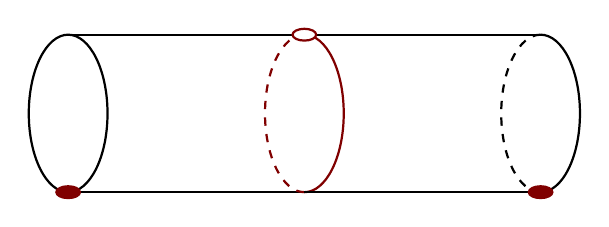
\begin{tikzpicture}
        \begin{scope}
        \draw [thick] (-2,0) arc[start angle=0, end angle=360, x radius=0.5, y radius=1];
        \draw [thick] (-2.5,1) -- (0.5,1);
        \draw [thick] (-2.5,-1) -- (0.5,-1);
        \draw [thick,red!50!black] (0.5,1) arc[start angle=90, end angle=-90, x radius=0.5, y radius=1];
        \draw [thick,red!50!black, dashed] (0.5,-1) arc[start angle=270, end angle=90, x radius=0.5, y radius=1];
        \end{scope}
        \node [ellipse,
    minimum width=3mm,
    minimum height=1.5mm,
    inner sep=0pt,
    fill=red!50!black,
    draw=red!50!black,
    thick] at (-2.5,-1) {};
    \begin{scope}[xshift=3cm]
        \draw [thick] (-2.5,1) -- (0.5,1);
        \draw [thick] (-2.5,-1) -- (0.5,-1);
        \draw [thick] (0.5,1) arc[start angle=90, end angle=-90, x radius=0.5, y radius=1];
        \draw [thick, dashed] (0.5,-1) arc[start angle=270, end angle=90, x radius=0.5, y radius=1];
        \node [ellipse,
    minimum width=3mm,
    minimum height=1.5mm,
    inner sep=0pt,
    fill=red!50!black,
    draw=red!50!black,
    thick] at (0.5,-1) {};
    \end{scope}
    \node [ellipse,
    minimum width=3mm,
    minimum height=1.5mm,
    inner sep=0pt,
    fill=white,
    draw=red!50!black,
    thick] at (0.5,1) {};
    \end{tikzpicture}
    \caption{粘合 $A$ 模型得到 $\mathcal{X} (\phi_1,\phi_2)$。}\label{fig:gluing-A-model-bundle}
\end{figure}

\begin{crl}\label{crl:gluing-mirror-symmetry}
    给定 HMS 对 $(X,Y)$（$X$ 为 Weinstein 扇形、$Y$ 光滑拟射影）与镜像自同构 $(\phi_i,\xi_i)$，$1\leq i\leq k$，则 $A_{\infty}$-范畴之间存在拟等价 \[
        \Perf\mathcal{W}\left[\mathcal{X} (\phi_1,\dotsb ,\phi_k)\right]^{op}\simeq\Coh\mathcal{Y} (\xi_1,\dotsb ,\xi_k)_{dg}
    \]其中 $\mathcal{X} (\phi_1,\dotsb,\phi_k)$ 由粘合 $k$ 个映射柱 $\left(M(X,\phi_i),z_i+z_i^{-1}\right)$ 得到，$\mathcal{Y} (\xi_1,\dotsb ,\xi_k)$ 由粘合 $k$ 个射影丛 $P(Y,\xi_i)$ 得到，粘合规则由图给出\par
    \begin{center}
        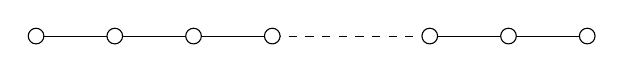
\begin{tikzpicture}
            \draw (0,0) -- (3,0);
            \draw [dashed] (3,0) -- (5,0);
            \draw (5,0) -- (7,0);
            \foreach \x in {0,1,2,3,5,6,7} {
            \node [circle, fill=white, draw=black, inner sep=2pt] at (\x,0) {};
            }
        \end{tikzpicture}
    \end{center}
    图中顶点代表空间 $\left(M(X,\phi_i),z_i+z_i^{-1}\right)$ 与 $P(Y,\xi_i)$，两个顶点之间连一条边，当且仅当它们代表的对象沿纤维/除子粘合。
\end{crl}

\begin{yizhu}[图中的虚线只是「链还没画完」]
实线边表示两块确实沿纤维或除子粘合；虚线边并不表示一种特殊的粘合方式，只表示这条链继续向右延伸、$k$ 可以任意。推论 \ref{crl:gluing-mirror-symmetry-circ} 把首尾两个顶点再连起来之后，链变成环，那条虚线边也就补成了真正的粘合。读这张图时把它当作「粘合示意图」而非几何图形，就不会在虚线上纠缠。
\end{yizhu}

自然，我们还可以把推论 \ref{crl:gluing-mirror-symmetry} 中首尾两个顶点也连起来，从而得到「映射穿孔环面」的镜像对称：

\begin{crl}\label{crl:gluing-mirror-symmetry-circ}
    在与推论 \ref{crl:gluing-mirror-symmetry} 相同的约定下，设 \[
        \mathcal{X}_{\circ} (\phi_1,\dotsb,\phi_k)\quad\text{和}\quad\mathcal{Y}_{\circ} (\xi_1,\dotsb,\xi_k)
    \]分别是按推论 \ref{crl:gluing-mirror-symmetry} 的同一规则、依下图粘合 Weinstein 扇形 $(M(X,\phi_i),z_i+z_i^{-1})$ 与 $\mathbb{P} (\mathcal{O}_Y\oplus\mathcal{L}_{\xi_i})$ 所得的 Weinstein 扇形与代数簇
    \begin{center}
% [原文 p.7]
    \begin{tikzpicture}
        % Circle radius
        \def\R{2}
        % Seven vertices equally spaced around the circle
        \coordinate (v1) at (90:\R);
        \coordinate (v2) at (38.571:\R);
        \coordinate (v3) at (-12.857:\R);
        \coordinate (v4) at (-64.286:\R);
        \coordinate (v5) at (-115.714:\R);
        \coordinate (v6) at (-167.143:\R);
        \coordinate (v7) at (-218.571:\R);
        % Edges, with the fourth-to-fifth edge dashed
        \draw (v1) arc (90:38.571:\R);
        \draw (v2) arc (38.571:-12.857:\R);
        \draw (v3) arc (-12.857:-64.286:\R);
        \draw (v4) arc (-64.286:-115.714:\R);
        \draw[dashed] (v5) arc (-115.714:-167.143:\R);
        \draw (v6) arc (-167.143:-218.571:\R);
        \draw (v7) arc (-218.571:-270:\R);
        % Vertices
        \foreach \vertex in {v1,v2,v3,v4,v5,v6,v7} {
            \node[circle, fill=white, draw=black, inner sep=2pt]
                at (\vertex) {};
        }
    \end{tikzpicture}
\end{center}
    则 $A_{\infty}$-范畴之间存在拟等价 \[
    \Perf\mathcal{W}\left[\mathcal{X}_{\circ} (\phi_1,\dotsb,\phi_k)\right]^{op}\simeq\Coh\mathcal{Y}_{\circ} (\xi_1,\dotsb,\xi_k)_{dg}.
\]
\end{crl}

再配合一些改自 \cite{LK17} 的形变论证，我们应当能实现以椭圆曲线为纤维的纤维丛的镜像对称。

除了把各块粘起来，还可以在 $B$ 侧取线丛的直和，再逐纤维紧化成一个环面丛；相应地，在 $A$ 侧取若干 $T^{\ast}\mathbb{S}^1$ 的乘积，并在底空间上放置相应的停止位，所用规则见 \cite{FLTZ12,Kuwagaki20}。

更精确地说，给定 $A$ 侧的镜像对 $(X;\phi_1,\dotsb ,\phi_k)$ 与 $B$ 侧的镜像对 $(Y;\xi_1,\dotsb, \xi_k)$，其中 $(\phi_1,\dotsb ,\phi_k)$ 是两两交换的辛同胚，再给定整凸多面体 $\Sigma\subseteq\mathbb{R}^k$，可以构造
\[
    \mathcal{X}_{\Sigma} (X;\phi_1,\dotsb ,\phi_k )\coloneqq\left(T^{\ast}\mathbb{T}^n,\Lambda_{\Sigma}\right)\times_{\phi_1,\dotsb ,\phi_n} X\to (T^{\ast}\mathbb{T}^n,\Lambda_{\Sigma})
\]
% [原文 p.8]
作为以 $X$ 为纤维的纤维丛，绕 $\pi_1(\mathbb{T}^n)$ 每个生成元的单值性为 $\phi_i$；同时构造 $\mathcal{Y}_{\Sigma} (Y;\xi_1,\dotsb ,\xi_k)$，它是 $Y$ 上以 $X_{\Sigma}$ 为纤维的纤维丛，$(\xi_1,\dotsb ,\xi_k)$ 刻画其结构主丛。

\begin{yizhu}[原文笔误：$\mathbb{T}^n$ 应为 $\mathbb{T}^k$]
原文这一句前面取的是 $\Sigma\subseteq\mathbb{R}^k$ 与 $\phi_1,\dotsb,\phi_k$，此处却写成 $\mathbb{T}^n$ 与 $\phi_1,\dotsb,\phi_n$；下文又用 $\pi_1(\mathbb{T}^n)$ 的生成元，故按上下文 $n$ 应为 $k$，即环面丛的秩等于多面体 $\Sigma$ 所在空间的维数。译文照原文排印，读到下标 $n$ 时请自行换成 $k$。
\end{yizhu}

\begin{crl}\label{crl:toric-bundle-HMS}
    在与推论 \ref{crl:gluing-mirror-symmetry} 相同的约定下，设 $\Sigma$ 是 $\mathbb{R}^k$ 中的整凸多面体，则 $A_{\infty}$-范畴之间存在拟等价 \[
    \Perf\mathcal{W}\left[\mathcal{X}_{\Sigma} (X;\phi_1,\dotsb ,\phi_k)\right]^{op}\simeq\Coh\left[\mathcal{Y}_{\Sigma} (Y;\xi_1,\dotsb ,\xi_k)\right]_{dg}.
    \]
\end{crl}

\subsection{Hirzebruch 面}

作为另一项应用，我们考察一类特例：作为 $\mathbb{P}^1$ 上 $\mathbb{P}^1$-丛的射影环簇曲面，它们称为 \emph{Hirzebruch 面}。更精确地说，给定非负整数 $n$，Hirzebruch 面 $\mathbb{F}_n$ 是 $\mathbb{P}^1$ 上秩 $2$ 向量丛 $\mathcal{O}\oplus\mathcal{O}_{\mathbb{P}^1} (n)$ 的射影化
\[
    \mathbb{F}_n =\mathbb{P}\left(\mathcal{O}_{\mathbb{P}^1}\oplus\mathcal{O}_{\mathbb{P}^1}(n)\right).
\]
由于 $\mathbb{P}^1$ 是环簇，对一切 $n$，$\mathbb{F}_n$ 都是环簇。

\begin{conceptbox}{Hirzebruch 面}
$\mathbb{F}_n=\mathbb{P}\left(\mathcal{O}_{\mathbb{P}^1}\oplus\mathcal{O}_{\mathbb{P}^1}(n)\right)$ 是 $\mathbb{P}^1$ 上的 $\mathbb{P}^1$-丛；把 $n$ 换成 $-n$ 并交换两个截面即得同构，故同构类型只依赖 $|n|$。$\mathbb{F}_0=\mathbb{P}^1\times\mathbb{P}^1$，而 $\mathbb{F}_1$ 是 $\mathbb{P}^2$ 在一点处的爆破。不同的 $|n|$ 给出互不同构的复结构，但它们作为辛流形可以彼此形变——本文正是借这一点，用同一个映射柱构造在 $\mathbb{F}_n$ 上造出一族「异域」的 Weinstein 扇形（推论 \ref{crl:exotic-Weinstein-structure}）。
\par\smallskip\noindent{\footnotesize 参考：Hartshorne, \emph{Algebraic Geometry}, V.2；本文 §1c。}
\end{conceptbox}

注意，尽管对一切环簇都已知道凝聚—可构造对应，当环簇不是 Fano 时，该结果与 Hori--Vafa \cite{HV00} 的镜像构造并不相容。例如，Hori--Vafa 超势 $W_n$ 的临界点个数不等于镜像 $\mathbb{F}_n$ 的量子上同调秩 \cite[Example 8.2]{FOOO10}。SYZ 镜像构造——如 Auroux \cite{Auroux09} 所解释、后由 Jing \cite{Jing26} 所研究——则高度非平凡，可能涉及把无穷多块图卡粘在一起。

借助定理 \ref{thm:HMS-projective-bundle}，我们给出 $\mathbb{F}_n$ 的同调镜像的一个相当直接的描述。

\begin{crl}\label{crl:mirror-to-Hirzebruch}
    记 \[
        \rF_n =\left(M((\mathbb{C}^{\ast}, x+1/x),\phi^n),z+1/z\right)
    \]为一个 Landau--Ginzburg 模型，其中 $\phi\colon\mathbb{C}^{\ast}=T^{\ast}\mathbb{S}^1\to T^{\ast}\mathbb{S}^1$ 是沿零截面的 Dehn 扭转。则作为带边流形有微分同胚，作为带超势的全纯流形有同构 \[
        \rF_n\cong\left(\mathbb{C}^{\ast}\times\mathbb{C}^{\ast}, x+1/x+y+1/y\right)
    \]并且 $A_{\infty}$-范畴之间存在拟等价 \[
        \Perf\mathcal{W} (\rF_n)^{op}\simeq\Coh\left(\mathbb{F}_n\right)_{dg}.
    \]
\end{crl}

\begin{yizhu}[$\rF_n$ 的记号与「微分同胚不算辛同构」]
$\rF_n$ 中的花体 F 是翻转的 $\mathrm{F}$——它表示 $\mathbb{F}_n$ 的镜像，不是一个新曲面。推论 \ref{crl:mirror-to-Hirzebruch} 同时给出两个层面的结论：作为带边流形微分同胚，作为带超势的全纯流形同构。但微分同胚远弱于精确辛同胚：前者只比对光滑结构，后者要求 Liouville 形式本身被拉回；这里两个结论并不蕴含 $\rF_n$ 与 $\left(\mathbb{C}^{\ast}\right)^2$ 在辛意义下相同，下一推论的「异域」正由此而来。
\end{yizhu}

特别地，由 Bondal--Orlov \cite{BO01} 与 Bridgeland--Maciocia \cite{BM01} 的工作可知，$\Coh (\mathbb{F}_n)\cong\Coh (\mathbb{F}_m)$ 当且仅当 $m=n$，于是立即得到下面这个或许有趣的推论：

\begin{crl}\label{crl:exotic-Weinstein-structure}
    $\rF_n$ 与 $\rF_m$ 精确辛同胚，当且仅当 $m=n$。
\end{crl}

因此，尽管所有 $\rF_n$ 作为 Landau--Ginzburg 对都彼此微分同胚且同构，它们之间却并非精确辛同胚；于是它们构成一族「异域」的 Weinstein 扇形，因为精确辛同胚保持 Fukaya 范畴 \cite{HS26}。不过应当注意，Fukaya 范畴无法区分它们的凸完成，因此我们并不知道这是否在 $\left(\mathbb{C}^{\ast}\right)^2$ 上造出了异域的 Weinstein 结构。另一个疑问是局部同调镜像与 Hori--Vafa 构造之间的关系，即

\begin{conceptbox}{异域 Weinstein 结构}
同一个光滑流形上可以承载无穷多个两两不精确辛同构的 Weinstein 结构：它们作为辛流形彼此不同，其上的包裹 Fukaya 范畴却可能等价。本文由 Hirzebruch 面 $\mathbb{F}_n$（$n\ge 0$）造出这样一族结构——$\rF_n$ 作为带边流形、作为带超势全纯流形都同构，精确辛同构类却随 $n$ 变化，故称「异域」。它说明 A 模型经 $\Coh$ 的等价能看见 B 侧的部分复结构差异，却看不见凸完成层面的差异，这对「Weinstein 结构的辛同胚分类」与「Fukaya 范畴的分类」之间的落差给出了一个具体刻度。
\par\smallskip\noindent{\footnotesize 参考：Kartal, arXiv:2204.04928；本文 §1c 推论 \ref{crl:exotic-Weinstein-structure}。}
\end{conceptbox}

\begin{ques}\label{Q:HV-vs-LHMS}
    局部同调镜像 $\rF_n$ 与 Hori--Vafa 镜像 $\left((\mathbb{C}^{\ast})^2,W_n\right)$ 之间是什么关系？
\end{ques}

回答这个问题有望通过族 Floer 纲领，得到 Hirzebruch 面所期望的 SYZ 镜像。

\begin{keytakeaways}
  \item 多重单值性的机制：把 $k$ 个射影丛 $P(Y,\xi_i)$ 沿零截面与无穷远截面粘成节点链，B 侧的 $\Coh$ 由真下降（同伦前推）拼出；A 侧对应把 $k$ 个映射柱 $(M(X,\phi_i),z_i+z_i^{-1})$ 沿停止位粘成 Weinstein 扇形。推论 \ref{crl:gluing-mirror-symmetry} 与 \ref{crl:gluing-mirror-symmetry-circ} 分别是开链与闭环两种粘法，而推论 \ref{crl:toric-bundle-HMS} 把同一套下降换成环面丛。
  \item 链式粘合的单值性对应很强：B 侧的 $\{P(Y,\xi_i)\}$ 沿截面粘、A 侧的 $\{z_i\}$ 坐标在 $0$ 与 $\infty$ 处相接，$0/\infty$ 的对应关系是全部计算的账本，稍一错位就会得到不同的扇形。
  \item Hirzebruch 面给出显式例子：$\rF_n$ 作为带超势全纯流形，同构于 $\mathbb{C}^{\ast}_x\times\mathbb{C}^{\ast}_y$ 上带超势 $x+1/x+y+1/y$ 的模型，但 $n$ 不同则精确辛同构类不同，根源是 B 侧的 $\Coh (\mathbb{F}_n)$ 不同（推论 \ref{crl:exotic-Weinstein-structure}）。
\end{keytakeaways}

\subsection{全文结构}

在第 \ref{sec:proof-of-theorems} 节中，我们给出主定理各条陈述的全部证明，技术细节留到后面的各节。在第 \ref{sec:algebraic-preparations} 节中，我们给出全文要用到的高阶代数及其相应运算的基本定义。第 \ref{sec:Fukaya-category-discrete-quotient} 节致力于 $A$ 侧计算所需的若干新的结构性结果，第 \ref{sec:G-equiv-sheaves} 节与第 \ref{sec:kunneth-formula} 节则为 $B$ 侧计算准备必要的材料。更具体地说，第 \ref{sec:G-equiv-sheaves} 节给出 $G$-等变层范畴的基本性质，第 \ref{sec:kunneth-formula} 节建立关键公式：等变层的 K\"unneth 公式。在附录 \ref{sec:Eilenberg-Zilber-constraction} 中，我们回顾经典的 Eilenberg--Zilber 构造，并把它改造到本文的情形，它将用于 Künneth 公式 \ref{thm:Kunneth-embedding} 的证明。

% [原文 p.9]
\subsection*{致谢}

本文的主要想法源于 2025 年末作者在波恩马克斯·普朗克数学研究所逗留期间与 Tim Hu、Maximilian Schimpf 的讨论，我们感谢与他们的所有有益讨论。

我们还要感谢 Yanki Lekili、Cheuk Yu Mak、Longke Tang 与 Bingyu Zhang 的许多有益讨论与建议。

S.-Y. Liu 由德国研究基金会（Deutsche Forschungsgemeinschaft，DFG）在德国卓越战略（Germany's Excellence Strategy）项目 GZ 2047/1、Projekt-ID 390685813 下资助。

Kyungmin Rho 感谢波恩马克斯·普朗克数学研究所的款待与资助。

\subsection*{AI 使用声明}

当作者试图证明不同构的 Hirzebruch 面上的凝聚层复形不拟同构时，文献 \cite{BM01} 的结果是在大语言模型（LLM）的帮助下找到的。作者当时认为应当存在比 \cite{BM01} 这一过强结果更合适的参考文献，而 LLM 坚称该结果不可或缺。

作者用 LLM 探究 \ref{defn:wrapped-Fukaya-cat-inf-sectors} 中「小」Fukaya 范畴的定义是否就是 $\mathcal{W}^{big} (X)$ 中紧对象的范畴，未能成功。在与 Bingyu Zhang、Longke Tang 讨论之后，作者确信需要一些必要的几何论证，于是决定把这一点留作后续问题。

把 $A_{\infty}$-范畴 $\mathcal{A}$ 关于群 $G$ 的同伦商与 $A_{\infty}$-轨道范畴联系起来的文献 \cite{Christ26}，同样是在 LLM 的帮助下找到的。

在推论 \ref{crl:gluing-mirror-symmetry} 的证明中，作者请 LLM 把第一个巨大的公式拆成两行：原始代码输入 LLM，输出经检查后直接复制进文件。

作者曾尝试为命题 \ref{prp:dg-enhancement} 的证明寻找更多参考文献，LLM 未能给出超出作者已有知识范围的答案。

作者用 LLM 把 Seidel \cite{Seidel08} 的右模作用改写为左模作用，检查后把生成的代码复制进文件。

% ch02 译文：原文 §2 定理的证明（main.tex 第 365--515 行）
\section{定理的证明\label{sec:proof-of-theorems}}

本节给出引言中各条结论的证明，技术细节留待后面的各节。

\subsection{预备与蓝图}

全文在 $A$ 模型一侧把所有辛流形 $X$ 都视作 \emph{Liouville 扇形}，其定义见定义 \ref{defn:Liouville-sector-inf}。对有限型的 Liouville 扇形，其包裹 Fukaya 范畴已在 \cite{GPS20} 中定义，并具有 \cite{GPS24S} 所解释的许多良好函子性质。

给定 Liouville 扇形 $X$ 的精确辛同胚 $\phi\colon X\to X$，可以定义\emph{映射柱}
\[
    M (X,\phi )\coloneqq X\times_{\phi}\mathbb{C}^{\ast}\coloneqq\frac{T^{\ast}\mathbb{R}\times X}{(z,x)\sim (z+1,\phi (x))}
\]
% [原文 p.10]
它可以看作乘积空间 $X\times\mathbb{C}$ 在 $\mathbb{Z}$-作用下的商，该作用在 $X$ 上按 $\phi$ 作用、在 $\mathbb{C}$ 上按平移 $1$ 作用。

\begin{yizhu}[Kartal 的修改在改什么]
公式里写的是 $T^{\ast}\mathbb{R}\times X$，正文却说乘积 $X\times\mathbb{C}$：因为 $T^{\ast}\mathbb{R}\cong\mathbb{R}^2\cong\mathbb{C}$，坐标 $z$ 就是复坐标，两者是同一空间。光滑层面取商没有问题，但乘积 Weinstein 结构一般并不 $\mathbb{Z}$-不变，直接取商会丢掉 Liouville 形式、破坏凸性；Kartal 的修改正是把辛结构调整成 $\mathbb{Z}$-不变而仍为 Weinstein，命题 \ref{prp:Fukaya-cat-mapping-cylinder} 中「在范畴层面取商」的写法才说得通。
\end{yizhu}

其 Weinstein 结构按定义 \ref{defn:G-invariant-Weinstein-sector} 由 $X\times\mathbb{C}$ 诱导；更具体地说，是借助 Kartal \cite{Kartal21} 的想法对乘积 Weinstein 结构作一次修改而得到，该修改在命题 \ref{prp:Kartal-modification-Weinstein} 中完成。带停止位的 $T^{\ast}\mathbb{R}$ 的包裹 Fukaya 范畴（停止位取 $e^z+e^{-z}$ 在无穷远处的原像）已在例 \ref{exmp:mirror-to-Coh-G-P1} 中算出，于是有

\begin{prp}\label{prp:Fukaya-cat-mapping-cylinder}
    $\mathcal{W} (M(X,\phi),z+1/z)\simeq\left(\mathcal{W} (T^{\ast}\mathbb{R}, e^z+e^{-z})\otimes\mathcal{W} (X)\right)/\mathbb{Z}$.
\end{prp}
\begin{proof}
    由 Künneth 公式 \ref{crl:Kunneth-Fukaya-infinite} 并结合 \cite{Ornaghi25} 中 $A_{\infty}$-范畴张量积的定义，我们得到 $A_{\infty}$-范畴的拟等价 \[
        \mathcal{W} (T^{\ast}\mathbb{R},e^z+e^{-z})\otimes\mathcal{W} (X)\hookrightarrow\mathcal{W} (T^{\ast}\mathbb{R}\times X, e^z+e^{-z}).
    \]由定理 \ref{thm:wrapped-Fukaya-quotient}，由于我们已把 $T^{\ast}\mathbb{R}\times X$ 上的 Weinstein 结构改成 $\mathbb{Z}$-不变的，便知 \[
        \mathcal{W} (M(X,\phi),z+z^{-1})=\mathcal{W}\left((T^{\ast}\mathbb{R}\times X,e^z+e^{-z})/\mathbb{Z}\right)\simeq\mathcal{W} (T^{\ast}\mathbb{R}\times X,e^z+e^{-z})/\mathbb{Z}
    \]命题得证。
\end{proof}

在镜像一侧，我们从代数簇 $Y$ 以及特征类 $\xi\in CH^2 (Y)$ 的选取出发，后者定义 $Y$ 上的全纯线丛 $L_{\xi, Y}$。去掉零截面 $Y\hookrightarrow L_{\xi, Y}$ 所得的子丛 $L_{\xi,Y}^{\times}$ 因而是 $Y$ 上的主 $\mathbb{G}_m$-丛，从而带有自由的代数 $\mathbb{G}_m$-作用。于是有

\begin{thm}\label{thm:twisted-tensor-P1-bundle}
    设 $Y$ 光滑且拟射影，则存在 dg 范畴的拟等价\footnote{此处的 $\Perf$ 定义与通常定义不同，见定义 \ref{dfn:dg-enhancement-Coh}。}
\[
\Perf_{\mathbb{G}_m}(\mathbb{P}^1)_{\dg}
\underset{((1),\mathcal{L}(\xi)\otimes-)}{\otimes}
\Perf(Y)_{\dg}
\rightarrow
\Perf(P(Y,\xi))_{\dg}.
\]
\end{thm}

\begin{conceptbox}{扭 Künneth 公式}
普通的 Künneth 公式把两个空间的同调的张量积与乘积空间的同调联系起来；在范畴层面，它呈现为 $\Perf (X)\otimes\Perf (Y)\simeq\Perf (X\times Y)$ 型的等价。扭 Künneth 公式处理的是「张量积带一个由线丛或群作用给出的扭」的情形：此时普通张量积要换成带扭的版本，常见的做法是只取某个权重、某个特征的部分。本文两次用到它：定理 \ref{thm:twisted-tensor-P1-bundle} 中的扭由线丛 $\mathcal{L} (\xi)$ 给出，§6 中则用它把 $\mathbb{G}_m$-等变层与 Fukaya 范畴的 Künneth 对接起来。忽略扭、按普通张量积理解，得到的函子会漏掉权重指标，半正交分解也拼不起来。
\par\smallskip\noindent{\footnotesize 参考：nLab, Künneth theorem（ncatlab.org/nlab/show/Künneth+theorem）；本文 §2a、§6c。}
\end{conceptbox}

\begin{yizhu}[脚注里的 $\Perf$ 不是平常的 $\Perf$]
定理 \ref{thm:twisted-tensor-P1-bundle} 中的 $\Perf_{\mathbb{G}_m}(\mathbb{P}^1)_{\dg}$ 并非通常的 $\Perf(\mathbb{P}^1)$：下标表示取 $\mathbb{G}_m$-等变的完美模，其定义见定义 \ref{dfn:dg-enhancement-Coh}。这个差别至关重要——只有等变版本才与 $\Perf\mathcal{W}(T^{\ast}\mathbb{R},e^z+e^{-z})$ 拟等价；若按非等变版本理解，下面的扭 Künneth 公式与 $\mathbb{Z}$-轨道范畴都接不上。
\end{yizhu}

\begin{proof}
    注意 \[
        Y=\left[\frac{L(Y,\xi)^{\times}}{\mathbb{G}_m}\right],
    \]因此有拟等价 $\Perf (Y)_{dg}\simeq\Perf_{\mathbb{G}_m} (L(Y,\xi)^{\times})_{dg}$。注意 $\Perf_{\mathbb{G}_m} (\mathbb{P}^1)_{dg}\otimes\Perf_{\mathbb{G}_m} (L(Y,\xi)^{\times})_{dg}$ 上的作用 $((1),\mathcal{L} (\xi)\otimes -)$ 是对角的，由扭 K\"unneth 公式得到拟嵌入 \[
        \Perf_{\mathbb{G}_m} (\mathbb{P}^1)\otimes_{\mathbb{Z}=\widehat{\mathbb{G}}_m}\Perf_{\mathbb{G}_m} (L(Y,\xi)^{\times})_{dg}\hookrightarrow\Perf_{\mathbb{G}_m} (\mathbb{P}^1\times L(Y,\xi)^{\times} )_{dg}\cong\Perf (P(Y,\xi))_{dg},
    \]于是只需证明该拟嵌入本质满射。Orlov \cite{Orlov92} 的工作表明，在此情形存在三角范畴的半正交分解 \[
    D\Perf (P(Y,\xi))_{dg}\simeq\langle D\Perf(Y)_{-1}, D\Perf(Y)_0\rangle,
% [原文 p.11]
    \]它表明形如 $\pi^{\ast}\mathcal{F}$ 与 $\pi^{\ast}\mathcal{F}\otimes\mathcal{O}_{P(Y,\xi)} (1)$ 的对象生成 $\Perf(P(Y,\xi))_{dg}$，其中 $\mathcal{O}_{P(Y,\xi)} (1)$ 是限制到每根纤维为 $\mathcal{O}_{\mathbb{P}^1} (1)$ 的可逆层，$\mathcal{F}\in\Perf (Y)$。注意这些对象是$\Perf_{\mathbb{G}_m} (\mathbb{P}^1)_{dg}\widetilde{\otimes}\Perf (Y)_{dg}$ 中对象 $\mathcal{O}_{\mathbb{P}^1} (i)\widetilde{\otimes}\mathcal{F}$ 的像，因此该拟嵌入的像生成目标 dg 范畴。
\end{proof}

由 \cite{FLTZ12} 与例 \ref{exmp:mirror-to-Coh-G-P1} 显然有 $\Perf_{\mathbb{G}_m} (\mathbb{P}^1)_{dg}\simeq\Perf\mathcal{W} (T^{\ast}\mathbb{R},e^z+e^{-z})$，至此材料已经备齐，可以完成证明。

\begin{proof}[定理 \ref{thm:HMS-projective-bundle} 的证明]
    由假设 $\Perf\mathcal{W} (X)^{op}\simeq\Coh (Y)_{dg}=\Perf (Y)_{dg}$，又由前述讨论 $\Perf\mathcal{W} (T^{\ast}\mathbb{R},e^z+e^{-z})^{op}\simeq\Perf_{\mathbb{G}_m} (\mathbb{P}^1)_{dg}$，故它们的张量积之间有拟等价 \[
        \Perf\mathcal{W} (T^{\ast}\mathbb{R},e^z+e^{-z})^{op}\otimes\Perf\mathcal{W} (X)^{op}\simeq\Perf_{\mathbb{G}_m} (\mathbb{P}^1)_{dg}\otimes\Perf (Y)_{dg}.
    \]在 $A$ 模型一侧，乘积空间上的 $\mathbb{Z}$-作用由 $T^{\ast}\mathbb{R}$ 上的平移 $1$ 与 $\mathcal{W} (X)$ 上的辛同胚 $\phi$ 给出，它与 $B$ 侧来自 $\mathbb{G}_m$-作用的范畴 $\mathbb{Z}$-作用相合。于是取 $\mathbb{Z}$-轨道范畴，再结合命题 \ref{prp:Fukaya-cat-mapping-cylinder} 与定理 \ref{thm:twisted-tensor-P1-bundle}，即完成证明。
\end{proof}

\begin{conceptbox}{映射柱与停止位}
映射柱 $M(X,\phi)$ 是把 $T^{\ast}\mathbb{R}\times X$ 沿 $\mathbb{Z}$-作用 $(z,x)\sim(z+1,\phi (x))$ 取商得到的空间，它把自同胚 $\phi$ 的「单值性」实现成一个空间：沿 $z$ 方向绕一圈，纤维上的点就按 $\phi$ 搬一次。最简单的例子是 $\phi$ 取 $T^{\ast}\mathbb{S}^1=T^{\ast}\mathbb{R}/\mathbb{Z}$ 上的平移，此时映射柱退化为映射环面，$\phi$ 即 Dehn 扭转；本文推论 \ref{crl:mirror-to-Hirzebruch} 正是把这个例子与 $\Coh (\mathbb{F}_n)$ 对上。要谈包裹 Fukaya 范畴，还得在扇形边界上指定停止位：Reeb 流只允许在停止位处终结，于是「哪些无穷远处的 Reeb 轨道被算进来」就成了可设计的参数，$\mathcal{W}$ 也因此依赖停止位。本文的映射柱把停止位取成 $e^z+e^{-z}$ 在无穷远处的原像。
\par\smallskip\noindent{\footnotesize 参考：Kartal, arXiv:2204.04928；Sylvan, arXiv:1601.05080；本文 §2a、§2d。}
\end{conceptbox}

\begin{proof}[推论 \ref{crl:mirror-symmetry-line-principal-bundles} 的证明]
    只需证明包含函子 $i_0\colon\Coh (Y)\to\Coh (P(Y,\xi))$ 与 Orlov 函子 $\cup_0\colon\mathcal{W} (X)\to\mathcal{W} (M(X,\phi),z+z^{-1})$ 互为镜像。注意由构造，$i_0$ 可分解为 \[
        \Perf (Y)_{dg}\xrightarrow{i_0}\Perf (Y)_{dg}\otimes\Perf_{\mathbb{G}_m}(\mathbb{P}^1)_{dg}\to\Perf (P(Y,\xi))_{dg},
    \]类似地 $\cup_0$ 可分解为 \[
        \Perf\mathcal{W} (X)^{op}\xrightarrow{\cup_0}\Perf\mathcal{W} (X\times (T^{\ast}\mathbb{R},e^z+e^{-z}))^{op}\to\Perf\mathcal{W} (M(X,\phi),z+z^{-1})^{op},
    \]其中第二个映射都是对 $\mathbb{Z}$-作用取商，而我们已经知道二者互为镜像。在 $B$ 侧，函子 $i_0$ 把任意 $\mathcal{F}\in\Coh (Y)$ 送到层 $\mathcal{F}\otimes\mathcal{O}_0 [0]$；在 $A$ 侧，$\cup_0$ 把 $L\in\mathcal{W} (X)$ 送到 $L\otimes D[0]$，其中 $D[0]\in\Perf\mathcal{W} (T^{\ast}\mathbb{R},e^z+e^{-z})^{op}\simeq\Perf_{\mathbb{G}_m} (\mathbb{P}^1)_{dg}$ 是以标号为 $0$ 的停止位为边界的链接圆盘，在相差一个平移的意义下等同于 $\mathcal{O}_0 [0]$。因此 $i_0$ 与 $\cup_0$ 互为镜像，再取局部化即完成证明。主丛情形的证明基本相同，只需把 $0$ 换成 $\infty$。
\end{proof}

\begin{yizhu}[{链接圆盘 ${D[0]}$ 与 $0/\infty$ 的不对称}]
$D[0]$ 是一块以标号 $0$ 的停止位为边界的链接圆盘，它在 $\Perf\mathcal{W}(T^{\ast}\mathbb{R},e^z+e^{-z})^{op}$ 中对应 $\mathbb{P}^1$ 在零截面处的结构层 $\mathcal{O}_0$（差一个平移）。这里的 $op$ 不是装饰：取 $op$ 之后，「圆盘对应点」才成为函子层面的对应，$\cup_0$ 的方向也才与 $i_0$ 一致。主丛情形把 $0$ 换成 $\infty$、把 $\mathcal{O}_0$ 换成 $\mathcal{O}_\infty$ 即可，但两条推论的停止位选择不能混用，否则拿到的是另一对函子。
\end{yizhu}

\subsection{扇形下降与真下降}

接下来处理推论 \ref{crl:gluing-mirror-symmetry} 与推论 \ref{crl:gluing-mirror-symmetry-circ} 的证明。尽管陈述相当一般，我们只需理解 $k=2$ 的情形；而这可由例 \ref{exmp:wrapped-Fukaya-cat-twice-punctured-equivariant} 的讨论得到。

给定 $B$ 模型数据 $(Y,\xi_1,\xi_2)$，我们把两个射影丛沿 $0$ 处截面与 $\infty$ 处截面粘起来，构造空间
\[
    \mathcal{Y} (\xi_1,\xi_2)=P(Y,\xi_1)\cup_Y P(Y,\xi_2)
\]
注意 $\mathcal{Y} (\xi_1,\xi_2)$ 上有 $\mathbb{G}_m^2$-作用：它由每个 $P(Y,\xi_i)$ 上的 $\mathbb{G}_m$-作用给出，而这些作用在另一个分支上平凡地延拓。由真前推图表
\[
    \begin{tikzcd}
        Y\arrow[r,"i_0"]\arrow[d,"i_{\infty}"]&P(Y,\xi_2)\arrow[d]\\ 
        P(Y,\xi_1)\arrow[r]&\mathcal{Y} (\xi_1,\xi_2)
    \end{tikzcd}
\]
直接得到商叠的真前推图表\footnote{这直接由商叠的定义与赋值判据得到，参见例如 \cite{Alper26}。} \[
    \begin{tikzcd}
        {[Y/\mathbb{G}_m^2]}\arrow[r,"i_0"]\arrow[d,"i_{\infty}"]&{\big[P(Y,\xi_2)/\mathbb{G}_m^2\big]}\arrow[d]\\ 
        \big[P(Y,\xi_1)/\mathbb{G}_m^2\big]\arrow[r]&\big[\mathcal{Y}(\xi_1,\xi_2)/\mathbb{G}_m^2\big]
    \end{tikzcd}
\]
% [原文 p.12]
对闭浸入的前推图表，拟凝聚层的前推公式（它由 Gaitsgory--Rozenblyum \cite[Theorem A.1.2]{GR17II} 连同拟凝聚层的下降性质得到）给出同伦前推图表 \[
    \begin{tikzcd}
        {\IndCoh [Y/\mathbb{G}_m^2]_{\infty}}\arrow[r,"i_0"]\arrow[d,"i_{\infty}"]&{\IndCoh\big[P(Y,\xi_2)/\mathbb{G}_m^2\big]_{\infty}}\arrow[d]\\ 
        \IndCoh\big[P(Y,\xi_1)/\mathbb{G}_m^2\big]_{\infty}\arrow[r]&\IndCoh\big[\mathcal{Y}(\xi_1,\xi_2)/\mathbb{G}_m^2\big]_{\infty}
    \end{tikzcd}
\]又因为闭浸入把凝聚层前推为凝聚层，凝聚层的同一图表也是同伦前推图表。利用 \cite{Cohn16} 证明的 $dg$-范畴与 $\infty$-范畴之间的拟等价，我们有

\begin{prp}\label{prp:pushforward-coherent-stack}
    存在 $A_{\infty}$-范畴的拟等价 \[
        \Coh_{\mathbb{G}_m^2}\mathcal{Y} (\xi_1,\xi_2)_{dg}\simeq\hocolim\left(\Perf_{\mathbb{G}_m^2} (P(Y,\xi_1))_{dg}\leftarrow\Perf_{\mathbb{G}_m^2} (Y)_{dg}\rightarrow\Perf_{\mathbb{G}_m^2} (P(Y,\xi_2))_{dg}\right).
    \]
\end{prp}

现在转向镜像一侧。由于额外的 $\mathbb{G}_m$-作用在 $Y$ 上也是平凡的，我们有 $[P(Y,\xi_i)/\mathbb{G}_m^2]=[\mathbb{P}^1/\mathbb{G}_m]\times Y\times [\mathrm{pt}/\mathbb{G}_m]$。由于 $\Perf_{\mathbb{G}_m} (\mathbb{P}^1)_{dg}\simeq\Perf\mathcal{W} (T^{\ast}\mathbb{R},e^z+e^{-z})$，只需理解 $[\mathrm{pt}/\mathbb{G}_m]$ 的同调镜像对称。

\begin{yizhu}[两个 $\mathbb{G}_m$ 各管一个方向]
$\mathcal{Y}(\xi_1,\xi_2)$ 上的 $\mathbb{G}_m^2$ 中，一个 $\mathbb{G}_m$ 作用在 $\mathbb{P}^1$ 纤维方向（它来自射影丛的等变结构），另一个沿 $L(Y,\xi_i)^{\times}\to Y$ 的主丛方向作用（把 $Y$ 展成 $L^{\times}/\mathbb{G}_m$ 的那个作用）。两者交换，故有分解 $[P(Y,\xi_i)/\mathbb{G}_m^2]=[\mathbb{P}^1/\mathbb{G}_m]\times Y\times[\mathrm{pt}/\mathbb{G}_m]$。把哪个因子当作「纤维方向」、哪个当作「底」，决定了下一步该对谁用层—Floer 对应，这是 §2b 全部计算的账本。
\end{yizhu}

\begin{lmm}
    存在 $A_{\infty}$-范畴的拟等价 \[
        \Perf\mathcal{W}\left(\bigsqcup_{i\in\mathbb{Z}}T^{\ast}[0,1]\right)^{op}\simeq\Perf_{\mathbb{G}_m} (\mathrm{pt})_{dg}.
    \]
\end{lmm}
\begin{proof}
    注意左端是同伦余积 \[
       \Perf \mathcal{W}\left(\bigsqcup_{i\in\mathbb{Z}}T^{\ast} [0,1]\right)^{op}\simeq\coprod_{i\in\mathbb{Z}}\Perf\mathcal{W} (T^{\ast} [0,1])^{op}\simeq \coprod_{i\in\mathbb{Z}}\Perf (\mathrm{pt})_{dg}\simeq\coprod_{i\in\mathbb{Z}}\Perf\field\text{-}\Mod_{dg},
    \]另一方面，由 \cite[Proposition 4.9]{TV18} 知 $\mathbb{G}_m$-等变拟凝聚范畴 $\QCoh_{\mathbb{G}_m} (\mathrm{pt})_{dg}\simeq\Rep_{\Bbbk} (\mathbb{G}_m)_{dg}$ 等价于 $\mathbb{G}_m$ 的表示范畴；又因线性 $\mathbb{G}_m$-表示无非是 $\mathbb{Z}$-分次，$\Rep_{\Bbbk} (\mathbb{G}_m)_{dg}$ 等价于带一个额外 $\mathbb{Z}$-分次的 $\field$-向量空间复形范畴。取紧对象，并利用 $\Perf_{\mathbb{G}_m} (\mathrm{pt})_{dg}$ 是 $\QCoh_{\mathbb{G}_m} (\mathrm{pt})_{dg}$ 的紧子范畴 \cite{BZFN10} 这一事实，便知 \[
        \Perf_{\mathbb{G}_m} (\mathrm{pt})_{\infty}\simeq\left(\Rep_{\Bbbk} (\mathbb{G}_m)_{\infty}\right)^{\omega}\simeq\coprod_{i\in\mathbb{Z}}\Perf\Bbbk\text{-}\Mod_{\infty}
    \]最后用 \cite{Cohn16} 中 $dg$-范畴与 $\Bbbk$-线性稳定 $\infty$-范畴的等价完成证明。
\end{proof}

% [原文 p.13]
由该引理与前述讨论，得到 $A_{\infty}$-范畴的拟等价 \begin{align}\label{eq:equivariant-mirror-Gm2}
    \begin{split}
    \Perf\mathcal{W}\left(\bigsqcup_{i\in\mathbb{Z}} (T^{\ast}\mathbb{R},e^z+e^{-z})\right)^{op}&\simeq\Perf\mathcal{W} (T^{\ast}\mathbb{R},e^z+e^{-z})^{op}\otimes\Perf_{\mathbb{G}_m} (\mathrm{pt})\\ 
    &\simeq\Perf_{\mathbb{G}_m} (\mathbb{P}^1)\otimes\Perf_{\mathbb{G}_m} (\mathrm{pt})\simeq\Perf_{\mathbb{G}_m^2} (\mathbb{P}^1).
    \end{split}
\end{align}
\begin{proof}[推论 \ref{crl:gluing-mirror-symmetry} 的证明]
    如前所述，只需对选定的镜像数据 $(X,\phi_1,\phi_2)$ 与 $(Y,\xi_1,\xi_2)$ 验证 \[
        \Perf\mathcal{W}\left(\mathcal{X} (\phi_1,\phi_2)\right)^{op}\simeq\Coh\left(\mathcal{Y}(\xi_1,\xi_2)\right)
    \]等价 \eqref{eq:equivariant-mirror-Gm2} 连同对镜像函子的分析，给出下述两个图表之间的拟等价 \[
\begin{aligned}
&\Perf\left(
\begin{tikzcd}
\mathcal{W}\left(\bigsqcup_{\mathbb{Z}^2}T^{\ast}[0,1]\right)
  \arrow[r]\arrow[d]
&
\mathcal{W}\left(\bigsqcup_{\mathbb{Z}}(\mathbb{C},e^{z_1}+e^{-z_1})\right)
\\
\mathcal{W}\left(\bigsqcup_{\mathbb{Z}}(\mathbb{C},e^{z_2}+e^{-z_2})\right)
&
\end{tikzcd}
\right)^{op}
\\[1em]
&\simeq
\left(
\begin{tikzcd}
\Coh[\mathrm{pt}/\mathbb{G}_m^2]_{dg}\arrow[r]\arrow[d]
&
\Coh[\mathbb{P}^1/\mathbb{G}_m^2]_{dg}
\\
\Coh[\mathbb{P}^1/\mathbb{G}_m^2]_{dg}
&
\end{tikzcd}
\right).
\end{aligned}
\]因此 $\Perf\mathcal{W} (\mathcal{X})^{op}\simeq\Coh_{\mathbb{G}_m^2} (\mathbb{P}^1\cup_{0\sim\infty}\mathbb{P}^1)$，再张量上 $\Perf\mathcal{W} (X)^{op}\simeq\Coh (Y)_{dg}$ 并对典范 $\mathbb{Z}^2$-作用取商，即得所需的范畴等价。
\end{proof}
\begin{proof}[推论 \ref{crl:gluing-mirror-symmetry-circ} 的证明]
    与推论 \ref{crl:gluing-mirror-symmetry} 的证明完全平行。
\end{proof}

\subsection{环面丛}

注意，由等变凝聚—可构造对应 \cite{FLTZ11}，有 dg 范畴的拟等价 \[
    \Sh_{\widetilde{\Lambda}_{\Sigma}} (\mathbb{R}^n)^{cc}\simeq\Coh_{\mathbb{G}_m^n} (X_{\Sigma})
\]只要 $X_{\Sigma}$ 是光滑环簇。这里 $\Sh_{\widetilde{\Lambda}_{\Sigma}} (\mathbb{R}^n)^{cc}$ 是紧支集可构造层复形的 dg 范畴，而由 \cite[Lemma 4.18]{GPS24M} 有 \[
    \Sh_{\widetilde{\Lambda}_{\Sigma}} (\mathbb{R}^n)^{cc}\simeq\Sh_{\widetilde{\Lambda}_{\Sigma}} (\mathbb{R}^n)^{\omega},
\]由层—Floer 对应 \ref{prp:inf-type-sheaf-Floer-Rn} 知它拟等价于包裹 Fukaya 范畴 $\Perf\mathcal{W} (T^{\ast}\mathbb{R}^n,\widetilde{\Lambda}_{\Sigma})^{op}$。于是只要 $X_{\Sigma}$ 光滑（等价地，$\Sigma$ 是整凸多面体），就有 $A_{\infty}$-范畴的拟等价 \[
    \Perf\mathcal{W} (T^{\ast}\mathbb{R}^n,\widetilde{\Lambda}_{\Sigma})^{op}\simeq\Coh_{\mathbb{G}_m^n} (X_{\Sigma})
\]
\begin{proof}[推论 \ref{crl:toric-bundle-HMS} 的证明]
    在 $A$ 侧有 \[
        \mathcal{W}\left[\mathcal{X}_{\Sigma} (X;\phi_1,\dotsb ,\phi_k)\right]\simeq\mathcal{W} (T^{\ast}\mathbb{R}^k,\widetilde{\Lambda}_{\Sigma})\otimes_{\mathbb{Z}^k}\mathcal{W} (X),
    \]而在 $B$ 侧可以写 $\mathcal{Y}_{\Sigma} (Y;\xi_1,\dotsb ,\xi_k)=\left(X_{\Sigma}\times \prod_{i=1}^k L(Y,\xi_i)^{\times}\right)/\mathbb{G}_m^k$，于是 \[
        \Coh\left[\mathcal{Y} (Y;\xi_1,\dotsb ,\xi_k)\right]\simeq\left[\Coh_{\mathbb{G}_m^k} (X_{\Sigma})\otimes\Coh_{\mathbb{G}_m^k} \left(\prod_{i=1}^kL(Y,\xi_i)^{\times}\right)\right]\Big/\mathbb{G}_m^k.
    \]
% [原文 p.14]
把这两个等价配对起来，即完成证明。
\end{proof}

\subsection{Hirzebruch 面}

证明的最后一部分专门处理 Hirzebruch 面的同调镜像对称。注意推论 \ref{crl:mirror-to-Hirzebruch} 的同调镜像对称部分只是定理 \ref{thm:HMS-projective-bundle} 的直接推论，唯一非平凡之处是对所构造空间 $\rF_n$ 的几何识别。

\begin{proof}[推论 \ref{crl:mirror-to-Hirzebruch} 的证明]
    考虑仿射超曲面 \[
            Z\coloneqq\{(x,y,z)\in\mathbb{C}^3\vert x^{n+1}+yz=0\}\subseteq\mathbb{C}^3
        \]它带有全纯映射 \[
            \pi\colon Z\to\mathbb{C},\ (x,y,z)\mapsto x
        \]使得 $\pi^{-1} (0)=\{(y,z)\vert yz=0\}$ 是奇异的节点纤维，而 $\pi^{-1} (t)=\{(y,z)\vert yz =t^{n+1}\}$ 是光滑仿射的，而由该表达式（以及 Riemann--Hurwitz 公式）可以看出它同构于 $\mathbb{C}^{\ast}$。我们还可以验证，绕奇异纤维 $x=0$ 的单值作用与 Dehn 扭转 $\phi^n$ 相同，因此 $\rF_n\cong_{alg} Z\setminus\{x=0\}$。注意 $\rF_n$ 有一个投影 $\rF_n\to\mathbb{C}_x^{\ast}\times\mathbb{C}_y^{\ast}$，每一对 $(x,y)$ 上的纤维恰为单点，因此 $\mathcal{X}\cong_{alg}\mathbb{C}_x^{\ast}\times\mathbb{C}_y^{\ast}$。该同构不改变 $x$ 与 $y$ 的坐标，故在此代数同构下超势仍为 $x+x^{-1} +y+y^{-1}$。
\end{proof}

\begin{yizhu}[原文的 $\mathcal{X}$ 应为 $\rF_n$]
证明末尾出现 $\mathcal{X}\cong_{alg}\mathbb{C}_x^{\ast}\times\mathbb{C}_y^{\ast}$，但正文此前并未引入 $\mathcal{X}$；按上下文，投影 $\rF_n\to\mathbb{C}_x^{\ast}\times\mathbb{C}_y^{\ast}$ 的每根纤维是单点，故此处应为 $\rF_n$。这一处笔误若不点明，读者会以为中途换成了另一个空间。译文照原文排印。
\end{yizhu}

\begin{keytakeaways}
  \item $A$ 侧的工具：映射柱 $M(X,\phi)$ 的包裹 Fukaya 范畴由 Kartal 修改后的 Weinstein 结构给出，命题 \ref{prp:Fukaya-cat-mapping-cylinder} 把它化成 $\left(\mathcal{W} (T^{\ast}\mathbb{R},e^z+e^{-z})\otimes\mathcal{W} (X)\right)/\mathbb{Z}$——即「一个 $T^{\ast}\mathbb{R}$ 因子 + 一个 $\mathbb{Z}$-轨道范畴」。
  \item $B$ 侧的对偶工具：定理 \ref{thm:twisted-tensor-P1-bundle} 把 $\Perf(P(Y,\xi))_{dg}$ 写成 $\Perf_{\mathbb{G}_m}(\mathbb{P}^1)_{dg}$ 与 $\Perf(Y)_{dg}$ 的扭张量积，半正交分解给出本质满射；$\mathbb{G}_m$-作用与 $\mathbb{Z}$-作用在两边对上，就是主定理的证明骨架。
  \item 拼装：扇形下降与真下降把两边都归约到「$\mathbb{P}^1$ 粘 $\mathbb{P}^1$」的万有情形（命题 \ref{prp:pushforward-coherent-stack} 与关于 $\mathbb{Z}$ 个区间的引理），环面丛再把 $\mathbb{P}^1$ 换成 $X_{\Sigma}$；Hirzebruch 面则是把 $\mathbb{P}^1$-丛的镜像显式写成 $\left(\mathbb{C}^{\ast}\times\mathbb{C}^{\ast},x+1/x+y+1/y\right)$。
\end{keytakeaways}

% ch03 译文：原文 §3a–3b（main.tex 第 516–810 行）
\section{代数准备\label{sec:algebraic-preparations}}
在铺开细节之前，本节先回顾 $A_{\infty}$-范畴的一些基本定义。全文除另行说明外，$\field$ 均表示特征为 $0$ 的域。
\subsection{$A_{\infty}$-范畴与 dg 范畴}
我们先回顾 $A_{\infty}$-范畴以及它们之间函子的定义。
\begin{dfn}
一个\emph{$\field$ 上的 $\mathbb{Z}$-分次 $A_{\infty}$-范畴 $\mathcal{A}$} 是指以 $\field$-向量空间的上链复形为 Hom、在 $A_{\infty}$-operad 上丰富的范畴。具体地说，它由以下数据构成：
\begin{itemize}
\item
\emph{对象}构成一个类 $\Ob(\mathcal{A})$。
% [原文 p.15]
\item 对每一对对象 $L,L'\in\Ob (\mathcal{A})$，一个 $\mathbb{Z}$-分次的 $\field$-向量空间，即态射空间
$$
\hom_{\mathcal{A}}(L,L')\coloneqq \bigoplus_{\bullet\in\mathbb{Z}} \hom_{\mathcal{A}}^{\bullet}(L,L').
$$
\item 一个\emph{$A_{\infty}$-结构} \[
    \mu_{\mathcal{A}}^{\bullet} =\left(\mu_{\mathcal{A}}^k\colon\hom_{\mathcal{A}}^{\bullet} (L_{k-1},L_k)\otimes\dotsb\otimes\hom_{\mathcal{A}}^{\bullet} (L_0, L_1)\to\hom_{\mathcal{A}}^{\bullet +2-k} (L_0, L_k)\right)_{k\in\mathbb{Z}_{\geq 0}}
\] 满足\emph{Maurer--Cartan 方程} $(\mu_{\mathcal{A}}^{\bullet})^2=0$，即 \[
    \sum_{m,n}(-1)^{\maltese_n}\mu_{\mathcal{A}}^{d-m+1} (a_d,\dotsb, a_{n-m+1},\mu_{\mathcal{A}}^m (a_{n+m},\dotsb, a_{n+1}),a_n,\dotsb, a_1)=0,
\] 其中 $\maltese_n =\vert a_1\vert+\dotsb+\vert a_n\vert -n$。特别地，$\mu_{\mathcal{A}}^1$ 是\emph{微分}，即对任意 $f\in\hom_{\mathcal{A}}(L,L')$ 有 $\mu_{\mathcal{A}}^1(\mu_{\mathcal{A}}^1(f))=0$。\[
\mu_{\mathcal{A}}^2\colon\hom_{\mathcal{A}}^{\bullet} (L_1,L_2)\otimes\hom_{\mathcal{A}}^{\bullet} (L_0,L_1)\to\hom_{\mathcal{A}}^{\bullet} (L_0, L_2)
\] 充当两个态射的\emph{复合}；此时 Maurer--Cartan 方程化为 Leibniz 法则 $\mu_{\mathcal{A}}^2 (\mu_{\mathcal{A}}^1 (f),g)\pm\mu_{\mathcal{A}}^2 (f,\mu_{\mathcal{A}}^1 (g))\pm\mu_{\mathcal{A}}^1\mu_{\mathcal{A}}^2 (f,g)=0$ 与同伦结合律 \begin{equation}\label{eq:homotopy-associativity}
\mu^1_{\mathcal{A}}\mu_{\mathcal{A}}^3 (f,g,h)=\pm\mu_{\mathcal{A}}^2 (\mu_{\mathcal{A}}^2 (f,g),h)\pm\mu_{\mathcal{A}}^2 (f,\mu_{\mathcal{A}}^2 (g,h)).
\end{equation}
为简便起见，对任意对象 $L_0$、$L_1$、$L_2\in\Ob(\mathcal{A})$，我们把 $(-1)^{-\vert f\vert}\mu_{\mathcal{A}}^2 (f',f)$ 也写作
$$
\comp
:
\hom_{\mathcal{A}}^{\bullet}(L_0,L_1)\underset{\field}{\otimes}\hom_{\mathcal{A}}^{\bullet}(L_1,L_2)
\rightarrow
\hom_{\mathcal{A}}^{\bullet}(L_0,L_2),
\quad
f\otimes f'
\mapsto
f\comp f'
$$
\end{itemize}
当 $\mu_{\mathcal{A}}^k=0$（$k\geq 2$）时，称 $\mathcal{A}$ 为\emph{dg 范畴}；此时同伦结合律 \eqref{eq:homotopy-associativity} 退化为严格结合律，于是 $\mathcal{A}$ 是真正的 $1$-范畴。在这种情形下，我们有时直接记 $d_{\mathcal{A}}\coloneqq\mu_{\mathcal{A}}^1$。
\end{dfn}

\begin{yizhu}[原文拼写与笔误]
本节原文有几处笔误，译文按原意处理，读者按下列对应理解即可：开头「recollment」应为「recollection」（回顾）；Leibniz 法则被拼作「Liebnitz」；dg 范畴的刻画写作 $\mu_{\mathcal{A}}^k=0$（$k\geq 2$），应为 $k\geq 3$——否则连复合 $\mu^2$ 也会被消掉，而 §3c 原文自己写的就是 $d\geq 3$。这些笔误不影响数学内容。
\end{yizhu}

\begin{conceptbox}{dg 范畴与 $A_{\infty}$ 范畴}
dg 范畴就是 Hom 复形带结合乘法（即 $\mu^2$）且 $\mu^k=0$（$k\geq 3$）的 $A_{\infty}$-范畴；$A_{\infty}$-范畴则允许复合只在同伦意义下结合，$\mu^3,\mu^4,\dots$ 逐阶记录结合律的失效。二者的差别在链层面，取上同调后都得到普通范畴 $H^{\bullet}(\mathcal{A})$。Fukaya 范畴天然是 $A_{\infty}$ 范畴（盘图展开给出高阶运算 $\mu^k$），而凝聚层复形天然是 dg 范畴；本文需要在同一层面上陈述函子与拟等价，故一律使用 $A_{\infty}$/dg 语言，并通过「高阶运算为零」在两者之间互相转换。
\par\smallskip\noindent{\footnotesize 参考：nLab，\emph{dg-category}；Keller, \emph{On differential graded categories}, arXiv:math/0601185。}
\end{conceptbox}

\begin{yizhu}[符号警告：$\bullet$ 与复合方向]
原文用缩小版的 bullet 表示复合运算 $\comp$，而公式里的 $\bullet$ 是分次指标（例如 $\hom^{\bullet}$、$\bigoplus_{\bullet\in\mathbb{Z}}$），两者外形相近但含义无关，不要混为一谈。更要留意复合方向：按上面的定义 $f\comp f'=(-1)^{-\vert f\vert}\mu_{\mathcal{A}}^2 (f',f)$，其中 $f\in\hom(L_0,L_1)$、$f'\in\hom(L_1,L_2)$，所以 $\comp$ 是「先 $f$ 后 $f'$」的图解顺序，与通常函数复合 $f'\circ f$ 的书写顺序恰好相反。后文所有 $\comp$ 表达式都按这一约定解读。
\end{yizhu}

\begin{dfn}
两个 $A_{\infty}$-范畴之间的一个\emph{$A_{\infty}$-函子} $\phi:\mathcal{A}\rightarrow\mathcal{B}$ 是一族映射 \[
    \left(\phi^d\colon\hom_{\mathcal{A}} (L_{d-1},L_d)\otimes\dotsb\otimes\hom_{\mathcal{A}} (L_0,L_1)\to\hom_{\mathcal{A}}^{\bullet +1-d} (\phi(L_0),\phi(L_d))\right)_{d\geq 1}
\] 连同对象层面的映射 $\phi\colon\Ob (\mathcal{A})\to\Ob (\mathcal{B})$，使得相容性方程
\begin{align*}
    \sum_r&\sum_{s_1+\dotsb+s_r=d}\mu_{\mathcal{B}}^r (\phi^{s_r}(a_d,\dotsb,a_{d-s_r+1}),\dotsb,\phi^{s_1} (a_{s_1},\dotsb, a_1))\\
    &=\sum_{m,n}(-1)^{\maltese_n}\phi^{d-m+1}(a_d,\dotsb, a_{n+m+1},\mu_{\mathcal{A}}^m (a_{n+m},\dotsb, a_{n+1}),a_n,\dotsb, a_1)
\end{align*}
成立。当 $\mathcal{A}$ 与 $\mathcal{B}$ 均为 dg 范畴时，若 $\phi^d\equiv 0$（$d\geq 2$），则称 $(\phi^d)$ 为\emph{dg 函子}。换言之，dg 函子可以看作对任意对象 $L,L'\in\Ob(\mathcal{A})$ 给出的上链映射 $\phi:\hom_{\mathcal{A}}(L,L')\rightarrow\hom_{\mathcal{B}}(\phi(L),\phi(L'))$，它保持复合（即 $\phi(f\comp f')=\phi(f)\comp \phi(f')$）与单位（即 $\phi(e_L)=e_{\phi(L)}$）。$A_{\infty}$/dg 函子的复合可按显然的方式定义。
\end{dfn}

\begin{yizhu}[原文笔误：$A_{\infty}$-函子的目标空间]
上面 $A_{\infty}$-函子定义中，映射 $\phi^d$ 的值域写作 $\hom_{\mathcal{A}}^{\bullet +1-d} (\phi(L_0),\phi(L_d))$，其下标应为 $\mathcal{B}$ 而不是 $\mathcal{A}$：$\phi^d$ 的取值落在目标范畴 $\mathcal{B}$ 的态射空间里，且 $\phi(L_0),\phi(L_d)$ 也说明这一点。另外，$\bullet+1-d$ 与后文写法 $[1-d]$ 是同一件事，都表示次数上移 $1-d$，不要误当成两种不同的移位约定。
\end{yizhu}

\begin{dfn}
对 $A_{\infty}$-范畴 $\mathcal{A}$，其\emph{上同调范畴} $H^{\bullet}(\mathcal{A})$ 是这样一个范畴：对象与 $\mathcal{A}$ 相同，而两个对象 $L_0, L_1$ 之间的态射空间为
$$
\Hom_{H^{\bullet}(\mathcal{A})}(L,L')
:=
H^{\bullet}(\hom_{\mathcal{A}}(L,L'),\mu_{\mathcal{A}}^1).
$$
$A_{\infty}$-函子 $(\phi^{\bullet}):\mathcal{A}\rightarrow\mathcal{B}$ 诱导普通函子 $H^{\bullet}(\phi):H^{\bullet}(\mathcal{A})\rightarrow H^{\bullet}(\mathcal{B})$，它在对象上的作用与 $\phi$ 相同，在态射上由 $[f]\mapsto [\phi^1(f)]$ 给出。

若诱导函子 $H^{\bullet}(\phi):H^{\bullet}(\mathcal{A})\rightarrow H^{\bullet}(\mathcal{B})$ 是范畴的嵌入（相应地，等价、同构），则称 dg 函子 $\phi:\mathcal{A}\rightarrow\mathcal{B}$ 为\emph{拟嵌入}（相应地，\emph{拟等价}、\emph{拟同构}）。
\end{dfn}
作为例子，我们描述一个由 $\field$-线性范畴构造出的特殊 dg 范畴。
\begin{dfn}
设 $\mathcal{C}$ 为 $\field$-线性范畴。$\mathcal{C}$ 中上链复形的\emph{dg 范畴 $\Ch(\mathcal{C})_{\dg}$} 定义如下：
\begin{itemize}
\item
\emph{对象}由 $\mathcal{C}$ 中的上链复形给出
$$
M
=
\left(\left(M^{\bullet}\right)_{\bullet\in\mathbb{Z}},
d_M:=\left(d_M^\bullet:M^{\bullet}\rightarrow M^{\bullet+1}\right)_{\bullet\in\mathbb{Z}}\right),
$$
其中 $M^{\bullet}$ 是 $\mathcal{C}$ 中的对象，$d_M^{\bullet}\in\Hom_{\mathcal{C}}(M^{\bullet},M^{\bullet+1})$ 是 $\mathcal{C}$ 中的态射，并且对每个 $\bullet\in\mathbb{Z}$ 满足 $d_M^{\bullet}\comp d_M^{\bullet+1}=0$。

\item
\emph{dg 态射空间}是 $\field$-模的上链复形，其第 $k$ 次分量为
$$
\hom_{\Ch(\mathcal{C})_{\dg}}^k
\left(
M,M'
\right)
:=
\prod_{\bullet\in\mathbb{Z}}
\Hom_{\mathcal{C}}\left(M^{\bullet},M'^{\bullet+k}\right),
$$
而微分为
$$
df:=d_M\comp f - (-1)^k f\comp d_{M'}
$$
其中 $f\in \hom_{\Ch(\mathcal{C})_{\dg}}^k(M,M')$。更具体地，$df$ 的第 $\bullet$ 次分量为
$$
(df)^{\bullet}
:=
d_M^{\bullet}\circ f^{\bullet+1}
-
(-1)^k
f^{\bullet}\circ d_{M'}^{\bullet+k}.
$$
\item
复合与单位按显然的方式定义。
\end{itemize}
我们记 $\Ch^b(\mathcal{C})_{\dg}$ 为 $\mathcal{C}$ 中\emph{有界上链复形的 dg 范畴}，其对象是 $\mathcal{C}$ 中满足除有限多个 $\bullet$ 外 $M^{\bullet}=0$ 的上链复形 $M=\left(\left(M^{\bullet}\right)_{\bullet\in\mathbb{Z}},d_M\right)$。态射空间的定义与 $\Ch(\mathcal{C})_{\dg}$ 中相同。
\end{dfn}
\begin{rmk}\label{rmk:EmbeddingOfCochainComplexes}
$\field$-线性范畴之间的函子 $\mathcal{F}:\mathcal{C}\hookrightarrow\mathcal{D}$ 按显然的方式自然地诱导 dg 范畴之间的 dg 函子
$
\mathcal{F}_{\dg}:
\Ch(\mathcal{C})_{\dg}
\hookrightarrow
\Ch(\mathcal{D})_{\dg}
$
与
$
\Ch^b(\mathcal{C})_{\dg}
\hookrightarrow
\Ch^b(\mathcal{D})_{\dg}.
$
若 $\mathcal{F}$ 是嵌入（相应地，等价、同构），则 $\mathcal{F}_{\dg}$ 是拟嵌入（相应地，拟等价、拟同构）。
\end{rmk}
\subsection[模与完美模]{$A_{\infty}$-模与完美模}
对 $A_{\infty}$-范畴 $\mathcal{A}$，回忆 \emph{$\mathcal{A}$-模} 是指 $A_{\infty}$-函子 $\mathcal{M}\colon\mathcal{A}\to\Ch_{\field}$，即从 $\mathcal{A}$ 到 $\field$ 上链复形的 dg 范畴的函子。
\begin{dfn}\label{dfn:A-inf-module}
     $\mathcal{M}\in\Fun (\mathcal{A},\Ch_{\field})\eqqcolon\Mod (\mathcal{A})$ 上的 $A_{\infty}$-模结构是一族 $\field$-线性映射
    \begin{align*}
    \mu^{d\vert 1}&\colon\hom_{\mathcal{A}} (L_{d-1},L_d)\otimes\dotsb\otimes\hom_{\mathcal{A}} (L_0, L_1)\otimes\mathcal{M} (L_0)\to\mathcal{M} (L_d) [1-d]
    \end{align*}
    使得对每个 $d\geq 0$，
% [原文 p.17]
\begin{equation}\label{eq:A-inf-bimodule-equation}\begin{aligned}
        &\sum (-1)^{\maltese_{d-i}}\mu_{\mathcal{M}}^{d-i\vert 1}(v_d,\dotsb,v_{i+1},\mu_{\mathcal{M}}^{i\vert 1} (v_i,\dotsb, v_1,\mathbf{b}))\\
        &+\sum (-1)^{\maltese_{d-k-i}}\mu_{\mathcal{M}}^{d-i+1\vert 1}(v_d,\dotsb, v_{k+i+1},\mu_{\mathcal{A}}^i (v_{k+i},\dotsb,v_{k+1}),v_k,\dotsb, v_1,\mathbf{b})=0.
    \end{aligned}\end{equation}
    设 $\mathcal{M}$ 与 $\mathcal{N}$ 为两个 $\mathcal{A}$-模。次数为 $k$ 的\emph{预态射} $s\colon\mathcal{M}\to\mathcal{N}$ 是一族与元组 $(L_0,\dotsb, L_{d-1})$ 相伴的链复形态射
    $s^d\colon\hom_{\mathcal A}(L_{d-2},L_{d-1})\otimes\dotsb\otimes\hom_{\mathcal A}(L_0,L_1)\otimes\mathcal M(L_0)\longrightarrow\mathcal N(L_{d-1})[k-d+1]$。

    从 $\mathcal{M}$ 到 $\mathcal{N}$ 的预态射全体构成 $\Bbbk$ 上的链复形，而 $\mathcal{A}$-模范畴 $\Mod (\mathcal{A})$ 是 dg 范畴，其微分在 \cite[page 20]{Seidel08} 中显式给出。满足 $\mu^1_{\Mod_{\mathcal{A}}} (s)=0$ 的预态射 $s$ 称为 $A_{\infty}$-模的\emph{态射}。若存在拟同构 $f\colon\mathcal{M}\to\mathcal{N}$，即存在态射 $g\colon\mathcal{N}\to\mathcal{M}$ 使得 $f\circ g$ 与 $g\circ f$ 取上同调后均为恒等，则称两个 $\mathcal{A}$-模 $\mathcal{M}$ 与 $\mathcal{N}$ \emph{同构}。
\end{dfn}
对每个对象 $X\in\Obj (\mathcal{A})$，对应 $X\mapsto\hom_{\mathcal{A}} (X,-)$ 按 \cite[section (1l)]{Seidel08} 中描述的方式定义一个 $A_{\infty}$-函子 $\mathcal{A}^{op}\to\Mod_{\field} (\mathcal{A})$。这是\emph{Yoneda 嵌入}的 $A_{\infty}$ 版本，记作 $\yo_{-}\colon\mathcal{A}\to\Mod (\mathcal{A})$。

\begin{yizhu}[为什么 Yoneda 嵌入送的是 $\mathcal{A}^{op}$]
固定对象 $X$ 后，$\hom_{\mathcal{A}}(X,-)$ 关于第二个变量是协变的；但把 $X$ 也看成变量时，$X$ 占据 Hom 的第一个槽，所以 $X\mapsto\hom_{\mathcal{A}}(X,-)$ 整体是反变的，给出的是 $\mathcal{A}^{op}\to\Mod(\mathcal{A})$ 的 $A_{\infty}$-函子，而非 $\mathcal{A}\to\Mod(\mathcal{A})$。这正是下面的完美模被说成 $\mathcal{A}^{op}$ 的幂等完备化的原因——$\Perf\mathcal{A}$ 作为 $\Mod(\mathcal{A})$ 的子范畴，从 $\mathcal{A}^{op}$ 的像出发生成。
\end{yizhu}

\begin{dfn}
    若存在对象 $X\in\Obj (\mathcal{A})$ 与 $\mathcal{A}$-模的同构 $\mathcal{M}\xrightarrow{\simeq}\yo_X$，则称 $A_{\infty}$-模 $\mathcal{M}\in\Mod_{\field} (\mathcal{A})$ 在 $\mathcal{A}$ 中\emph{可表}。

    我们定义\emph{完美 $\mathcal{A}$-模}的范畴 $\Perf\mathcal{A}\subseteq\Mod (\mathcal{A})$ 为包含 Yoneda 函子像的最小的预三角 dg 子范畴；等价地，$\Perf\mathcal{A}$ 是 $\mathcal{A}^{op}$ 的幂等完备化。
\end{dfn}

\begin{conceptbox}{完美模}
在 dg 范畴 $\mathcal{A}$ 上，模的导出范畴把 $\mathcal{A}$-模复形当作对象、把拟同构当作可逆态射；完美模 $\Perf\mathcal{A}$ 是其中「有限生成」的部分：从 Yoneda 像出发，在预三角意义下取最小闭包（允许平移、映射锥与有限直和），再补齐直和项，故等价地说就是 $\mathcal{A}^{op}$ 的幂等完备化。几何上它对应向量丛的复形：对概形 $X$ 有 $\Perf(X)=\Perf(\QCoh(X))$，由有限秩局部自由层生成。本文 A 侧出现的对象正是 $\Perf\mathcal{W}(X)^{op}$，它在 HMS 下与 B 侧的 $\Coh(Y)_{dg}$ 对应，因此主定理都陈述为 $\Perf\mathcal{W}(\cdots)$ 与 $\Coh(\cdots)_{dg}$ 之间的等价。
\par\smallskip\noindent{\footnotesize 参考：nLab，\emph{perfect complex}；Keller, \emph{On differential graded categories}, arXiv:math/0601185。}
\end{conceptbox}


% ch04 译文：原文 §3c–3d（main.tex 第 811–1054 行）
\subsection{群作用与轨道范畴}
本节对离散群 $G$ 在一个 $A_{\infty}$-范畴 $\mathcal{A}$ 上的作用定义相应的轨道范畴。当 $G=\mathbb{Z}$ 时，它与 \cite{FKQ24} 的特殊情形一致。本节假定 $G$ 要么是有限群，要么是有限秩的自由交换群。
\begin{dfn}[$A_{\infty}$-范畴上的群作用]
    $\mathcal{A}$ 上的一个\emph{作用}是指：对每个 $g\in G$ 指定 $A_{\infty}$-范畴的一个拟等价 $\{g^i\}_{i\geq 0}\colon\mathcal{A}\to\mathcal{A}$，其中 \[
    g^i\colon\hom_{\mathcal{A}} (L_{i-1}, L_i)\otimes\dotsb\otimes\hom_{\mathcal{A}} (L_0, L_1)\to\hom_{\mathcal{A}} (g(L_0),g(L_i))[i-1]
    \] 构成 $\mathcal{A}$ 的一个 $A_{\infty}$-自函子。若 $g^k =0$（$k\geq 2$），则称该 $G$-作用是\emph{严格}的。
\end{dfn}

\begin{yizhu}[严格作用]
严格作用意味着每个 $g$ 的 $A_{\infty}$-自函子只有 $g^0$ 与 $g^1$ 可能非零：$g^0$ 给出对象上的映射 $L\mapsto g(L)$，$g^1$ 给出态射上的链映射 $\hom_{\mathcal{A}}(L,L')\to\hom_{\mathcal{A}}(g(L),g(L'))$，于是它其实是一个普通的 dg 函子，只是被要求为拟等价。换言之，「严格」把无穷多个高阶分量 $g^2,g^3,\dots$ 全部砍掉，代价是群作用必须逐点由真正的函子给出；后文轨道范畴的定义与 $\mu^d_{\mathcal{A}/G}$ 的显式公式都只用到 $g^0$ 与 $g^1$，正依赖于此。当 $\mathcal{A}$ 本身是 dg 范畴时，这与「$G$ 通过 dg 函子作用在 $\mathcal{A}$ 上」是同一件事。
\end{yizhu}

\begin{dfn}\label{defn:Ainf-orbit-category}
% [原文 p.18]
    给定带严格 $G$-作用的 $A_{\infty}$-范畴 $\mathcal{A}$，$\mathcal{A}$ 在作用 $G$ 下的\emph{轨道范畴}记作 $\mathcal{A}/G$，它是这样一个范畴：对象为 $\Obj\mathcal{A}$，态射空间为\[
    \hom_{\mathcal{A}/G} (L,K)\coloneqq\bigoplus_{g\in G}\hom_{\mathcal{A}} (g(L),(K)).
    \]
    给定对象元组 $L_0, L_1,\dotsb ,L_d$ 与选定的态射 $a_i\in\hom_{\mathcal{A}/G} (L_i, L_{i+1})$，$\mathcal{A}/G$ 上的 $A_{\infty}$-结构 \begin{align*}
    \mu_{\mathcal{A}/G}^d &\colon\hom_{\mathcal{A}} ((g_1\dotsb g_d)(L_{d-1}),(g_1\dotsb g_{d-1})(L_d))\otimes\dotsb\otimes\hom_{\mathcal{A}} (g_1 (L_0),L_1)\\
    &\to\hom_{\mathcal{A}} ((g_1\dotsb g_d)(L_0),L_d)[2-d]
    \end{align*}
    由下式显式给出：
    \begin{align*}
        \mu_{\mathcal{A}/G}^d (a_{d-1}\otimes\dotsb\otimes a_0)&=\mu_{\mathcal{A}}^d ((g_1\dotsb g_d) (a_{d-1})\otimes\dotsb\otimes g_1 (a_1)\otimes a_0),
    \end{align*}
    其中 $a_i\in\hom_{\mathcal{A}} (L_i,g_i (L_{i+1}))$ 为 $G$-齐次元，并作 $d$-线性延拓。
\end{dfn}
dg 范畴与普通范畴的对应版本也类似，并且我们有
\begin{lmm}
    $\mathcal{A}/G$ 是 $A_{\infty}$-范畴。
\end{lmm}
\begin{proof}
    我们直接验证
\begin{align*}
        \sum_{k,l,j}&\mu^{j+k}_{\mathcal{A}}(g_1\dotsb g_j h_1\dotsb h_l g_{j+1}\dotsb g_{j+k-1} (a_{j+k+l})\otimes\dotsb\otimes g_1\dotsb g_j h_1\dotsb h_l (p_{j+l+1})\\
        &\otimes g_1\dotsb g_j\mu^l_{\mathcal{A}}(h_1\dotsb h_{l-1} (a_{j+l})\otimes\dotsb\otimes a_{j+1})\otimes g_1\dotsb g_{j-1} (a_j)\otimes\dotsb\otimes a_1)\\
        =&\sum_{k,l,j}\mu_{\mathcal{A}}^{j+k}(g_1\dotsb g_j h_1\dotsb h_l g_{j+1}\dotsb g_{j+k-1} (a_{j+k+l})\otimes\dotsb\otimes g_1\dotsb g_j h_1\dotsb h_l (p_{j+l+1})\\
        &\otimes\mu^l_{\mathcal{A}}\left(\mathbf{g}(h_1\dotsb h_l(a_{j+l})\otimes\dotsb\otimes\mathbf{g} h_1 (a_{j+1}))\right)\otimes g_1\dotsb g_{j-1} (a_j)\otimes\dotsb\otimes a_1)=0
\end{align*}
    其中 $\mathbf{g}=g_1\dotsb g_j$，这里用到了 $\mu_{\mathcal{A}}^{\bullet}$ 的 Maurer--Cartan 方程。
\end{proof}

\begin{yizhu}[证明中的笔误与读法]
上面的验证性计算按原文照排，但原文有几处明显的笔误：$p_{j+l+1}$ 在全文中没有定义，从上下文看应为 $a_{j+l+1}$；第二行末的 $\mathbf{g}$ 与 $\mu^l_{\mathcal{A}}$ 的括号配对也略有多余。读者不必逐字核对这串下标，只需把握论证思路：把 $\mu^d_{\mathcal{A}/G}$ 的定义展开成 $\mu^{\bullet}_{\mathcal{A}}$ 与各 $g_i^1$ 的复合，再对 $\mathcal{A}$ 使用 Maurer--Cartan 方程，两边即相消为零。这正是「用 $\mathcal{A}$ 的 $A_{\infty}$ 结构逐项搬运到 $\mathcal{A}/G$」的标准操作。
\end{yizhu}

\begin{conceptbox}{轨道范畴}
轨道范畴的直觉是「把群作用吸收进态射」：对象一个都不少，但两个对象 $L$、$K$ 之间除了原来的 $\hom_{\mathcal{A}}(L,K)$，还允许先经 $g$ 把 $L$ 搬过去，故态射空间取 $\bigoplus_{g\in G}\hom_{\mathcal{A}}(g(L),K)$；复合时两个群元素相乘，$\mu^d_{\mathcal{A}/G}$ 因此由 $\mu^d_{\mathcal{A}}$ 与各 $g_i^1$ 拼出。Keller 的三角轨道范畴在自等价 $F$ 不可逆时必须对 $F$ 作局部化才得到三角结构，而本文只处理严格作用、且 $G=\mathbb{Z}$ 时 $1$ 诱导的函子已自然可逆，所以无需局部化（见下文）。这样得到的 $\mathcal{A}/G$ 是 A 侧「商掉 $G$」的标准模型，也是 §4 中 $\mathcal{W}(X)/G$ 的来源。
\par\smallskip\noindent{\footnotesize 参考：Keller, \emph{On triangulated orbit categories}, arXiv:math/0610212；\cite{FKQ24}。}
\end{conceptbox}

注意，当 $\mathcal{A}$ 是 dg 范畴（即 $\mu_{\mathcal{A}}^d=0$，$d\geq 3$）且 $G\curvearrowright\mathcal{A}$ 为严格作用时，轨道范畴 $\mathcal{A}/\mathbb{Z}$ 正是 Fan--Keller--Qiu \cite{FKQ24} 意义下的 \emph{dg 强化轨道范畴}（dg enhanced orbit category）。此时由 $1\in\mathbb{Z}$ 诱导的函子自然可逆，因此 \cite{FKQ24} 中的自然变换 $q\colon Q_{\mathbb{N}}F\to Q_{\mathbb{N}}$ 是函子的等价，故不需要作任何局部化。\par
与 \cite{FKQ24} 一样，存在一个函子 $\mathcal{A}\to\mathcal{A}/G$：它在对象集上是恒等映射，在态射上由嵌入 $\hom_{\mathcal{A}} (X,Y)\hookrightarrow\hom_{\mathcal{A}/G} (X,Y)=\displaystyle\bigoplus_{g\in G}\hom_{\mathcal{A}} (X,g^0(Y))$ 给出，落在 $g=\id$ 的那个分量里。不难验证这定义了一个严格的 $A_{\infty}$-函子 $Q_G\colon\mathcal{A}\to\mathcal{A}/G$。
\begin{exmp}
设 $\Lambda$ 是一个群，$\mathcal{C}$ 是 $\field$-线性范畴，$\phi:\Lambda\rightarrow\Aut_{\str}(\mathcal{C})$ 是 $\mathcal{C}$ 上的严格 $\Lambda$-作用。它按显然的方式诱导 dg 范畴 $\Ch(\mathcal{C})_{\dg}$ 上的严格 $\Lambda$-作用 $\phi:\Lambda\rightarrow\Aut_{\str}(\Ch(\mathcal{C})_{\dg})$。
\end{exmp}
\subsection{dg 范畴的张量积}
对 $A_{\infty}$-范畴 $\mathcal{A}$ 与 $\mathcal{B}$，其张量积 $\mathcal{A}\otimes\mathcal{B}$ 最近由 Ornaghi \cite{Ornaghi25} 写出，可惜形式非常复杂。但当 $\mathcal{A}$ 与 $\mathcal{B}$ 都是 dg 范畴时，有一个可以写下来的更简单公式，它正是 Ornaghi 构造的特殊情形；我们在下面的定义中回顾它。
\begin{dfn}
设 $\mathcal{A}$、$\mathcal{B}$ 为 dg 范畴，$\Lambda$ 为交换群，$\phi:\Lambda\rightarrow\Aut_{\str}(\mathcal{A})$、$\psi:\Lambda\rightarrow\Aut_{\str}(\mathcal{B})$ 分别为 $\mathcal{A}$、$\mathcal{B}$ 上的严格 $\Lambda$-作用。$\mathcal{A}$ 与 $\mathcal{B}$ 关于 $\Lambda$ 的作用 $\phi$、$\psi$ 的\emph{扭张量积} $\mathcal{A}\underset{\Lambda}{\otimes}\mathcal{B}$ 是这样一个 dg 范畴：

\begin{itemize}
\item
$$
\Ob\left(\mathcal{A}\underset{\Lambda}{\otimes}\mathcal{B}\right)
:=
\Ob(\mathcal{A})\times \Ob(\mathcal{B}).
$$

\item
两个对象 $(L,R)$ 与 $(L',R')$ 之间的\emph{dg-态射空间}为
$$
\hom_{\mathcal{A}\underset{\Lambda}{\otimes}\mathcal{B}}
\left((L,R),(L',R')\right)
:=
\displaystyle\bigoplus_{\lambda\in\Lambda}
\left(
\hom_{\mathcal{A}}(\phi_{\lambda}(L),L')
\underset{\field}{\otimes}
\hom_{\mathcal{B}}(\psi_{\lambda}(R),R')
\right)
$$
它是 $\field$-向量空间的上链复形。
% [原文 p.19]
具体地，微分由
$$
d_{\mathcal{A}\underset{\Lambda}{\otimes}\mathcal{B}}
(f\otimes g)
=
d_{\mathcal{A}}f \otimes g
+
(-1)^{|f|}
f \otimes d_{\mathcal{B}}g.
$$
给出。

\item
$\Lambda$-齐次 dg-态射
$$
f\otimes g
\in
\hom_{\mathcal{A}}(\phi_{\lambda}(L),L')
\underset{\field}{\otimes}
\hom_{\mathcal{B}}(\psi_{\lambda}(R),R')
\subseteq
\hom_{\mathcal{A}\underset{\Lambda}{\otimes}\mathcal{B}}
\left((L,R),(L',R')\right)
$$
与
$$
f'\otimes g'
\in
\hom_{\mathcal{A}}(\phi_{\lambda'}(L'),L'')
\underset{\field}{\otimes}
\hom_{\mathcal{B}}(\psi_{\lambda'}(R'),R'')
\subseteq
\hom_{\mathcal{A}\underset{\Lambda}{\otimes}\mathcal{B}}
\left((L',R'),(L'',R'')\right)
$$
的复合定义为
$$
(f\otimes g)\comp(f'\otimes g')
:=
(-1)^{|g||f'|}
(\phi_{\lambda'}(f)\comp f')
\otimes
(\psi_{\lambda'}(g)\comp g')
$$
$$
\in
\hom_{\mathcal{A}}(\phi_{\lambda\lambda'}(L),L'')
\underset{\field}{\otimes}
\hom_{\mathcal{B}}(\psi_{\lambda\lambda'}(R),R'')
\subseteq
\hom_{\mathcal{A}\underset{\Lambda}{\otimes}\mathcal{B}}
\left((L,R),(L'',R'')\right),
$$
再按 $\field$-线性延拓到整个 dg-态射空间。
\end{itemize}
当 $\Lambda=\{1\}$ 且 $\phi=\id$ 时，我们直接写 $\mathcal{A}\otimes_1\mathcal{B} =\mathcal{A}\otimes\mathcal{B}$，并称之为 $\mathcal{A}$ 与 $\mathcal{B}$ 的\emph{张量积}。
\end{dfn}

\begin{yizhu}[扭张量积的符号与复合次序]
扭张量积把 $\Lambda$ 的作用编码进张量分量：第 $\lambda$ 分量里的元素是 $\phi_\lambda(L)\to L'$ 与 $\psi_\lambda(R)\to R'$ 的张量，因此 $f\otimes g$ 的总次数为 $|f|+|g|$，而微分 $d(f\otimes g)=df\otimes g+(-1)^{|f|}f\otimes dg$ 就是张量复形的标准 Koszul 微分。复合公式额外带一个 $(-1)^{|g||f'|}$：按 $\comp$ 的约定，复合是从右往左读的，要把 $g$ 移过 $f'$ 才能让 $\mathcal{A}$ 侧与 $\mathcal{B}$ 侧分别相乘，Koszul 符号由此而来。验证时先用 $\Lambda$-齐次元计算，再按线性性延拓即可。当 $\Lambda=\{1\}$ 时 $\phi_\lambda$、$\psi_\lambda$ 全为恒等，符号 $(-1)^{|g||f'|}$ 也消失，公式退化为普通张量积的复合。
\end{yizhu}

\begin{dfn}
设 $\mathcal{A}$、$\mathcal{B}$、$\mathcal{A}'$、$\mathcal{B}'$ 为 dg 范畴，$\phi:\mathcal{A}\rightarrow\mathcal{A}'$、$\psi:\mathcal{B}\rightarrow\mathcal{B}'$ 为 dg 函子。$\phi$ 与 $\psi$ 的\emph{张量积} $\phi\otimes\psi\colon\mathcal{A}\otimes\mathcal{B}\rightarrow\mathcal{A}'\otimes\mathcal{B}'$ 是这样一个 dg 函子：在对象上为
$
(L,R)\mapsto (\phi(L),\psi(R)),
$
在态射上为
$
f\otimes g \mapsto \phi(f)\otimes\psi(g).
$
\end{dfn}
下面的命题可以直接验证。
\begin{prp}\label{prp:twisted-tensor-equal-quotient}
设 $\mathcal{A}$、$\mathcal{B}$ 为 dg 范畴，$\phi:\Lambda\rightarrow\Aut_{\str}(\mathcal{A})$、$\psi:\Lambda\rightarrow\Aut_{\str}(\mathcal{B})$ 分别为 $\mathcal{A}$、$\mathcal{B}$ 上的严格 $\Lambda$-作用。考虑 $\mathcal{A}\otimes\mathcal{B}$ 上的严格 $\Lambda$-作用 $\phi\otimes \psi:\Lambda\rightarrow\Aut_{\str}(\mathcal{A}\otimes\mathcal{B})$，它对每个 $\lambda\in\Lambda$ 由 $(\phi\otimes\psi)_{\lambda}:=\phi_{\lambda}\otimes \psi_{\lambda}\colon\mathcal{A}\otimes\mathcal{B}\rightarrow\mathcal{A}\otimes\mathcal{B}$ 定义。

那么 $\mathcal{A}$ 与 $\mathcal{B}$ 关于 $\phi$、$\psi$ 的扭张量积同构于 $\mathcal{A}\otimes\mathcal{B}$ 关于 $\phi\otimes\psi$ 的轨道范畴：
$$
\mathcal{A}\underset{\Lambda}{\otimes}\mathcal{B}
\cong
(\mathcal{A}\otimes\mathcal{B})/\Lambda.
$$
\end{prp}

\begin{proof}
两个范畴的对象类都恰是 $\Ob(\mathcal{A})\times \Ob(\mathcal{B})$。
% [原文 p.20]
对任意两个对象 $(L,R)$ 与 $(L',R')$，扭张量积中的态射空间为
$$
\hom_{\mathcal{A}\underset{\Lambda}{\otimes}\mathcal{B}}((L,R),(L',R'))
=
\bigoplus_{\lambda\in\Lambda}
\left(
\hom_{\mathcal{A}}(\phi_{\lambda}(L),L')
\underset{\field}{\otimes}
\hom_{\mathcal{B}}(\psi_{\lambda}(R),R')
\right).
$$
另一方面，按轨道范畴的定义，$(\mathcal{A}\otimes\mathcal{B})/\Lambda$ 中的态射空间为
\begin{align*}
\hom_{(\mathcal{A}\otimes\mathcal{B})/\Lambda}((L,R),(L',R'))
&=
\bigoplus_{\lambda\in\Lambda}
\hom_{\mathcal{A}\otimes\mathcal{B}}((\phi\otimes\psi)_\lambda(L,R), (L',R'))
\\
&=
\bigoplus_{\lambda\in\Lambda}
\hom_{\mathcal{A}\otimes\mathcal{B}}((\phi_\lambda(L),\psi_\lambda(R)), (L',R'))
\\
&=
\bigoplus_{\lambda\in\Lambda}
\left(
\hom_{\mathcal{A}}(\phi_{\lambda}(L),L')
\underset{\field}{\otimes}
\hom_{\mathcal{B}}(\psi_{\lambda}(R),R')
\right).
\end{align*}
作为 $\field$-向量空间的上链复形，这两个空间完全一致。进一步，轨道范畴 $(\mathcal{A}\otimes\mathcal{B})/\Lambda$ 中的复合与扭张量积中定义的复合规则也一致。于是，在对象与态射上取恒等映射即给出 dg 范畴的同构。
\end{proof}

\begin{conceptbox}{扭张量积}
普通张量积 $\mathcal{A}\otimes\mathcal{B}$ 把两边的 Hom 复形直接张起来；若同一个群 $\Lambda$ 同时作用在两边，想让 $\lambda$ 的作用在两侧「同步」发生，就把第 $\lambda$ 分量的源改成 $(\phi_\lambda(L),\psi_\lambda(R))$，这正是 $\hom_{\mathcal{A}}(\phi_\lambda(L),L')\otimes\hom_{\mathcal{B}}(\psi_\lambda(R),R')$ 的来历。这样得到的范畴恰是 $\mathcal{A}\otimes\mathcal{B}$ 关于对角作用 $\phi\otimes\psi$ 的轨道范畴，于是「等变的张量结构」被翻译成纯粹的 dg 运算，不必再附加额外数据（命题 \ref{prp:twisted-tensor-equal-quotient}）。当 $\Lambda=\{1\}$ 时它退化为普通张量积；本文用它把沿 $\Lambda$ 的等变信息一次性打包进一个 dg 范畴，供后续 Künneth 型论证使用。
\par\smallskip\noindent{\footnotesize 参考：Ornaghi \cite{Ornaghi25}；Keller, \emph{On differential graded categories}, arXiv:math/0601185。}
\end{conceptbox}

\begin{keytakeaways}
\item 语言层面：$A_{\infty}$-范畴（$\mu^1$ 是微分，$\mu^2$ 是复合，$\mu^{\geq 3}$ 记录同伦结合律）与 dg 范畴（$\mu^{\geq 3}=0$）统一刻画了 A/B 两侧的范畴；完美模 $\Perf\mathcal{A}$ 把 Yoneda 像作预三角闭包并补齐直和项，几何上对应向量丛的复形。
\item 轨道范畴 $\mathcal{A}/G$：对象保持不变，态射取 $\bigoplus_{g\in G}\hom_{\mathcal{A}}(g(L),K)$，群作用被吸收进态射；严格作用保证 $\mu^d_{\mathcal{A}/G}$ 只由 $\mu^d_{\mathcal{A}}$ 与各 $g_i^1$ 拼出，$G=\mathbb{Z}$ 时与 \cite{FKQ24} 的 dg 强化轨道范畴一致，且无需局部化。
\item 扭张量积 $\mathcal{A}\underset{\Lambda}{\otimes}\mathcal{B}$：用 $\lambda\in\Lambda$ 给张量分量加权，$\Lambda=\{1\}$ 时退化为普通张量积；命题 \ref{prp:twisted-tensor-equal-quotient} 把它等同于 $(\mathcal{A}\otimes\mathcal{B})/\Lambda$，使等变结构与纯 dg 运算可以互相翻译。
\item 这些工具马上在下一节派上用场：商扇形的包裹 Fukaya 范畴正是轨道范畴 $\mathcal{W}(X)/G$。
\end{keytakeaways}

% ch05 译文：原文第 4 节 4a（main.tex 第 1055–1190 行）
% [原文 p.20]
\section{离散商的 Fukaya 范畴\label{sec:Fukaya-category-discrete-quotient}}
设 $X$ 为 Weinstein 扇形，$G$ 为离散群，$G\curvearrowright X$ 为 $G$ 在 $X$ 上的作用；该作用精确辛、连续并且自由。我们进一步假设作用是 \emph{柱状的}（cylindrical），即：在 $X$ 的某个柱状端 $\partial_{\infty}X\times [0,+\infty)\hookrightarrow X$ 中，$X$ 上的 $G$-作用保持柱状坐标 $[0,+\infty)$，并且在无穷远边界 $\partial_{\infty} X$ 的每个接触边界上都是接触同胚。\par

由假设，商空间 $X/G$ 仍是 Weinstein 扇形，其无穷远理想边界为 $\partial_{\infty} X/G$。本节将用 $X$ 的包裹 Fukaya 范畴 $\mathcal{W} (X)$ 计算 $X/G$ 的包裹 Fukaya 范畴 $\mathcal{W} (X/G)$。本节的主定理是：

\begin{thm}[商的包裹 Fukaya 范畴]\label{thm:wrapped-Fukaya-quotient}
    存在 $A_{\infty}$-范畴的等价
    \[
        \mathcal{W} (X/G)\simeq\mathcal{W} (X)/G \simeq\mathcal{W}(X)_G
    \]
    它在取扭完成（twisted completion）之后成立，其中 $\mathcal{W} (X)/G$ 是 Fan--Keller--Qiu \cite{FKQ24} 发展的 dg 轨道范畴的 $A_{\infty}$-变体，而 $\mathcal{W}(X)_G$ 是 $\mathcal{W}(X)$ 关于 $G$-作用的同伦商；后者与 $\mathcal{W}(X)/G$ 的等价由 Christ \cite{Christ26} 证明。
\end{thm}

\begin{conceptbox}{轨道范畴（orbit category）}
给定范畴 $\mathcal{C}$ 与自同构 $F$，轨道范畴 $\mathcal{C}/F$ 的\textbf{对象仍与 $\mathcal{C}$ 相同}（并不取 $F$-轨道），态射则取成所有 $F^n$ 作用之后的直和 $\hom_{\mathcal{C}/F}(X,Y)=\bigoplus_{n\in\mathbb{Z}}\hom_{\mathcal{C}}(X,F^nY)$，复合带一个由幂次给出的扭。三角版本与导出版本要把直和换成直和补全，即只取有限和。本节用它描述「商掉群作用」的 A 侧：定理 \ref{thm:wrapped-Fukaya-quotient} 断言，$\mathcal{W}(X)/G$ 与真正的商空间 $X/G$ 的包裹 Fukaya 范畴在扭完成之后一致。
\par\smallskip\noindent{\footnotesize 参考：Keller, \emph{On triangulated orbit categories}, arXiv:math/0610212；Fan--Keller--Qiu \cite{FKQ24}。}
\end{conceptbox}

\begin{yizhu}[两种商不是一回事]
定理中的 $\mathcal{W} (X)/G$ 与 $\mathcal{W}(X)_G$ 是两个不同的商：前者是轨道范畴，把对象按 $G$-轨道等同、把态射取成所有群元素作用后的直和；后者是 $G$ 作用在同伦意义下的商（同伦商）。二者并不天然相等，等价只在扭完成之后成立，因此不能把它当作范畴层面的恒等。$A_{\infty}$-层面的等价还要在取同伦范畴之后才落到通常范畴上。
\end{yizhu}

\subsection{带群作用的 Weinstein 扇形}
本节回顾 Weinstein 扇形的定义，并在带有限生成离散群作用的 Weinstein 扇形上构造对该作用不变的 Weinstein 结构。回顾如下定义。

\begin{dfn}\label{defn:Liouville-sector-inf}
    \emph{Liouville 扇形}是一个三元组 $(X,\omega,Z)$：其中 $(X,\omega)$ 是带边辛流形，$Z$ 是 $X$ 上的完全向量场，且满足
    \begin{enumerate}[label=(\roman*)]
        \item （无限型）存在穷竭 $X=\displaystyle\bigcup_i X_i$，其中 $X_0\subseteq X_1\subseteq\dotsb$ 是一列紧的带角辛流形，使得对一切 $i$，$Z$ 沿 $\partial X_i\setminus\partial X$ 外指。
        \item 有 $\mathcal{L}_Z\omega =\omega$，即 $Z$ 以指数方式伸缩 $\omega$。
        \item 存在光滑函数 $I\colon\Nbd (\partial X)\to\mathbb{R}$（定义在 $\partial X$ 的某个开邻域上）、常数 $0<\alpha\leq 1$，以及对每个 $i$ 的紧子集 $K_i\subseteq\partial X\cap (X_i\setminus X_{i-1})$，使得在 $\displaystyle\bigcup_i K_i$ 之外有 $ZI=\alpha I$，并且 Hamilton 向量场 $X_I$ 沿 $\partial X$ 外指。
    \end{enumerate}
    若存在光滑函数 $\phi\colon X\to\mathbb{R}$，使得 $Z$ 关于 $\phi$ 是类梯度的、$\phi(\partial X_i)=\{r_i\}$ 是一列趋于 $\infty$ 的常数，并且 $\phi$ 在 $I^{-1}(0)$ 上的限制对某个取定的光滑函数 $I$ 定义了 Weinstein 结构，则称 $X$ 是 \emph{Weinstein} 的。
\end{dfn}

这个定义与 Ganatra--Pardon--Shende \cite{GPS20} 的原始定义相比，差别在于我们允许无限型的 Liouville 扇形；当 $\partial X=\emptyset$ 时，它与 \cite{CE12} 中的定义一致。

\begin{dfn}\label{defn:G-invariant-Weinstein-sector}
    设 $G$ 为 Lie 群，$(X,Z_X,\omega_X)$ 为 Liouville 扇形。若对每个 $g\in G$ 都存在 $f_g\in C^{\infty} (X;\mathbb{R})$（且光滑依赖于 $G$），使得 $g^{\ast}\lambda_X =\lambda_X +df_g$，并且 $\lambda_X +df_g$ 的零点落在 $X$ 的紧子集中，则称 $G$-作用 $G\curvearrowright X$ 是 \emph{精确辛}的。若对每个 $g\in G$ 都存在紧子集 $K_g\subseteq X$，使得 $g$ 在 $K_g$ 之外为恒等，则称该作用 \emph{紧支撑}。\par
    若对一切 $g\in G$ 都有 $g^{\ast}\lambda_X =\lambda_X$，其中 $\lambda_X$ 是 $Z_X$ 的辛对偶，则称 $X$ 上的精确辛 $G$-作用是 \emph{Liouville} 的。若 $X$ 进一步是 Weinstein 的、Weinstein 结构为 $\phi_X$，并且对一切 $g\in G$ 有 $g^{\ast}\phi_X =\phi_X$，则称该 $G$-作用是 \emph{Weinstein} 的。
\end{dfn}

\begin{lmm}
    设 $X$ 是 Weinstein 扇形，带有紧支撑的精确辛 $G$-作用，且 $G$ 为有限群，则 $X$ 上存在一个 Weinstein 结构，使得 $G$ 的作用成为 Weinstein 作用。
\end{lmm}

\begin{proof}
    \textbf{第一步.} 在每种情形下，我们都可以对每个 $g\in G$ 取光滑函数 $f_g\in C^{\infty} (X,\mathbb{R})$，使得 $g^{\ast}\lambda_X =\lambda_X +df_g$。我们要找 Liouville $1$-形式 $\lambda\coloneqq\lambda_X +df$，其中 $f\in C^{\infty}(X,\mathbb{R})$，使得对一切 $g\in G$ 有 $g^{\ast}\lambda =\lambda$。把 $g$ 代入即得
\[
        g^{\ast}\lambda -\lambda =d(f_g +f\circ g-f),
    \]
    因此 $f$ 应当满足恒等式
\begin{equation}\label{eq:invariance-condition}
        f_g +f\circ g-f=0
    \end{equation}
    对一切 $g\in G$ 成立。注意对 $h\in G$，有复合
\[
        h^{\ast}g^{\ast}\lambda_X =h^{\ast} (\lambda_X +df_g)=\lambda_X +d(f_h +f_g\circ h)=\lambda_X +df_{gh},
    \]
    故函数族 $\{f_g\}_{g\in G}$ 必须满足 $f_{gh}=f_h +f_g\circ h$（允许相差一个常数），而我们可以安排得使严格的恒等式在两种情形下都成立。\par
    \textbf{第二步.} 设 $G$ 有限，考虑函数
\[
        f=\frac{1}{\vert G\vert}\sum_{g\in G} f_g.
    \]
    不难验证对任意 $g\in G$，方程 \eqref{eq:invariance-condition} 都成立；因此 $1$-形式 $\lambda_G\coloneqq\lambda_X +df$ 满足 $d\lambda_G =\omega_X$ 与 $g^{\ast}\lambda_G =\lambda_G$。其对偶向量场为
\[
        Z_G =Z_X +X_f =Z_X+\frac{1}{\vert G\vert}\sum_{g\in G} X_{f_g},
    \]
    它是完全的，因为每个 $X_{f_g}$ 都在 $X$ 的某个给定紧子集之外为零。
\end{proof}

% [原文 p.22]
假设 $(X,Z,\omega)$ 是 \emph{有限型}的，即 $Z$ 的零点集紧。此时 Ganatra--Pardon--Shende 在 \cite{GPS20} 中构造了 $X$ 的 $A_{\infty}$-范畴 $\mathcal{W} (X,\lambda ,Z)$，称为 $X$ 的 \emph{包裹 Fukaya 范畴}。在 \cite{GPS24S} 中，他们进一步证明了

\begin{thm}[Viterbo 限制]\label{thm:Viterbo-restriction}
    设 $X_1, X_2$ 为有限型的 Weinstein 扇形，并设 $\bar{X}_1$（即 $X_1$ 中包含 $Z_1$ 全部临界点的紧带角辛子流形，且 $Z_1$ 沿 $\partial\bar{X}_1\setminus (\bar{X}_1\cap\partial X_1)$ 外指）可经辛嵌入映入 $X_2$，该嵌入把 $\partial X_1\cap\bar{X}_1$ 映入 $\partial X_2$，并使补集 $\overline{\bar{X}_2\setminus\bar{X}_1}$ 成为 Weinstein 配边；则存在本质满的 $A_{\infty}$-函子 $\mathcal{W} (X_2)\to\mathcal{W} (X_1)$，称为 \emph{Viterbo 限制}。
\end{thm}

\begin{conceptbox}{Viterbo 限制（Viterbo restriction）}
Viterbo 限制是包裹 Fukaya 范畴沿辛嵌入的「拉回」：当小扇形 $X_1$ 嵌在大扇形 $X_2$ 中、补集又是 Weinstein 配边时，$X_2$ 中的 Lagrangian 可以限制到 $X_1$，其包裹 Floer 上同调随之比较，于是得到函子 $\mathcal{W}(X_2)\to\mathcal{W}(X_1)$。它本质满，意思是 $X_1$ 的每个对象都已出现在 $X_2$ 中，只可能相差同构。本文用它把无限型扇形的范畴定义为有限型穷竭上的同伦极限：每一层的对象都由上一层经限制得到。
\par\smallskip\noindent{\footnotesize 参考：Ganatra--Pardon--Shende \cite{GPS24S}。}
\end{conceptbox}

\begin{yizhu}[限制的方向]
Viterbo 限制虽然名字叫「限制」，函子方向却是从大扇形到小扇形：$\mathcal{W} (X_2)\to\mathcal{W} (X_1)$，与平常上同调沿开子集限制的方向一致。本质满保证小扇形中的对象都能在未取极限之前被看到，这正是下一则定义中「用有限型穷竭取同伦极限」可行的依据。若把方向记反，就会误以为所有小扇形的范畴都嵌进大扇形的范畴，那是错的。
\end{yizhu}

利用这一点，以及给定一般 Weinstein 扇形时的穷竭 $X_0\subseteq X_1\subseteq\dotsb$，我们可以对 Weinstein 扇形的包裹 Fukaya 范畴给出如下定义：

\begin{dfn}\label{defn:wrapped-Fukaya-cat-inf-sectors}
    设 $(X,Z,\omega,\phi)$ 为 Weinstein 扇形，则其 \emph{大包裹 Fukaya 范畴} $\mathcal{W} (X)$ 定义为同伦极限
\[
        \mathcal{W}^{big} (X)\simeq\varprojlim_{i\to\infty}\mathcal{W} (\widehat{X}_i),
    \]
    其中 $\widehat{X}_i$ 是 $X_i$ 补全得到的有限型 Weinstein 扇形。设 $L_{ij}\subseteq X_i$ 为 Weinstein 域 $X_i$ 的某个手柄的余核，它定义了 $\mathcal{W}^{big} (X)$ 中的一个对象，因为它是任意更大的 Weinstein 域中任意 Lagrangian $L_{ij}\subseteq X_k$ 在 Viterbo 限制下的像。\par
    我们把由这些对象 $L_{ij}$ 生成的 $\mathcal{W}^{big} (X)$ 的满 $A_{\infty}$-子范畴定义为 $X$ 的 \emph{包裹 Fukaya 范畴} $\mathcal{W} (X)$。
\end{dfn}

\begin{rmk}
    这个定义远不能令人满意。一般应当期望 $\mathcal{W} (X)$ 是大 Fukaya 范畴 $\mathcal{W}^{big} (X)$ 的紧对象构成的 $A_{\infty}$-满子范畴。然而这一点并不能自动地在代数上成立，需要一些几何输入才能证明。\par
    在 \cite{KW25} 的工作中，包裹 Fukaya 范畴就按本文的 $\mathcal{W}^{big} (X)$ 定义；这两种情形下镜像行为为何截然不同，也是一个有趣的问题。
\end{rmk}

\begin{yizhu}[定义里的同伦极限]
记号 $\varprojlim$ 在这里指同伦极限而不是普通极限，替换成普通极限会得到错误的对象；原文对此未加提醒。定义先用同伦极限得到 $\mathcal{W}^{big}$，再用各手柄的余核生成一个满子范畴，二者合起来才避开无限型扇形没有有限型完成化的问题。作者随后在注中承认这一定义远不能令人满意，理想情形应当与紧对象子范畴一致。
\end{yizhu}

由这个定义，Weinstein 扇形 Fukaya 范畴的生成结果就清楚了：

\begin{lmm}[Weinstein 扇形的生成结果 \cite{GPS24S}]\label{lmm:generation-Weinstein-sector}
    $\mathcal{W} (X)$ 由 $X$ 的 Weinstein 结构 $\phi$ 的同调余核生成。
\end{lmm}

给定 Stein 流形 $X$ 与全纯映射 $\phi\colon X\to\mathbb{C}$，若其临界值落在紧子集中，则称 $(X,\phi)$ 为 \emph{Landau--Ginzburg 模型}。如 \cite{GPS20} 中那样，Landau--Ginzburg 模型通过下述构造等价于一个 Weinstein 扇形：\par
取 $M\gg 0$，使 $\phi$ 的全部临界值落在 $\phi^{-1} (\mathbb{D}_0 (M))$ 内，则构造 \cite[Definition 2.14]{GPS20} 给出一个 Liouville 扇形 $X_{\phi}$，其扇形边界为 $\partial X_{\phi}\cong_{\diff} \phi^{-1} (M)\times\mathbb{R}$。下文不再区分 Liouville 扇形与 Landau--Ginzburg 模型。

\begin{exmp}[$\Perf_{\mathbb{G}_m} (\mathbb{P}^1)$ 的镜像]\label{exmp:mirror-to-Coh-G-P1}
    考虑对 $(\mathbb{C}, e^z+e^{-z})$，它是与 $\mathbb{P}^1$ 互为镜像的扇形 $(\mathbb{C}^{\ast},z+1/z)$ 的 $\mathbb{Z}$-重覆盖。由 \cite{FLTZ12} 知，$\mathcal{W} (\mathbb{C},e^z+e^{-z})$ 拟等价于 $\mathbb{P}^1$ 上 $\mathbb{G}_m$-等变凝聚层构成的 dg 范畴 $\Coh_{\mathbb{G}_m} (\mathbb{P}^1)$。我们来显式计算这个范畴。\par
    \begin{figure}[ht]
        \centering
        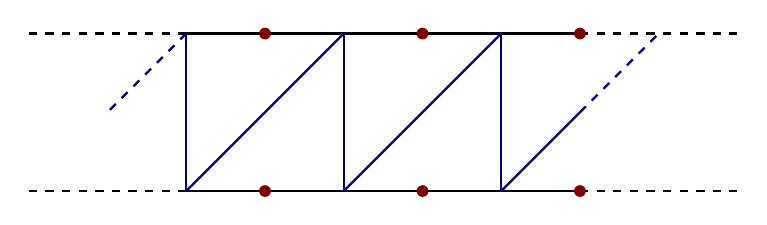
\begin{tikzpicture}
            \draw [thick] (2,2) -- (7,2);
            \draw [thick,dashed] (0,2) -- (2,2);
            \draw [thick, dashed] (7,2) -- (9,2);
            \draw [thick,dashed] (0,0) -- (2,0);
            \draw [thick,dashed] (7,0) -- (9,0);
            \draw [thick] (2,0) -- (7,0);
            \foreach \x in {3,5,7} {
                \node [circle,fill=red!50!black, inner sep=1.5pt] at (\x, 2) {};
                \node [circle,fill=red!50!black,inner sep=1.5pt] at (\x,0) {};
            }
            \draw [thick,blue!50!black] (4,0) -- (4,2);
            \draw [thick,blue!50!black] (4,0) -- (6,2);
            \draw [thick,blue!50!black] (6,2) -- (6,0);
            \draw [thick,blue!50!black] (4,2) -- (2,0);
            \draw [thick,blue!50!black] (6,0) -- (7,1);
            \draw [thick, blue!50!black,dashed] (7,1) -- (8,2);
            \draw [thick, blue!50!black] (2,0) -- (2,2);
            \draw [thick, blue!50!black, dashed] (2,2) -- (1,1);
        \end{tikzpicture}
        \caption{$\mathcal{W} (\mathbb{C}, e^z+e^{-z})$ 的生成 Lagrangian。}\label{fig:generating-Lag-equiv-P1}
    \end{figure}
    空间 $(\mathbb{C},e^z+e^{-z})$ 可如图 \ref{fig:generating-Lag-equiv-P1} 所示：红点是 $e^z+e^{-z}$ 在无穷远附近的纤维，蓝线是经指数映射 $z\mapsto e^z$ 微分同胚地投影到 $\mathbb{C}^{\ast}$ 上的 Lagrangian 子流形。我们断言，这些 Lagrangian 子流形生成包裹 Fukaya 范畴 $\mathcal{W} (\mathbb{C},e^z+e^{-z})$。\par
% [原文 p.23]
    为证明该断言，先考虑平凡 Weinstein 扇形 $X_0\coloneqq(\mathbb{C},z^2) \simeq T^{\ast} [0,1]$；此时 Weinstein 扇形 $(\mathbb{C},e^z+e^{-z})$ 可以看作把 $\mathbb{Z}$ 份 $1$-手柄按图 \ref{fig:1-handle-attaching-Z} 所示的方式粘到不交并
\[
        \bigsqcup_{\mathbb{Z}} X_0
    \]
    之上。于是显然 $\mathcal{W} (\mathbb{C},e^z+e^{-z})$ 由图 \ref{fig:1-handle-attaching-Z} 中蓝色 Lagrangian 之并生成，因为它们是扇形 $X_0$ 与各 $1$-手柄的广义余核。不难验证，这些 Lagrangian 恰好就是图 \ref{fig:generating-Lag-equiv-P1} 中所示的蓝色 Lagrangian。\par
    \begin{figure}[ht]
        \centering
        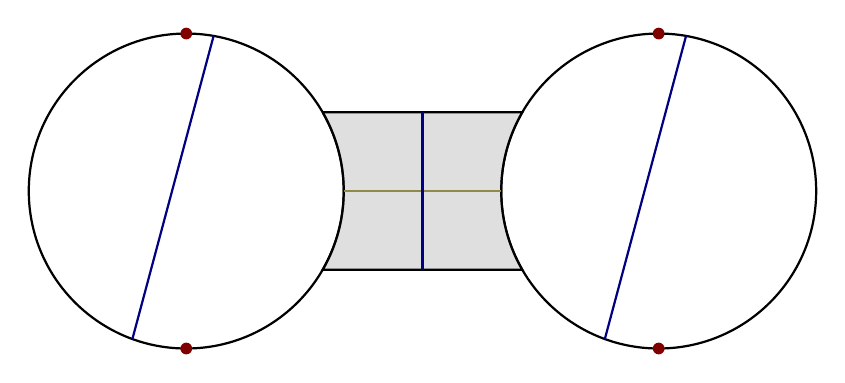
\begin{tikzpicture}
            \begin{scope}
                \draw [thick] (0,0) circle (2);
                \node [circle, fill=red!50!black, inner sep=1.5pt] at (0,2) {};
                \node [circle, fill=red!50!black, inner sep=1.5pt] at (0,-2) {};
            \end{scope}
            \begin{scope}[xshift=6cm]
                \draw [thick] (0,0) circle (2);
                \node [circle, fill=red!50!black, inner sep=1.5pt] at (0,2) {};
                \node [circle, fill=red!50!black, inner sep=1.5pt] at (0,-2) {};
            \end{scope}
            \filldraw[ fill=lightgray, fill opacity=0.5, draw=black, thick ] ({2*cos(30)},{2*sin(30)}) -- ({6+2*cos(150)},{2*sin(150)}) arc [start angle = 150, end angle = 210, radius = 2] -- ({2*cos(-30)},{2*sin(-30)}) arc [start angle = -30, end angle = 30, radius = 2];
            \draw [thick, yellow!50!black] (2,0) -- (4,0);
            \draw [thick, blue!50!black] ({2*cos(250)},{2*sin(250)}) -- ({2*cos(80)},{2*sin(80)});
            \draw [thick,blue!50!black] (3,{-2*sin(30)}) -- (3,{2*sin(30)});
            \draw [thick,blue!50!black] ({6+2*cos(250)},{2*sin(250)}) -- ({6+2*cos(80)},{2*sin(80)});
        \end{tikzpicture}
        \caption{用 $1$-手柄连接两个「标准副本」。}\label{fig:1-handle-attaching-Z}
    \end{figure}
    在计算这些 Lagrangian 的包裹 Floer 上同调之前，我们先固定一个，并把图 \ref{fig:generating-Lag-equiv-P1} 中的竖直蓝色 Lagrangian（对应图 \ref{fig:1-handle-attaching-Z} 中 $1$-手柄的余核）记作 $L_0[k]$，$k\in\mathbb{Z}$；把图 \ref{fig:generating-Lag-equiv-P1} 中的斜向 Lagrangian（对应图 \ref{fig:1-handle-attaching-Z} 中 $X_0$ 的生成 Lagrangian）记作 $L_1 [k]$。在同调镜像对称下，它们分别对应对象 $\mathcal{O}_{\mathbb{P}^1}[k]$ 与 $\mathcal{O}_{\mathbb{P}^1} (1) [k]$，其中 $k$ 是 $\mathbb{G}_m$-作用的特征。\par
    由图 \ref{fig:1-handle-attaching-Z} 显然有
\[
        CW^{\ast} (L_1[k],L_1[l])=\left\{\begin{array}{ll}
            0,&\text{若}\ l\neq k;\\
            \Bbbk,&\text{若}\ l=k.
        \end{array}\right.\quad\text{与}\quad CW^{\ast} (L_0 [k],L_0[l])=\left\{\begin{array}{ll}
            0,&\text{若}\ l\neq k;\\
            \Bbbk,&\text{若}\ l=k.
        \end{array}\right.
    \]
% [原文 p.24]
    我们约定把 $L_1[0]$ 取为 $X_0[0]$ 右侧那个 $1$-手柄里的 Lagrangian，$L_1[0]$ 就位于其中。在此约定下，同样显然有
\[
        CW^{\ast} (L_0[k],L_1 [l])=\left\{\begin{array}{ll}
            0,&\text{若}\ \vert k-l\vert\geq 2;\\
            \Bbbk,&\text{否则}.
        \end{array}\right.\quad\text{与}\quad CW^{\ast} (L_1[k],L_0[l])=0.
    \]
    于是我们完整地算出了包裹 Fukaya 范畴 $\mathcal{W} (\mathbb{C}, e^z+e^{-z})$。总结起来，$\mathcal{W} (\mathbb{C},e^z+e^{-z})$ 拟等价于无穷箭图
\[
        \begin{tikzcd}
            &\dotsb &&L_1[0] &&L_1 [1] &&\dotsb&\\
            \dotsb&&L_0[0]\arrow[ru]\arrow[lu]&&L_0[1]\arrow[ru]\arrow[lu]&&\dotsb\arrow[lu]
        \end{tikzcd}
    \]
    的路径代数上的完美模所成复形范畴。
\end{exmp}

\begin{yizhu}[特征 $k$ 的双重身份]
例中的 $k$ 同时承担两个角色：它既是 $\mathbb{Z}$-重覆盖的层数（deck 变换），又是 $\mathbb{G}_m$-作用的特征。在 B 侧它给出 $\mathcal{O}_{\mathbb{P}^1}(k)$ 的扭，在 A 侧它给出绕 $S^1$ 的单值次数，二者经同调镜像对称对应。它并不是 Floer 上同调的次数——公式里那个星号 $CW^{\ast}$ 才是同调次数，读公式时别把两者混为一谈。
\end{yizhu}

% ch06 译文：原文 §4a 后半、§4b、§4c、§4d（main.tex 第 1192--1478 行）
% 边界说明：为保持例与 figure 环境完整，本块自 p.24 上的 \begin{exmp} 起收（含整幅图 4）；
%   p.24 页首标记在前块 ch05。页首标记按 work/pagemarks/ch06.txt，仅标 p.25--p.30。
% 注：下文 tikzcd 图沿用源文的引号标签（ASCII 双引号包住 \simeq），需 tikz 的 quotes 库。
\usetikzlibrary{quotes}

\begin{exmp}\label{exmp:wrapped-Fukaya-cat-twice-punctured-equivariant}
    作为另一个例子，我们构造 Weinstein 扇形 $(\mathbb{C}\setminus\{\pm 1\},2/(1-z^2))$ 的 $\mathbb{Z}^2$-覆盖 $\mathcal{X}$。该 Weinstein 扇形可看作两个 Weinstein 扇形 $\left(\mathbb{C}^{\ast},z+z^{-1}\right)$ 沿其中一个边界停止位的扇形粘合（sectorial gluing），其 $\mathbb{Z}^2$-覆盖则可实现为每个扇形的 $\mathbb{Z}$ 个副本沿 $\mathbb{Z}^2$ 个条带粘合，如图 \ref{fig:Z2-cover-twice-punctured-disk} 所示。\par
    \begin{figure}[ht]
        \centering
        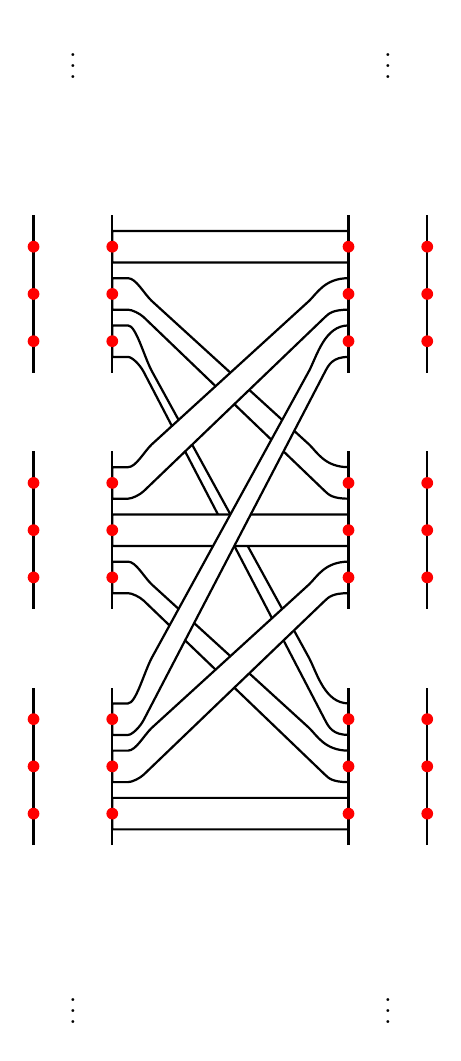
\begin{tikzpicture}       
        \begin{scope}[yshift=6cm]
            \draw [thick] (0,0) -- (0,2);
            \draw [thick] (1,0) -- (1,2);
                \foreach \x in {0.2,0.8,1.4}{
                \filldraw [fill=white, draw=black,thick] (1,\x)
            -- (1.2,\x)
            .. controls (1.25,\x)
                       and (1.35,{0.98*\x+0.02*((\x-0.2)/0.2-4.6)})
            .. (1.4,{0.96*\x+0.04*((\x-0.2)/0.2-4.6)})
            -- (3.7,{0.04*\x+0.96*((\x-0.2)/0.2-4.6)})
            .. controls (3.75,{0.02*\x+0.98*((\x-0.2)/0.2-4.6)})
                       and (3.8,{(\x-0.2)/0.2-4.6})
            .. (4,{(\x-0.2)/0.2-4.6}) -- (4,{(\x-0.2)/0.2 -4.2})
            .. controls (3.7,{(\x-0.2)/0.2-4.2}) and (3.6,{((\x-0.2)/0.2-4.2)-0.2*((\x-0.2)/0.2-4.6-\x)/2.5})
            .. (3.5,{((\x-0.2)/0.2-4.2)-0.3*((\x-0.2)/0.2-4.6-\x)/2.5})
            -- (1.5,{\x+0.4+0.3*((\x-0.2)/0.2-4.6-\x)/2.5})
            .. controls (1.4,{\x+0.4+0.2*((\x-0.2)/0.2-4.6-\x)/2.5}) and (1.3,{\x+0.4})
            ..(1.2,{\x+0.4}) -- (1,{\x+0.4}) -- cycle;
            }
            \foreach \x in {0.4,1,1.6} {
                \node [circle,fill=red,inner sep=1.5pt] at (0,\x) {};
                \node [circle,fill=red,inner sep=1.5pt] at (1,\x) {};
            }
        \end{scope}
        \begin{scope}[yshift=3cm]
            \draw [thick] (0,0) -- (0,2);
            \draw [thick] (1,0) -- (1,2);
            \foreach \x in {0.2,0.8,1.4}{
                \filldraw [fill=white, draw=black, thick] (1,\x)
            -- (1.2,\x)
            .. controls (1.25,\x)
                       and (1.35,{0.98*\x+0.02*((\x-0.2)/0.2-2.2)})
            .. (1.4,{0.96*\x+0.04*((\x-0.2)/0.2-2.2)})
            -- (3.7,{0.04*\x+0.96*((\x-0.2)/0.2-2.2)})
            .. controls (3.75,{0.02*\x+0.98*((\x-0.2)/0.2-2.2)})
                       and (3.8,{(\x-0.2)/0.2-2.2})
            .. (4,{(\x-0.2)/0.2-2.2}) -- (4,{(\x-0.2)/0.2 -1.8})
            .. controls (3.7,{(\x-0.2)/0.2-1.8}) and (3.6,{((\x-0.2)/0.2-1.8)-0.2*((\x-0.2)/0.2-2.2-\x)/2.5})
            .. (3.5,{((\x-0.2)/0.2-1.8)-0.3*((\x-0.2)/0.2-2.2-\x)/2.5})
            -- (1.5,{\x+0.4+0.3*((\x-0.2)/0.2-2.2-\x)/2.5})
            .. controls (1.4,{\x+0.4+0.2*((\x-0.2)/0.2-2.2-\x)/2.5}) and (1.3,{\x+0.4})
            ..(1.2,{\x+0.4}) -- (1,{\x+0.4}) -- cycle;
            }
            \foreach \x in {0.4,1,1.6} {
                \node [circle,fill=red,inner sep=1.5pt] at (0,\x) {};
                \node [circle,fill=red,inner sep=1.5pt] at (1,\x) {};
            }
        \end{scope}
        \begin{scope}
            \draw [thick] (0,0) -- (0,2);
            \draw [thick] (1,0) -- (1,2);
            \foreach \x in {0.2,0.8,1.4}{
                \filldraw [fill=white, draw=black,thick] (1,\x)
            -- (1.2,\x)
            .. controls (1.25,\x)
                       and (1.35,{0.98*\x+0.02*((\x-0.2)/0.2+0.2)})
            .. (1.4,{0.96*\x+0.04*((\x-0.2)/0.2+0.2)})
            -- (3.7,{0.04*\x+0.96*((\x-0.2)/0.2+0.2)})
            .. controls (3.75,{0.02*\x+0.98*((\x-0.2)/0.2+0.2)})
                       and (3.8,{(\x-0.2)/0.2+0.2})
            .. (4,{(\x-0.2)/0.2+0.2}) -- (4,{(\x-0.2)/0.2 +0.6})
            .. controls (3.7,{(\x-0.2)/0.2+0.6}) and (3.6,{((\x-0.2)/0.2+0.6)-0.2*((\x-0.2)/0.2+0.2-\x)/2.5})
            .. (3.5,{((\x-0.2)/0.2+0.6)-0.3*((\x-0.2)/0.2+0.2-\x)/2.5})
            -- (1.5,{\x+0.4+0.3*((\x-0.2)/0.2+0.2-\x)/2.5})
            .. controls (1.4,{\x+0.4+0.2*((\x-0.2)/0.2+0.2-\x)/2.5}) and (1.3,{\x+0.4})
            ..(1.2,{\x+0.4}) -- (1,{\x+0.4}) -- cycle;
            }
            \foreach \x in {0.4,1,1.6} {
                \node [circle,fill=red,inner sep=1.5pt] at (0,\x) {};
                \node [circle,fill=red,inner sep=1.5pt] at (1,\x) {};
            }
        \end{scope}
        \begin{scope}[yshift=3cm, xshift=4cm]
            \draw [thick] (0,0) -- (0,2);
            \draw [thick] (1,0) -- (1,2);
            \foreach \x in {0.4,1,1.6} {
                \node [circle,fill=red,inner sep=1.5pt] at (0,\x) {};
                \node [circle,fill=red,inner sep=1.5pt] at (1,\x) {};
            }
        \end{scope}     
        \begin{scope}[xshift=4cm]
            \draw [thick] (0,0) -- (0,2);
            \draw [thick] (1,0) -- (1,2);
            \foreach \x in {0.4,1,1.6} {
                \node [circle,fill=red,inner sep=1.5pt] at (0,\x) {};
                \node [circle,fill=red,inner sep=1.5pt] at (1,\x) {};
            }
        \end{scope}
        \begin{scope}[yshift=6cm,xshift=4cm]
            \draw [thick] (0,0) -- (0,2);
            \draw [thick] (1,0) -- (1,2);
            \foreach \x in {0.4,1,1.6} {
                \node [circle,fill=red,inner sep=1.5pt] at (0,\x) {};
                \node [circle,fill=red,inner sep=1.5pt] at (1,\x) {};
            }
        \end{scope}
        \begin{scope}[yshift=9cm]
            \node at (0.5,1) {$\vdots$};
        \end{scope}
        \begin{scope}[yshift=-3cm]
            \node at (0.5,1) {$\vdots$};
        \end{scope}
        \begin{scope}[yshift=9cm,xshift=4cm]
            \node at (0.5,1) {$\vdots$};
        \end{scope}
        \begin{scope}[yshift=-3cm,xshift=4cm]
            \node at (0.5,1) {$\vdots$};
        \end{scope}
        \end{tikzpicture}
    \caption{$\mathbb{Z}^2$-cover of the Twice-Punctured Disk with Stops.}\label{fig:Z2-cover-twice-punctured-disk}
    \end{figure}
% [原文 p.25]
    由于已知此粘合中每个扇形的生成元，对图表
\[
        \begin{tikzcd}
            \mathcal{W} \left(\bigsqcup_{\mathbb{Z}^2}T^{\ast}[0,1]\right)\arrow[r]\arrow[d]&\mathcal{W} \left(\bigsqcup_{\mathbb{Z}}(\mathbb{C},e^{z_1}+e^{-z_1})\right)\\ 
            \mathcal{W}\left(\bigsqcup_{\mathbb{Z}}(\mathbb{C},e^{z_2}+e^{-z_2})\right)&
        \end{tikzcd}
\]
应用扇形下降即可看出：$\mathcal{X}$ 仍由 Fukaya 范畴
\[\mathcal{W}\left(\bigsqcup_{\mathbb{Z}} (\mathbb{C},e^{z_i}+e^{-z_i})\right),\]
的生成元之并生成，而后者又在 $\mathbb{Z}^2$-作用下不变。\par
    基于这张粘合图表，可把 $\mathcal{W}(\mathcal{X})$ 的生成 Lagrangian 子流形标作 $L_i [a,b](c)$：其中 $i\in\{0,1\}$ 表示该 Lagrangian 来自左侧还是右侧的穿孔圆盘，$c\in\{0,1\}$ 记录 $L_i$ 的「斜率」，$(a,b)\in\mathbb{Z}^2$ 表示它位于哪个连通分支，以及在指定一个典范的 $0$ 之后它落在 $\mathbb{Z}$-覆盖的哪些叶上。\par

\begin{yizhu}[{标号 $L_i[a,b](c)$ 怎么读}]
    $i$ 记录该 Lagrangian 生于哪一个扇形（左或右侧的穿孔圆盘）；$c\in\{0,1\}$ 是它在扇形内的斜率，对应图 \ref{fig:computation-Z2-cover} 中两类不同斜率的弧；$(a,b)\in\mathbb{Z}^2$ 记录它在 $\mathbb{Z}^2$-覆盖中的位置。三个指标并不独立：沿覆盖的平移与绕中间圆周包裹的生成元一致，因此下面的 $CW^{\ast}$ 只依赖它们的差——$a_1-a_2$、$b_1-b_2$、$b_0-a_0$ 都是这种差。
\end{yizhu}

    为更好地理解 Floer 上同调 $CW^{\ast}\left(L_i [a,b](c),L_j[c,d](c);\Bbbk\right)$，观察二穿孔圆盘模型、并借助想象确定所选 Lagrangian 的提升位置更为直观，见图 \ref{fig:computation-Z2-cover}。设 $i=j$。由于绕中间圆周顺时针包裹使双次数平移 $(-1,1)$，可得
\[
    CW^{\ast}\left(L_i [a_1,b_1](c_1), L_i [a_2,b_2](c_2)\right)\simeq\left\{\begin{array}{ll}
        \Bbbk,&\text{若}\ \vert a_1 -a_2\vert\leq 1,\ b_1= b_2\ \text{且}\ c_2-c_1=1;\\
        \Bbbk,&\text{若}\ a_1-b_1=b_2-a_2\ \text{且}\ c_1=c_2;\\
        0,&\text{其他情形}.
    \end{array}\right.
\]
    \begin{figure}[ht]
        \centering
        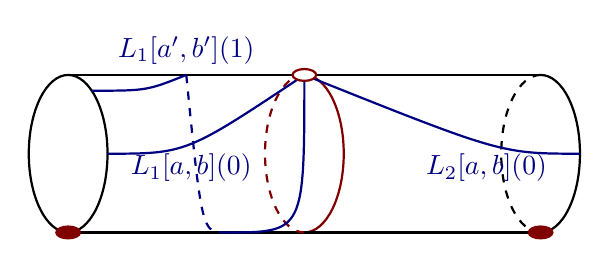
\begin{tikzpicture}
            \begin{scope}
        \draw [thick] (-2,0) arc[start angle=0, end angle=360, x radius=0.5, y radius=1];
        \draw [thick] (-2.5,1) -- (0.5,1);
        \draw [thick] (-2.5,-1) -- (0.5,-1);
        \draw [thick,red!50!black] (0.5,1) arc[start angle=90, end angle=-90, x radius=0.5, y radius=1];
        \draw [thick,red!50!black, dashed] (0.5,-1) arc[start angle=270, end angle=90, x radius=0.5, y radius=1];
        \draw [thick,blue!50!black] (-2,0) .. controls (-1,0) .. (0.5,1) node [pos=0.5,below] {$L_1[a,b](0)$};
        \draw [thick,blue!50!black] (-2.2,{sqrt(1-(0.3/0.5)^2)}) .. controls (-1.5,{sqrt(1-(0.3/0.5)^2)}) .. (-1,1) node [above] {$L_1[a',b'](1)$};
        \draw [thick,dashed,blue!50!black] (-1,1) .. controls (-0.8,-1) .. (-0.5,-1);
        \draw [thick,blue!50!black] (-0.5,-1) .. controls (0.5,-1) .. (0.5,1);
        \end{scope}
        \node [ellipse,
    minimum width=3mm,
    minimum height=1.5mm,
    inner sep=0pt,
    fill=red!50!black,
    draw=red!50!black,
    thick] at (-2.5,-1) {};
    \begin{scope}[xshift=3cm]
        \draw [thick] (-2.5,1) -- (0.5,1);
        \draw [thick] (-2.5,-1) -- (0.5,-1);
        \draw [thick] (0.5,1) arc[start angle=90, end angle=-90, x radius=0.5, y radius=1];
        \draw [thick, dashed] (0.5,-1) arc[start angle=270, end angle=90, x radius=0.5, y radius=1];
        \node [ellipse,
    minimum width=3mm,
    minimum height=1.5mm,
    inner sep=0pt,
    fill=red!50!black,
    draw=red!50!black,
    thick] at (0.5,-1) {};
    \draw [thick,blue!50!black] (1,0) .. controls (0,0) .. (-2.5,1) node [pos=0.5,below] {$L_2[a,b](0)$};
    \end{scope}
    \node [ellipse,
    minimum width=3mm,
    minimum height=1.5mm,
    inner sep=0pt,
    fill=white,
    draw=red!50!black,
    thick] at (0.5,1) {};
        \end{tikzpicture}
        \caption{Computing wrapped Floer cohomology from the base space.\label{fig:computation-Z2-cover}}
    \end{figure}
    类似地，当 $i\neq j$ 时，由图 \ref{fig:Z2-cover-twice-punctured-disk}、图 \ref{fig:computation-Z2-cover} 可读出
\[
    CW^{\ast}\left(L_i [a_0, b_0](c_i),L_j[a_1,b_1](c_j);\Bbbk\right)=\left\{\begin{array}{ll}
        \Bbbk,&\text{若}\ a_1-b_1 =b_0-a_0;\\
        0,&\text{其他情形}.
    \end{array}\right.
\]
至此我们完全刻画了包裹 Fukaya 范畴。其箭图表示（quiver presentation）将是一张三维图，此处从略。注意该空间的某种平行描述也出现在 \cite{Neumann04} 关于扩张 Bloch 群的研究中。
\end{exmp}

\begin{yizhu}[原文此处若干笔误]
    正文均照原文排印，仅在此说明：（1）标号段中「Larangian」应为 Lagrangian；（2）$CW^{\ast}\left(L_i [a,b](c),L_j[c,d](c);\Bbbk\right)$ 的第二个对象既用 $c,d$ 又把第三槽写作 $c$，与下文 $L_j[a_1,b_1](c_j)$ 的写法不一致，疑为 $L_j[a',b'](c')$；（3）全纯盘提升一段的「for some $g_i$ modulo $k$」语序混乱，译文按「$g_i$ 取某个元素、指标按模 $k$ 计」处理。
\end{yizhu}

本节最后讨论高维情形。
% [原文 p.26]
回忆：对光滑流形 $M$，在其上取 Morse 函数 $f\colon M\to\mathbb{R}$ 与 Riemann 度量 $g$，则余切丛 $T^{\ast} M$ 带有自然的 Weinstein 结构 $(\phi,\lambda_f,\omega_f)$，其中 $\phi (x,\alpha) =f(x)+\vert\alpha\vert_g^2$，$\lambda_f =df-\lambda_{\can}$，$\lambda_{\can}$ 为 $T^{\ast} M$ 上的典范 Liouville 结构，满足 $\pi^{\ast}\lambda_{\can} =\lambda_{\can}$，这里 $\pi\colon T^{\ast} M\to M$ 为丛映射，且 $\omega_f =d\lambda_f$。\par
    Legendrian 嵌入 $\Lambda\hookrightarrow\partial_{\infty} T^{\ast} M$ 给出辛超曲面 $T^{\ast}\Lambda\hookrightarrow T^{\ast} M$，后者自身带有上述 Weinstein 结构。由 \cite{Eliashberg18}，在适当修改 $T^{\ast} M$ 上的 Weinstein 结构之后，可使 $T^{\ast}\Lambda\subseteq T^{\ast} M$ 成为 Weinstein 超曲面；按 \cite{GPS20}，这便定义一个 Weinstein 扇形。\par
    一个例子出现在 \cite{FLTZ12}：取 $M=\mathbb{T}^n$，对给定的 $n$ 维多面体 $\Sigma$，可构造 Legendrian 链环 $\Lambda_{\Sigma}\hookrightarrow\partial_{\infty} T^{\ast}\mathbb{T}^n$，得到 Weinstein 扇形 $(T^{\ast}\mathbb{T}^n,\Lambda_{\Sigma})$。带拉回 Weinstein 结构的 $\mathbb{Z}^n$-覆盖 $(T^{\ast}\mathbb{R}^n,\widetilde{\Lambda}_{\Sigma})$ 按我们的定义也自然是 Weinstein 扇形。\par
    注意 $\pi_1 (T^{\ast}\mathbb{T}^n,\ast)\cong\mathbb{Z}^n$，故在 $\mathbb{Z}^n$-覆盖中 $1$-柄的粘接方式发生改变，而其余所有柄都平凡地提升。记 $X=(T^{\ast}\mathbb{R}^n,\widetilde{\Lambda}_{\Sigma})$，便可如下构造 Weinstein 配边的穷尽序列 $X_0\hookrightarrow X_1\hookrightarrow X_2\hookrightarrow\dotsb\hookrightarrow X$。\par
    $X_0$ 是有限多个点的无交并，标注为 $0$ 或 $e_i$，其中
\[
    e_i =(0,\dotsb ,0,\underbrace{1}_i,0,\dotsb ,0).
\]
$X_1$ 由 $X_0$ 粘接 $1$-柄得到：这些 $1$-柄把点 $0$ 与所有 $e_i$ 相连，所有指标更高的其余柄都位于这些 $1$-柄之上，此外还有粘接在给定柄上的半柄，它们在接触无穷远边界附近贡献 Legendrian 停止位。$X_2$ 由 $X_1$ 添加标注为 $e_i+e_j$（$1\leq i,j\leq n$）的 $0$-柄、并重复 $X_1$ 构造中所述的粘柄步骤得到。该过程可以继续，最终穷尽提升后的 Weinstein 流形 $(T^{\ast}\mathbb{R}^n,\widetilde{\Lambda}_{\Sigma})$ 的所有柄。由定义立即可得
\begin{lmm}\label{lmm:Fukaya-category-Gmn-equivariant-generation}
    包裹 Fukaya 范畴 $\mathcal{W} (T^{\ast}\mathbb{R}^n,\widehat{\Lambda}_{\Sigma})$ 由余切纤维 $T^{\ast}_q\mathbb{R}^n$（$q\in\mathbb{Z}^n$）以及无穷远处（无限型）Legendrian 链环 $\Lambda_{\Sigma}$ 的所有环绕圆盘（linking disk）生成。
\end{lmm}

\begin{yizhu}[$\widehat{\Lambda}_{\Sigma}$ 与 $\widetilde{\Lambda}_{\Sigma}$]
    引理中的 $\widehat{\Lambda}_{\Sigma}$ 与本节其余地方的 $\widetilde{\Lambda}_{\Sigma}$ 指同一对象，即 $\mathbb{Z}^n$-覆盖上的提升 FLTZ 骨架；作者在此处换了帽子的记号，当是笔误，译文照排。引理本身把「生成元」分成两族：整数点的余切纤维（对应覆盖的 $\mathbb{Z}^n$ 个基本区域）与无穷远处环绕 Legendrian 链环的圆盘（挡住 Reeb 流、使范畴成为部分包裹版本）。这正是后文能与层论一侧逐项对照的原因。
\end{yizhu}

    另一方面，由数据 $(T^{\ast}M,\Lambda)$ 可构造范畴值可构造层的 dg 范畴 $\Sh_{\Lambda} (M)$，其中层取值于 $\Bbbk$ 上链复形的 dg 范畴 \cite{GPS24M}；其奇异支撑包含在 Whitney 分层 $\mathcal{S}_{\Lambda}$ 中，而 $\mathcal{S}_{\Lambda}$ 由零截面与无穷远处 Legendrian $\Lambda$ 上的正实锥这些锥等向子流形组成。\par
    文献 \cite{GPS24M} 证明了
% [原文 p.27]
\begin{thm}[层--Floer 对应]\label{thm:sheaf-Floer-correspondence}
    设 $M$ 为光滑流形，$f\colon M\to\mathbb{R}$ 为只有有限多个临界点的 Morse 函数。则存在典范的范畴拟等价
\[
        \Perf\mathcal{W} (T^{\ast} M,\Lambda)^{op}\simeq\Sh_{\Lambda} (M)^{\omega}
\]
其中 $\Lambda$ 中一点 $p$ 处的环绕圆盘送到与 $p$ 相伴的微支撑函子（microstalk functor）的余代表元；而若 $p$ 不在 $\Lambda$ 沿投影 $\partial_{\infty} T^{\ast} M\to M$ 的像中，则余切纤维 $T^{\ast}_p M$ 送到 $p$ 处茎函子的余代表元。
\end{thm}

\begin{conceptbox}{层--Floer 对应}
    层--Floer 对应把两类看似无关的范畴等同起来：A 侧是带停止位的余切丛的包裹 Fukaya 范畴（取完美模、取 $op$ 以对齐复合方向），B 侧是底流形上奇异支撑落在该停止位之内的可构造层。对应的字典是「局部生成元 $\leftrightarrow$ 局部函子」：环绕 Legendrian 上的圆盘对应微支撑函子，底点的余切纤维对应茎函子，两者都取余代表元。它的用处是把 Floer 侧难以直接计算的生成与关系问题翻译成层论侧的局部化与粘合问题；本节正是借它在无限型扇形上把 FLTZ 情形算清楚。
\par\smallskip\noindent{\footnotesize 参考：Ganatra--Pardon--Shende, \emph{Microlocal Morse theory of wrapped Fukaya categories}, Ann. of Math. 199 (2024)；本文 §4a 的定理即引自该文。}
\end{conceptbox}

    下面我们在这一具体情形下把该定理推广到无限型扇形。
\begin{prp}\label{prp:inf-type-sheaf-Floer-Rn}
    设 $M=\mathbb{R}^n$，$\widetilde{\Lambda}_{\Sigma}$ 为提升后的 FLTZ 骨架，则 $A_{\infty}$-范畴之间存在拟等价
\[
        \Perf\mathcal{W} (T^{\ast}\mathbb{R}^n,\widetilde{\Lambda}_{\Sigma})^{op}\simeq\Sh_{\widetilde{\Lambda}_{\Sigma}} (\mathbb{R}^n)^{\omega}.
    \]
\end{prp}
\begin{proof}
    注意按构造，穷尽序列 $X_0\hookrightarrow X_1\hookrightarrow\dotsb\hookrightarrow X$ 都是带 Legendrian 停止位的余切丛给出的穷尽，因此对每个 $X_i=(T^{\ast} M_i,\Lambda_i)$，由 \cite{GPS24M} 有典范的范畴拟等价
\[
        \Perf\mathcal{W} (X_i)^{op}\simeq\Sh_{\Lambda_i} (M_i)^{\omega}.
    \]
在此拟等价下，Viterbo 函子由限制函子
\[
    \Sh_{\Lambda_{i+1}} (M_{i+1})\to\Sh_{\Lambda_i} (M_i)
    \]
实现：它把可构造层送到其在挖去若干层后的开子集上的限制；按 \cite[Lemma 4.18]{GPS24M} 的描述，该函子把紧对象送到紧对象。
    于是利用穷尽序列可直接验证，$\Sh_{\widetilde{\Lambda}_{\Sigma}} (\mathbb{R}^n)$ 可表为同伦极限
\[
        \Sh_{\widetilde{\Lambda}_{\Sigma}} (\mathbb{R}^n)\simeq\holim\left(\Sh_{\Lambda_0} (M_0)\leftarrow\Sh_{\Lambda_1} (M_1)\leftarrow\dotsb\right).
    \]
\cite[Proposition 4.20]{GPS24M} 与包裹 Fukaya 范畴的定义合起来，即给出所要的拟等价。
\end{proof}

\begin{yizhu}[无限型为何落到同伦极限]
    有限型时 $\mathcal{W}(X)$ 可由单个 Weinstein 域定义；无限型的 $X$ 只是一列 Weinstein 域 $X_0\subset X_1\subset\dotsb$ 的并，范畴只能在链层面沿 Viterbo 限制取同伦极限，这就是所谓权宜定义。证明里层论一侧写成 $\holim$、Fukaya 一侧仍写 $\mathcal{W}$，两者其实是同一件事：只有把「无限型」在两侧用同一种极限解释，逐项拟等价才能穿过极限得到整体拟等价。
\end{yizhu}

\subsection{商的包裹 Fukaya 范畴}
    设 $L,K\subseteq X/G$ 为精确柱状 spin Lagrangian 子流形，使得在 $\pi_1 (X/G)$ 中 $\langle\pi_1 (L),\pi_1 (K)\rangle\cap G= \{1\}$，则
\begin{prp}
    $CF^{\ast} (L,K) =\displaystyle\bigoplus_{g\in G} CF^{\ast} (g(\tilde{L}),\tilde{K})$ 作为分次 $\Bbbk$-模。此外，对给定的正同痕 $\psi\colon K\leadsto K^+$ 及其提升 $\tilde{\psi}$，延拓映射 $c_{\psi}\colon CF^{\ast} (L,K)\to CF^{\ast} (L,K^+)$ 与 $\displaystyle\bigoplus_{g\in G} c_{\tilde{\psi}}\colon \bigoplus_{g\in G} CF^{\ast} (g(\tilde{L}),\tilde{K})\to\bigoplus_{g\in G} CF^{\ast} (g(\tilde{L}),\tilde{K}^+)$ 一致。
\end{prp}
\begin{proof}
    $X/G$ 中的交点 $p\in L\cap K$ 对应于 $X$ 中某个 $g\in G$ 的 $\tilde{L}\cap g(\tilde{K})$ 中的点，故按 Floer 上链复形的定义有 $CF^{\ast} (L,K)=\displaystyle\bigoplus_{g\in G} (g(\tilde{L}), \tilde{K})$。给定正同痕 $\psi\colon K\leadsto K^+$ 及指定的提升 $\tilde{K}$，利用 $X\to X/G$ 是覆盖空间这一事实，可把整个同痕 $\psi$ 提升为同痕 $\tilde{\psi}\colon \tilde{K}\leadsto\tilde{K}^+$。在 $G$-作用下得到互不相交的同痕副本 $g(\tilde{\psi})\colon g(\tilde{K})\leadsto g(\tilde{K}^+)$，它们给出 Floer 理论的延拓映射
\[
        c_{g(\tilde{\psi})}\colon CF^{\ast} (g(\tilde{L}),\tilde{K})\to CF^{\ast} (g(\tilde{L}),\tilde{K}^+)
\]
% [原文 p.28]
其中 $\tilde{L}$ 取遍 $X$ 中所有选定的 Lagrangian。取直和即得所要的延拓映射。
\end{proof}
    现设 $L_0, L_1,\dotsb ,L_k$ 为 $X/G$ 中一列可容许 Lagrangian 子流形，交点为 $p_i\in CF^{\ast} (L_{i-1}, L_i)$（$1\leq i\leq k$）与 $p_0\in L_k\cap L_0$，则正则 $J$-全纯盘 $u\in\mathcal{M} (p_0;p_1,\dotsb ,p_k)$ 有唯一的自然提升
\[
\tilde{u}\in\mathcal{M}(X;\tilde{p}_0;\tilde{p}_1,\dotsb ,\tilde{p}_k)
\]
其中对 $L_i$ 选定的提升 $\tilde{L}_i$，交点 $p_i$ 提升为 $g_i (\tilde{L}_{i-1})$ 与 $\tilde{L}_i$ 的交点 $\tilde{p}_i$，$g_i$ 取某个元素、指标按模 $k$ 计；因此提升后的全纯盘 $\tilde{u}$ 贡献一个映射
\begin{multline*}
\mu^k\colon CF^{\ast} (g_{k-1}(\tilde{L}_{k-1}),\tilde{L}_k)\otimes\dotsb\otimes CF^{\ast} (g_1\dotsb g_{k-1}(\tilde{L}_0),g_2\dotsb g_{k-1} (\tilde{L}_1))\\
\to CF^{\ast} (g_1\dotsb g_k (\tilde{L}_0),\tilde{L}_k)[2-k].
\end{multline*}
反之，边界落在 $\displaystyle\bigsqcup_{g\in G}g(\tilde{L})$ 上、以交点 $g(\tilde{L}_{i-1})\cap\tilde{L}_i$ 为渐近端的任一正则 $J$-全纯盘，都投影为 $X/G$ 中边界落在 $L_i$ 上的正则 $J$-全纯盘；因此 $\mathcal{W} (X/G)$ 上的 $A_{\infty}$-结构可描述为 $\mathcal{W} (X)$ 上在 $G$-作用下不变的 $A_{\infty}$-结构。\footnote{同一论证也见于 Seidel 的工作 \cite{Seidel11}。}这足以得出定理。
\begin{proof}[定理 \ref{thm:wrapped-Fukaya-quotient} 的证明]
    由定义 \ref{defn:wrapped-Fukaya-cat-inf-sectors} 可见，包裹 Fukaya 范畴 $\mathcal{W} (X)$ 由任一 Weinstein 域穷尽序列中出现的所有余核（cocore）生成。特别地，$X$ 上 $G$-不变的 Weinstein 结构给出临界点的 $G$ 个副本，它们对应于 $X/G$ 上任一给定 Weinstein 结构的单个临界点。因此余核的无交并 $\displaystyle\bigsqcup_{g\in G} g(\tilde{L})$ 生成 $X$ 的包裹 Fukaya 范畴，其中 $\tilde{L}$ 是 $X/G$ 上 Weinstein 结构某个余核的提升。在链层面有
\[
        CW^{\ast}_{X/G}\left(L,K;\Bbbk\right)=\bigoplus_{g\in G} CW^{\ast}_X (g(\tilde{L}),\tilde{K};\Bbbk),
    \]
其中 $A_{\infty}$-结构如上述讨论所写，恰与定义 \ref{defn:Ainf-orbit-category} 中 $A_{\infty}$-轨道范畴的定义相符。
\end{proof}

\begin{yizhu}[链层面的直和其实有限]
    $G$ 可以无限（本节例子中就是 $\mathbb{Z}^2$），但 $L,K$ 紧且能量有界，只有有限多个 $g$ 使 $g(\tilde{L})$ 与 $\tilde{K}$ 相交，故直和实际上有限，不必取补全。把所有 $g$ 的副本合起来看，$\mathcal{W}(X/G)$ 的 $A_{\infty}$-结构正是 $\mathcal{W}(X)$ 上 $G$-不变的那个，这就是轨道范畴 $\mathcal{W}(X)/G$ 的链层面表述；也正因如此，商空间的问题可以完全搬到覆盖空间上逐点计算。
\end{yizhu}

\subsection{K\"unneth 定理与形变不变性}
    回忆 \cite{GPS24S} 中关于包裹 Fukaya 范畴的如下 K\"unneth 定理：
\begin{thm}[{\cite[Theorem 1.5]{GPS24S}}]\label{thm:Kunneth-theorem-Fukaya-cat}
    对有限型 Weinstein 扇形 $X$ 与 $Y$，$A_{\infty}$-范畴之间存在拟等价
\[
        \mathcal{W} (X)\otimes\mathcal{W} (Y)\simeq\mathcal{W} (X\times Y).
    \]
\end{thm}
    我们情形所需的结果略更一般：它允许 $X$ 为无限型，此时 $\mathcal{W} (X)$ 只能以权宜的方式定义。尽管如此，仍可得下述结果：
% [原文 p.29]
\begin{crl}\label{crl:Kunneth-Fukaya-infinite}
    设 $X$ 为 Weinstein 扇形，$Y$ 为另一个有限型 Weinstein 扇形，则 $A_{\infty}$-范畴之间存在拟等价
\[
        \mathcal{W} (X)\otimes\mathcal{W} (Y)\simeq\mathcal{W} (X\times Y).
    \]
\end{crl}
\begin{proof}
    设 $\emptyset=X_{-1}\subseteq X_0\subseteq\dotsb\subseteq X$ 为 $X$ 由 Weinstein 域给出的穷尽，则对每个 $n$ 有 $A_{\infty}$-范畴的拟等价
\[
        \mathcal{W} (X_n)\otimes\mathcal{W} (Y)\xrightarrow{\simeq}\mathcal{W} (X_n\times Y).
    \]
注意 Ornaghi 的张量积 \cite{Ornaghi25} 具有函子性，故 Viterbo 限制 $\mathcal{W} (X_{n+1})\twoheadrightarrow\mathcal{W} (X_n)$ 给出 $A_{\infty}$-函子
\[
        \mathcal{W} (X_{n+1})\otimes\mathcal{W} (Y)\twoheadrightarrow\mathcal{W} (X_n)\otimes\mathcal{W} (Y)
    \]
它们填入 $A_{\infty}$-范畴的同伦交换图表
\[
        \begin{tikzcd}
            \mathcal{W} (X_{n+1})\otimes \mathcal{W} (Y)\arrow[r,"\simeq"]&\mathcal{W} (X_{n+1}\times Y)\\ 
            \mathcal{W} (X_n)\otimes\mathcal{W} (Y)\arrow[u,two heads]\arrow[r,"\simeq"]&\mathcal{W} (X_n\times Y)\arrow[u,two heads]
        \end{tikzcd}
    \]
注意 $\{X_n\times Y\}_n$ 是 $X\times Y$ 由 Weinstein 子域给出的穷尽，故取同伦极限得到拟等价
\[
        \mathcal{W}^{big} (X)\otimes\mathcal{W}(Y)\simeq\mathcal{W}^{big} (X\times Y),
    \]
再对照 \ref{defn:wrapped-Fukaya-cat-inf-sectors} 的权宜定义，即得所要的 K\"unneth 同构。
\end{proof}

\begin{yizhu}[$\mathcal{W}^{big}$ 是什么]
    证明末的 $\mathcal{W}^{big}(X)$ 就是无限型扇形按穷尽序列取同伦极限所得的范畴，即 \ref{defn:wrapped-Fukaya-cat-inf-sectors} 的权宜定义；加个上标只是提醒读者这里用了极限。所以推论 \ref{crl:Kunneth-Fukaya-infinite} 虽写成一个简洁的等价式，两边其实都是同伦极限；论证的关键在于 Viterbo 限制与 K\"unneth 拟等价可交换，从而极限可以穿过张量积。
\end{yizhu}

    另一项关键要素是证明：无限型 Weinstein 扇形的某种精确辛形变不改变相应的 Fukaya 范畴。
\begin{prp}\label{prp:deformation-invariance-Fukaya}
    设 $X$ 为带 Weinstein 结构 $\phi$ 的 Weinstein 扇形，$\{\phi_t\}$ 为 Weinstein 同伦且 $\phi_0=\phi$，使得对每个 $n$，$\phi_t\vert_{X_n}$ 的零点都包含在 $X_n$ 内部的紧子集中。则 $\mathcal{W} (X,\phi_0)\simeq\mathcal{W} (X,\phi_1)$。
\end{prp}
\begin{proof}
    由 \cite{Jeffs22} 的引理 2，对每个 $n$ 有 $\mathcal{W} (X_n,\phi)\simeq\mathcal{W} (X_n,\phi_1)$；由 Weinstein 同伦的定义又可看出该拟同构与 Viterbo 限制相容。因此取同伦极限即得所要的形变不变性。
\end{proof}

\subsection{Kartal 修改}
    本节最后回忆 Kartal 修改 \cite{Kartal21}，并按当前情形作调整。设 $X$ 为有限型 Weinstein 扇形，Weinstein 结构为 $(\varphi,\lambda)$，$\phi\colon X\to X$ 为精确辛同胚，且在 $X$ 的某个柱端上为接触型；我们将构造 $(T^{\ast}\mathbb{R}\times X,e^z+e^{-z})$ 上的 Weinstein 结构 $\psi$，使 $\psi$ 在 $\tau^{-1}\times\phi$-作用下不变，其中 $\tau\colon (T^{\ast}\mathbb{R},e^z+e^{-z})\to (T^{\ast}\mathbb{R},e^z+e^{-z})$ 为平移 $1$ 的辛同胚。\par
    \cite{Kartal21} 中的拟设是考虑如下形式的 Weinstein 结构
\[
\pi_X^{\ast}\varphi_z +p^{\ast}\varphi_{(T^{\ast}\mathbb{R},e^z+e^{-z})}
\]
% [原文 p.30]
其中 $\{\varphi_z\}$ 是 $X$ 上 Weinstein 结构的 $T^{\ast}\mathbb{R}$-族，满足 $\phi^{\ast}\varphi_{z+1}=\varphi_z$；$p\colon (T^{\ast}\mathbb{R}\times X,e^z+e^{-z})\to (T^{\ast}\mathbb{R},e^z+e^{-z})$ 为到 $(T^{\ast}\mathbb{R},e^z+e^{-z})$ 因子的投影。还可进一步假设 $\varphi_{z=x+iy}$ 关于 $y$ 不变，且在 $x\in\mathbb{Z}$ 时为常值；于是所得 Weinstein 形变不改变停止位，可直接记作 $\{\varphi_s\}_{s\in\mathbb{R}}$。由 $\phi$ 的定义可取光滑函数 $K\colon X\to\mathbb{R}$，使 $\phi^{\ast}\lambda_X=\lambda_X+dK$；$\{\lambda_s\}$ 的构造则取一族在 $X$ 的柱端上呈柱状的光滑函数 $\{K_s\}_{s\in\mathbb{R}}$，使 $\lambda_s =\lambda +dK_s$。条件 $\phi^{\ast}\lambda_{s+1}=\lambda_s$ 于是化为
\[
    dK_s=d(\phi^{\ast} K_{s+1}+K).
\]
按 \cite{Kartal21} 命题 2.1 证明中完全相同的步骤，可找到光滑函数族 $K_s$，使 $\phi^{\ast} K_{s+1} +K-K_s=0$ 对所有 $s\in\mathbb{R}$ 成立。\par
    要把该 Liouville 结构提升为 Weinstein 结构，还需选取光滑函数族 $\varphi_s$ 与常数 $C>0$，使 $\varphi_C =p^{\ast}\varphi_{(T^{\ast}\mathbb{R},e^z+e^{-z})} +C^{-1}\varphi_z$ 成为 Liouville 结构 $\lambda_C =p^{\ast}\lambda_{(T^{\ast}\mathbb{R},e^z+e^{-z})} +C^{-1}\lambda_z$ 的 Lyapunov 函数。\cite{Kartal21} 中的结论于是为
\begin{prp}[{与 \cite{Kartal21} 命题 2.3 类似}]\label{prp:Kartal-modification-Weinstein}
    $(T^{\ast}\mathbb{R}\times X,e^z+e^{-z})$ 上存在形如
\[
        \varphi_{(T^{\ast}\mathbb{R}\times X,e^z+e^{-z})} =p^{\ast}\varphi_{(T^{\ast}\mathbb{R},e^z+e^{-z})}+C^{-1}\varphi_z,\quad \lambda_{(T^{\ast}\mathbb{R}\times X,e^z+e^{-z})}=\pi^{\ast}\lambda_{(T^{\ast}\mathbb{R},e^z+e^{-z})} +C^{-1}\lambda_z
    \]
的 Weinstein 结构（$C>0$ 充分大），且该结构在 $(T^{\ast}\mathbb{R}\times X,e^z+e^{-z})$ 的 $\tau^{-1}\times\phi$-作用下不变。
\end{prp}

\begin{conceptbox}{Kartal 修改}
    Kartal 修改把「带单值性的映射柱」从一族辛流形的极限做成一个真正的 Weinstein 扇形。做法是在 $T^{\ast}\mathbb{R}\times X$ 上取 Weinstein 结构 $\pi_X^{\ast}\varphi_z+p^{\ast}\varphi_{(T^{\ast}\mathbb{R},e^z+e^{-z})}$，其中 $\{\varphi_z\}$ 满足 $\phi^{\ast}\varphi_{z+1}=\varphi_z$——这条协变条件让「沿 $\mathbb{R}$ 方向平移 $1$ 并同时作用 $\phi$」成为结构的对称，于是 $\tau^{-1}\times\phi$ 自动是辛同胚。$T^{\ast}\mathbb{R}$ 方向两端的 $e^z$、$e^{-z}$ 给出两个停止位，把本来会逃到无穷远的 Reeb 流挡住；$C$ 取得足够大则保证修改后仍有 Lyapunov 函数。它的意义是：映射柱上的包裹 Fukaya 范畴因此可以按 §4b 的商范畴技术计算，这为后文把射影丛的 A 模型归约到 $\mathcal{W}(X)$ 与 $\phi$ 的轨道范畴提供了舞台。
\par\smallskip\noindent{\footnotesize 参考：Kartal, \emph{Distinguishing open symplectic mapping tori via their wrapped Fukaya categories}, Geom. Topol. 25 (2021), §2；本文 \cite{Kartal21}。}
\end{conceptbox}

\begin{keytakeaways}
    \item 目标：把商空间 $X/G$ 的包裹 Fukaya 范畴归约为 $X$ 上 $G$-等变的结构，即 $\mathcal{W}(X/G)\simeq\mathcal{W}(X)/G\simeq\mathcal{W}(X)_G$（取扭完备之后，定理 \ref{thm:wrapped-Fukaya-quotient}）。证明的要点是全纯盘、同痕与余核都能逐层提升，链层面 $CW^{\ast}_{X/G}=\bigoplus_{g}CW^{\ast}_X$，与 $A_{\infty}$-轨道范畴的定义对齐。
    \item 例子：二穿孔圆盘的 $\mathbb{Z}^2$-覆盖（例 \ref{exmp:wrapped-Fukaya-cat-twice-punctured-equivariant}）用扇形粘合与两张图给出显式的 $CW^{\ast}$——$i=j$ 时由双次数平移决定，$i\neq j$ 时只看斜率之差；这类计算是后文对照 A、B 两侧的原料。
    \item 高维情形：$\mathbb{Z}^n$-覆盖的 FLTZ 扇形借穷尽序列与层--Floer 对应（定理 \ref{thm:sheaf-Floer-correspondence}、命题 \ref{prp:inf-type-sheaf-Floer-Rn}）化为 $\Sh_{\widetilde{\Lambda}_{\Sigma}}(\mathbb{R}^n)$ 的同伦极限，把无限型的 Fukaya 范畴变成可算的层论对象。
    \item 工具：K\"unneth 定理（定理 \ref{thm:Kunneth-theorem-Fukaya-cat}、推论 \ref{crl:Kunneth-Fukaya-infinite}）与形变不变性（命题 \ref{prp:deformation-invariance-Fukaya}）允许对乘积与精确辛形变自由操作；Kartal 修改（命题 \ref{prp:Kartal-modification-Weinstein}）则把带单值性的映射柱做成正规的 Weinstein 扇形。
\end{keytakeaways}

% ch07 译文：原文 §5a（main.tex 第 1805–2169 行）
\section{$G$-等变层\label{sec:G-equiv-sheaves}}
本节回顾 $G$-等变层的定义（可参看 \cite[\href{https://stacks.math.columbia.edu/tag/03LE}{Tag 03LE}]{stacks-project}），并建立概形 $X$ 上 $G$-等变凝聚层与向量丛同 $X$ 上 $H$-等变凝聚层与向量丛之间的关系，其中 $H\subseteq G$ 为子群。

\subsection{$G$-等变 $\mathcal{O}_X$-模的范畴}

设 $G=(G, m, e)$ 为 $\field$ 上的群概形，乘法为 $m : G \times G \rightarrow G$，单位截面为 $e : \Spec(\field) \rightarrow G$；设 $X$ 为 $\field$ 上的概形，带有 $G$-作用 $\sigma : G \times X \rightarrow X$。若干基本定义见 \cite[\href{https://stacks.math.columbia.edu/tag/022R}{Section 022R}]{stacks-project} 与 \cite[\href{https://stacks.math.columbia.edu/tag/01II}{Section 01II}]{stacks-project}。

\begin{defn}\label{defn:EquivariantSheaves}
一个\emph{$G$-等变 $\mathcal{O}_X$-模}
$(\mathcal{F}, \theta)$
指一个 $\mathcal{O}_X$-模 $\mathcal{F}$，连同 $\mathcal{O}_{G\times X}$-模的同构
$$
\theta : \sigma^* \mathcal{F} \xrightarrow{\cong} \left(\pr_X^{G \times X}\right)^* \mathcal{F}
$$
（称为 $\mathcal{F}$ 的\emph{$G$-线性化}），其中 $\pr_X^{G \times X} : G \times X \rightarrow X$ 为自然投影，并且下列条件成立：
% [原文 p.31]
\begin{itemize}
\item \emph{（余循环条件）}
$
(m \times \id_X)^* \theta
=
(\id_G \times \sigma)^* \theta \comp \left(\pr_{G \times X}^{G \times G \times X}\right)^* \theta.
$

\item \emph{（单位条件）}
$(e \times \id_X)^*\theta = \id_{\mathcal{F}}$.
\end{itemize}

从\emph{$G$-等变 $\mathcal{O}_X$-模}
$\mathcal{F}=(\mathcal{F}, \theta)$
到
$\mathcal{F}'=(\mathcal{F}', \theta')$
的\emph{态射}，指一个 $\mathcal{O}_X$-模态射
$
f : \mathcal{F} \rightarrow \mathcal{F}'
$
，它与 $G$-线性化交换，即
$$
\sigma^* f \comp \theta'
=
\theta \comp \left(\pr_X^{G \times X}\right)^* f
$$
作为 $\mathcal{O}_{G \times X}$-模的态射成立。

我们把\emph{$G$-等变 $\mathcal{O}_X$-模的范畴}记作
$\Mod_G(X)$。
若 $(\mathcal{F},\theta)$ 底下的 $\mathcal{F}$ 作为 $\mathcal{O}_X$-模具有相应性质，就说 $G$-等变 $\mathcal{O}_X$-模 $(\mathcal{F},\theta)$ 是
\emph{拟凝聚}、\emph{凝聚}
或\emph{有限秩局部自由}的。以 $G$-等变拟凝聚、凝聚、有限秩局部自由的 $\mathcal{O}_X$-模为对象，$\Mod_G(X)$ 有三个满子范畴，分别记作
$\QCoh_G(X)$、
$\Coh_G(X)$、
$\VB_G(X)$，
它们满足
$$
\VB_G(X)\subset\Coh_G(X)\subset\QCoh_G(X)\subset\Mod_G(X).
$$
\end{defn}

\begin{conceptbox}{$G$-等变层}
$G$-等变层（\emph{$G$-equivariant sheaf}）就是叠加了「沿群作用的函子性」的层：$G$-线性化 $\theta:\sigma^*\mathcal{F}\xrightarrow{\cong}\left(\pr_X^{G\times X}\right)^*\mathcal{F}$ 把「先作用再取层」与「先取层再作用」两种拉回等同起来，余循环条件保证该等同在 $G\times G\times X$ 上相容，单位条件则让单位截面处的等同退化为恒等。它等价于商叠 $[X/G]$ 上的拟凝聚层，因而是「带 $G$-作用的空间上的层」的正确范畴化：普通层只记得 $X$ 的局部结构，等变层额外记住每点沿 $G$-轨道的平移。本文需要它，是因为 B 侧的 $\mathbb{G}_m$-主丛 $L(Y,\xi)^{\times}\to Y$ 上的层正是 $Y$ 上的 $\mathbb{G}_m$-等变层，而等变层按权分解（见 §5c）恰好与 A 侧绕 $\mathbb{P}^1$ 纤维方向的单值性、停止位选择相对应。
\par\smallskip\noindent{\footnotesize 参考：nLab，\emph{equivariant sheaf}；Stacks Project，Tag 03LE。}
\end{conceptbox}

\begin{yizhu}[$\Theta$ 的共轭方向]
内部 Hom 的线性化取共轭 $\Theta:\alpha\mapsto\theta^{-1}\comp\alpha\comp\theta'$，两头方向相反：源侧用 $\theta^{-1}$ 把 $\sigma^*\mathcal{F}$ 拉回 $\left(\pr_X^{G\times X}\right)^*\mathcal{F}$，靶侧用 $\theta'$ 把 $\sigma^*\mathcal{F}'$ 送到 $\left(\pr_X^{G\times X}\right)^*\mathcal{F}'$。若误写成 $\theta\comp\alpha\comp\theta'^{-1}$，得到的共轭与原意相反，§5c 中权 $\cha$ 会整体变号。还要注意本节证明里出现的 $\cdot$ 有时表示复合而非数乘，如下面命题证明中的 $\theta_U^{-1}\cdot\sigma_U^*f\cdot\theta'_U$。
\end{yizhu}

\begin{defn}[等变层的内部张量积]
\label{defn:TensorProductOfEquivariantModules}
设 $(\mathcal{F}, \theta)$ 与 $(\mathcal{F}', \theta')$ 为 $\Mod_G(X)$ 中的两个 $G$-等变 $\mathcal{O}_X$-模。
$(\mathcal{F}, \theta)$ 与 $(\mathcal{F}', \theta')$ 的\emph{（内部）张量积}
$$
(\mathcal{F}, \theta)
\underset{\mathcal{O}_X}{\otimes}
(\mathcal{F}', \theta')
:=
\left(\mathcal{F}\underset{\mathcal{O}_X}{\otimes}\mathcal{F}', \, \theta\otimes\theta'\right)
\in
\Mod_G(X),
$$
定义为 $\mathcal{O}_X$-模 $\mathcal{F}\underset{\mathcal{O}_X}{\otimes}\mathcal{F}'$
连同 $G$-线性化
$$
\theta\otimes\theta'
:
\sigma^*\left(
\mathcal{F}
\underset{\mathcal{O}_X}{\otimes}
\mathcal{F}'
\right)
\xrightarrow{\cong}
\left(\pr_X^{G \times X}\right)^*
\left(\mathcal{F}
\underset{\mathcal{O}_X}{\otimes}
\mathcal{F}'\right)
$$
给出，后者是张量积 $\theta \otimes \theta'$ 在典范同构
$$
\begin{gathered}
\sigma^*\left(\mathcal{F}\underset{\mathcal{O}_X}{\otimes}\mathcal{F}'\right)
\cong
\sigma^* \mathcal{F} \underset{\mathcal{O}_{G \times X}}{\otimes} \sigma^* \mathcal{F}' \\
\text{与}\quad
\left(\pr_X^{G \times X}\right)^* \left(\mathcal{F}\underset{\mathcal{O}_X}{\otimes}\mathcal{F}'\right)
\cong
\left(\pr_X^{G \times X}\right)^*\mathcal{F} \underset{\mathcal{O}_{G \times X}}{\otimes} \left(\pr_X^{G \times X}\right)^*\mathcal{F}'
\end{gathered}
$$
之下的像。

张量积的\emph{单位对象}定义为
$(\mathcal{O}_X, \id_{\mathcal{O}_{G\times X}}) \in \Mod_G(X)$，
其中
$
\id_{\mathcal{O}_{G\times X}}
:
\sigma^* \mathcal{O}_X
\xrightarrow{\cong}
\left(\pr_X^{G \times X}\right)^* \mathcal{O}_X
$
由层的典范同构
$
\sigma^* \mathcal{O}_X
\cong
\mathcal{O}_{G\times X}
$
与
$
\left(\pr_X^{G \times X}\right)^* \mathcal{O}_X
\cong
\mathcal{O}_{G\times X}
$
诱导得到。

配备该张量积，
$\Mod_G(X)$
构成一个
\emph{对称幺半范畴}
$
\left(
\Mod_G(X),
\underset{\mathcal{O}_X}{\otimes},
\left(\mathcal{O}_X,\theta(0)\right)
\right).
$
此外，$\underset{\mathcal{O}_X}{\otimes}$ 限制下去，也赋予
$\QCoh_G(X)$、$\Coh_G(X)$、$\VB_G(X)$
对称幺半范畴结构。

\end{defn}

\begin{yizhu}[单位对象为何写成 $\theta(0)$]
本定义的开头把张量积的单位对象写成 $(\mathcal{O}_X,\id_{\mathcal{O}_{G\times X}})$，末尾的对称幺半范畴却写成 $\left(\mathcal{O}_X,\theta(0)\right)$：两处指的是同一个线性化，$\theta(0)$ 应理解为「未用任何特征扭过的恒等线性化」，即上面由 $\sigma^*\mathcal{O}_X\cong\mathcal{O}_{G\times X}\cong\left(\pr_X^{G\times X}\right)^*\mathcal{O}_X$ 诱导的那一个。原文记号不统一，读时按平凡线性化处理即可；§5b 的扭构造正是在这个 $\theta(0)$ 上乘以特征。
\end{yizhu}

\begin{defn}[等变层的内部 Hom]
\label{defn:InternalHomOfEquivariantModules}
设 $(\mathcal{F}, \theta)$ 与 $(\mathcal{F}', \theta')$ 为 $\Mod_G(X)$ 中的两个 $G$-等变 $\mathcal{O}_X$-模，
且 $\mathcal{F}$ 有限表现\footnote{
$\mathcal{O}_X$-模 $\mathcal{F}\in\Mod(X)$
称为有限表现，若
(1)
$\mathcal{F}\in\VB(X)$ 为有限秩局部自由，
或
(2)
$X$ 局部 Noether 且 $\mathcal{F}\in\Coh(X)$ 为凝聚层。
}。
$(\mathcal{F}, \theta)$ 与 $(\mathcal{F}', \theta')$ 的\emph{内部 Hom}
$$
\mathcal{H}om_{\mathcal{O}_X}\left( (\mathcal{F}, \theta), (\mathcal{F}', \theta') \right)
:=
\left( \mathcal{H}om_{\mathcal{O}_X}(\mathcal{F}, \mathcal{F}'), \, \Theta \right)
\in
\Mod_G(X),
$$
定义为 $\mathcal{O}_X$-模 $\mathcal{H}om_{\mathcal{O}_X}(\mathcal{F}, \mathcal{F}')$
连同 $G$-线性化
$$
\Theta
:
\sigma^*\mathcal{H}om_{\mathcal{O}_X}(\mathcal{F}, \mathcal{F}')
\xrightarrow{\cong}
\left(\pr_X^{G \times X}\right)^* \mathcal{H}om_{\mathcal{O}_X}(\mathcal{F}, \mathcal{F}')
$$
给出，后者由共轭
$
\alpha
\mapsto
\theta^{-1}
\comp
\alpha
\comp
\theta'
$
在典范同构\footnote{
这些典范同态是同构，因为态射
$\sigma$、
$\pr_X^{G\times X}
:
G \times X \rightarrow X$
都平坦（任何群概形 $G$ 对基平坦），
且 $\mathcal{F}$ 有限表现。
}
之下给出
% [原文 p.32]
\begin{align*}
\sigma^* \mathcal{H}om_{\mathcal{O}_X}(\mathcal{F}, \mathcal{F}')
&\xrightarrow{\cong}
\mathcal{H}om_{\mathcal{O}_{G \times X}}\left(\sigma^* \mathcal{F}, \sigma^* \mathcal{F}'\right)
\quad\text{与}\quad
\\[2mm]
\left(\pr_X^{G \times X}\right)^* \mathcal{H}om_{\mathcal{O}_X}(\mathcal{F}, \mathcal{F}')
&\xrightarrow{\cong}
\mathcal{H}om_{\mathcal{O}_{G \times X}}\left(\left(\pr_X^{G \times X}\right)^*\mathcal{F}, \left(\pr_X^{G \times X}\right)^*\mathcal{F}'\right).
\end{align*}

更确切地说，对每个开集 $U \subseteq G \times X$ 与局部截面
$
\alpha \in \left(\sigma^*\mathcal{H}om_{\mathcal{O}_X}(\mathcal{F}, \mathcal{F}')\right)(U)
$，
把它看作 $\mathcal{O}_{G\times X}|_U$-模同态
$
\alpha : \sigma^*\mathcal{F}|_U \rightarrow \sigma^*\mathcal{F}'|_U
$，
截面 $\Theta(U)(\alpha)$ 由复合
$$
\left(\theta|_U\right)^{-1}
\comp
\alpha
\comp
\theta'|_U
:
\left(\pr_X^{G \times X}\right)^*\mathcal{F}|_U
\rightarrow
\left(\pr_X^{G \times X}\right)^*\mathcal{F}'|_U
$$
定义。

配备张量积与内部 Hom 后，
$\VB_G(X)$
（以及当 $X$ 局部 Noether 时的 $\Coh_G(X)$）
构成一个\emph{闭对称幺半范畴}。

\end{defn}

\begin{yizhu}[内部 Hom 为何要假设有限表现]
把 $\mathcal{H}om$ 搬过拉回需要两个条件：$\sigma$ 与 $\pr_X^{G\times X}$ 平坦（群概形对基平坦，这一条自动成立），以及 $\mathcal{F}$ 有限表现。缺了后者，$\sigma^*\mathcal{H}om(\mathcal{F},\mathcal{F}')$ 与 $\mathcal{H}om(\sigma^*\mathcal{F},\sigma^*\mathcal{F}')$ 只是同态而非同构，$\Theta$ 便无法定义成线性化。原文用两条脚注把这两处补上；读时注意「有限表现」在局部 Noether 情形下就是凝聚，而在一般概形上则要单独假设。
\end{yizhu}

本段最后，我们计算 $G$-等变层之间的截面。
\begin{prop}\label{prop:InvariantSectionsOfEquivariantInternalHom}
设
$(\mathcal H,\Theta)
:=
\mathcal Hom_{\mathcal O_X}
\bigl((\mathcal F,\theta),(\mathcal F',\theta')\bigr)$。
则对每个 $G$-不变开子概形 $U\subseteq X$，有
$$
\mathcal H(U)^G
=
\Hom_{\Mod_G(U)}
\left(
(\mathcal F,\theta)|_U,\,
(\mathcal F',\theta')|_U
\right).
$$
\end{prop}

\begin{proof}
截面 $f\in\mathcal H(U)$ 是 $\mathcal O_U$-模态射 $f:\mathcal F|_U\rightarrow\mathcal F'|_U$。
由 $G$-不变截面的定义与 $\Theta$ 的定义，下列等价成立：
\begin{align*}
f\in\mathcal H(U)^G
&\quad\Leftrightarrow\quad
\Theta|_{G\times U}(\sigma_U^*f)
=
\left(\pr_U^{G\times U}\right)^*f
\\
&\quad\Leftrightarrow\quad
\theta_U^{-1}\cdot\sigma_U^*f\cdot\theta'_U
=
\left(\pr_U^{G\times U}\right)^*f
\\
&\quad\Leftrightarrow\quad
\sigma_U^*f\cdot\theta'_U
=
\theta_U\cdot
\left(\pr_U^{G\times U}\right)^*f
\end{align*}
最后一个等式恰是 $f$ 的 $G$-等变性条件。
\end{proof}

% ch08 译文：原文 §5b–§5c（main.tex 第 2170–2670 行）
\subsection{特征群 $\widehat{G}$ 在 $\Mod_G(X)$ 上的作用}

在 $X$ 上 $G$-等变层构成的 Abel 范畴 $\Mod_G(X)$ 中，有一个特定的 Abel 群 $\widehat{G}$ 的典范作用；$\widehat{G}$ 称为 $G$ 的\emph{特征群}（character group），下面给出定义。

\begin{defn}
% [原文 p.33]
群概形 $(G,m,e)$ 的\emph{特征}（\emph{character}）指从 $G$ 到乘法群概形
$
\Gm := \Spec\left(\field[t, t^{-1}]\right)
$
的群概形同态
$
\cha : G \longrightarrow \Gm
$。
等价地，特征对应于平凡 $\Gm$-丛 $\mathcal{O}_G^\times$ 在 $G$ 上的一个整体截面
$
\cha
\in
\Gamma\left(G, \mathcal{O}_G^\times\right)
$，
满足
$$
m^* \cha
=
\left(\pr_{G,1}^{G \times G}\right)^* \cha
\cdot
\left(\pr_{G,2}^{G \times G}\right)^* \cha
\in
\Gamma\left(G \times G, \mathcal{O}_{G \times G}^\times\right),
$$
其中
$\pr_{G,1}^{G \times G}$、
$\pr_{G,2}^{G \times G}
:
G \times G \rightarrow G
$
分别为到第一、第二因子的投影，
$
\left(\pr_{G,i}^{G \times G}\right)^* \cha
\in
\Gamma\left(
G \times G,
\left(\pr_{G,i}^{G \times G}\right)^*\mathcal{O}_G^\times
\cong
\mathcal{O}_{G \times G}^\times
\right)
$
是 $\cha$ 沿 $\pr_{G,i}^{G\times G}$ 的拉回（$i\in\{1,2\}$），而 $\cdot$ 表示环
$\mathcal{O}_{G\times G}^\times(G\times G)$ 中元素的乘法。

$G$ 的所有特征构成一个 Abel 群，其群结构由 $\Gm$ 的乘法群概形结构诱导，记作
$$
\widehat{G}
:=
\operatorname{Hom}_{\mathsf{GrpSch}(\field)}\left(G, \Gm\right),
$$
并称为 $G$ 的\emph{特征群}（\emph{character group}）。
\end{defn}

\begin{yizhu}[「特征」的两种等价说法]
特征既可以看成群概形同态 $\cha:G\rightarrow\Gm$，也可以看成 $\Gamma(G,\mathcal{O}_G^\times)$ 中满足 $m^*\cha=(\pr_{G,1})^*\cha\cdot(\pr_{G,2})^*\cha$ 的可逆整体截面：前者由 $\Gm$ 的泛性质与 $\Gm=\Spec(\field[t,t^{-1}])$ 的坐标环决定，后者正是把该同态写成「$t\mapsto\cha$」后的样子。乘法条件保证 $\cha(gh)=\cha(g)\cha(h)$，所以全体特征在逐点相乘下构成 Abel 群 $\widehat{G}$。后文把 $\cha$ 同时当作「群同态」与「可逆截面」使用，正是靠这一等同；$\widehat{G}$ 交换这一事实，则是 §5c 中权空间分解能按特征标逐项拆开的根本原因。

另需说明：原文此处把该丛误写作「the trivial $\Gm$-bundle $\mathcal{O}_X^\times$ on $X$」，但紧接着的公式写的是 $\Gamma(G,\mathcal{O}_G^\times)$ 与 $\mathcal{O}_{G\times G}^\times$，可见所论丛应是 $G$ 上的 $\mathcal{O}_G^\times$；译文按此处理。
\end{yizhu}

\begin{defn}[按特征作扭]
对每个特征
$\cha \in \widehat{G}\subset\Gamma\left(G, \mathcal{O}_G^\times\right)$，
\emph{按 $\cha$ 扭过的平凡线丛}定义为
$$
\mathcal{O}_X(\cha)
:=
(\mathcal{O}_X, \id_{\mathcal{O}_{G\times X}}(\cha))
\in \vb_G(X),
$$
其中底下的 $\mathcal{O}_X$-模是 $\mathcal{O}_X$，$G$-线性化
$$
\id_{\mathcal{O}_{G\times X}}(\cha)
:=
\left(\pr_G^{G \times X}\right)^* \cha \cdot \id_{\mathcal{O}_{G\times X}}
:
\mathcal{O}_{G\times X}
\xrightarrow{\cong}
\mathcal{O}_{G\times X}
$$
（在典范同构
$
\sigma^* \mathcal{O}_X
\cong
\mathcal{O}_{G\times X}
$
与
$
\left(\pr_X^{G \times X}\right)^* \mathcal{O}_X
\cong
\mathcal{O}_{G\times X}
$
之下）由 $\cha$ 沿自然投影
$\pr_G^{G\times X}:G\times X\rightarrow G$ 的拉回
$$
\left(\pr_G^{G \times X}\right)^* \cha
\in
\Gamma\left(G \times X, \left(\pr_G^{G\times X}\right)^*\mathcal{O}_G^\times \cong \mathcal{O}_{G \times X}^\times\right)
$$
与恒等线性化的乘法定义。更确切地说，对每个开集
$U\subseteq G\times X$
与
$s\in\mathcal{O}_{G\times X}(U)$，
定义
$$
\left(\left(\id_{\mathcal{O}_{G\times X}}(\cha)\right)(U)\right)(s)
:=
\left(\left.\left(\pr_G^{G \times X}\right)^* \cha\right|_U\right)
\cdot
s
\in
\mathcal{O}_{G\times X}(U),
$$
其中 $\cdot$ 表示环
$\mathcal{O}_{G\times X}(U)$ 中元素的乘法。

设 $(\mathcal{F}, \theta)$ 为 $\Mod_G(X)$ 中的 $G$-等变 $\mathcal{O}_X$-模，$\cha \in \widehat{G}$。
$(\mathcal{F},\theta)$ \emph{按 $\cha$ 的扭}定义为
$$
(\mathcal{F},\theta)(\cha)
:=
(\mathcal{F}, \theta(\cha))
\in \Mod_G(X),
$$
其中底下的 $\mathcal{O}_X$-模是 $\mathcal{F}$，$G$-线性化
$$
\theta(\cha)
:=
\left(\pr_G^{G \times X}\right)^* \cha \cdot \theta
:
\sigma^* \mathcal{F}
\xrightarrow{\cong}
\left(\pr_X^{G \times X}\right)^* \mathcal{F}
$$
由 $\cha$ 沿自然投影 $\pr_G^{G\times X}$ 的拉回
$$
\left(\pr_G^{G \times X}\right)^* \cha
\in
\Gamma\left(G \times X, \left(\pr_G^{G\times X}\right)^*\mathcal{O}_G^\times \cong \mathcal{O}_{G \times X}^\times\right)
$$
对原 $G$-线性化 $\theta$ 的数乘定义。更确切地说，对每个开集
$U\subseteq G\times X$
与
$s\in(\sigma^*\mathcal{F})(U)$，
定义
$$
(\theta_{\cha}(U))(s)
:=
\left(\left.\left(\pr_G^{G \times X}\right)^* \cha\right|_U\right)
\cdot
(\theta(U)(s))
\in
\left(\left(\pr_X^{G \times X}\right)^*\mathcal{F}\right)(U),
$$
其中 $\cdot$ 表示 $\mathcal{O}_{G\times X}(U)$ 中元素对 $\mathcal{O}_{G\times X}(U)$-模
$\left(\left(\pr_X^{G \times X}\right)^*\mathcal{F}\right)(U)$ 中元素的数乘。

按特征作扭定义了 $\Mod_G(X)$ 上的一个严格 $\widehat{G}$-作用（strict $\widehat{G}$-action）
$$
\phi:\widehat{G}\rightarrow\Aut_{\str}(\Mod_G(X)),
\quad
\cha\mapsto \phi_{\cha},
$$
其中
$$
\phi_{\cha}:\Mod_G(X)\rightarrow\Mod_G(X),
\quad
(\mathcal{F},\theta)
\mapsto
(\mathcal{F},\theta(\cha)).
$$
% [原文 p.34]
这限制为 $\QCoh_G(X)$、$\Coh_G(X)$ 与 $\VB_G(X)$ 上的严格 $\widehat{G}$-作用。
\end{defn}

\begin{rmk}
存在自然同构
$$
(\mathcal{F},\theta)(\cha)
\cong
(\mathcal{F},\theta)
\underset{\mathcal{O}_X}{\otimes}
\mathcal{O}_X(\cha)
\in\Mod_G(X).
$$
\end{rmk}

\subsection{权空间分解}

由于 $\widehat{G}$ 交换，它在 $\Mod_G(X)$ 中同态空间上的作用会把同态空间分解为一维不可约 $\widehat{G}$-表示的直和；我们称之为\emph{权空间分解}（weight space decomposition）。

\begin{conceptbox}{权空间分解}
权空间分解是「交换群作用在向量空间上必可对角化」这一线性代数事实在层论中的推广：当群是对角化群概形 $G=\Spec(\field[\Lambda])$ 时，$\Mod_G(X)$ 中每个对象的整体截面都带 $\field[\widehat{G}]$ 的余模结构（即 $\widehat{G}$-分次结构），于是按特征标 $\cha\in\widehat{G}$ 拆成直和 $\mathcal{F}(X)=\bigoplus_{\cha}\mathcal{F}(X)_{\cha}$，每个 $\mathcal{F}(X)_{\cha}$ 就是「权为 $\cha$ 的部分」。更关键的是，Hom 空间本身也按权分解，且权 $\cha$ 的那一块恰是 $\Hom_{\Mod_G(X)}((\mathcal{F},\theta)(\cha),(\mathcal{F}',\theta'))$ —— 即「把源扭过 $\cha$ 之后」的等变同态。本文 B 侧正是靠这一分解，把 $\mathbb{P}^1$ 上 $\mathbb{G}_m$-等变层的同态空间按权拆开，从而与 A 侧绕 $S^1$ 的单值性、停止位选择逐项对应；§5c 的推论把这一分解提升为轨道范畴的全忠实嵌入，是证明主定理的重要中间步骤，也是 §6 扭 Künneth 公式的技术核心。
\par\smallskip\noindent{\footnotesize 参考：nLab，\emph{equivariant sheaf}；本文 §5b–§5c、§6。}
\end{conceptbox}

\begin{defn}
设 $\Lambda$ 为 Abel 群，$\field$ 为交换环。
\emph{群代数}（\emph{group algebra}）$\field[\Lambda]$ 是一个以 $\{e_\lambda\}_{\lambda \in \Lambda}$ 为基的 Hopf 代数，其中余乘法 $\Delta : \field[\Lambda] \rightarrow \field[\Lambda] \underset{\field}{\otimes} \field[\Lambda]$ 与余单位 $\varepsilon : \field[\Lambda] \rightarrow \field$ 定义为
$$
\Delta(e_\lambda) = e_\lambda \otimes e_\lambda \quad \text{与} \quad \varepsilon(e_\lambda) = 1
\quad\textnormal{对一切 $\lambda \in \Lambda$}.
$$

$\field[\Lambda]$ 上的\emph{右余模}（\emph{right comodule}）指一个 $\field$-模 $V$，连同 $\field$-线性映射 $\rho : V \rightarrow V \underset{\field}{\otimes} \field[\Lambda]$，满足余结合公理与余单位公理：
$$
\rho \comp (\rho \otimes \id_{\field[\Lambda]}) = \rho \comp (\id_V \otimes \Delta)
\quad\text{与}\quad
\rho \comp (\id_V \otimes \varepsilon) = \id_V.
$$
\end{defn}

\begin{prop}[{$\field[\Lambda]$-余模的权空间分解}]
\label{prop:WeightSpaceDecompositionForComodule}
$\field$-模 $V$ 带有 $\field[\Lambda]$ 上的右余模结构，当且仅当 $V$ 是 $\Lambda$-分次的，即 $V$ 分解为权空间的直和
$$
V = \bigoplus_{\lambda \in \Lambda} V_\lambda,
$$
其中 $V_\lambda = \{v \in V \mid \rho(v) = v \otimes e_\lambda\}$。
\end{prop}

\begin{proof}
对任意 $v \in V$，它在 $\rho$ 下的像可唯一写成有限和
$$
\rho(v) = \sum_{\lambda \in \Lambda} P_\lambda(v) \otimes e_\lambda,
$$
其中 $P_\lambda : V \rightarrow V$ 为 $\field$-线性映射。把余单位公理 $\rho \comp (\id_V \otimes \varepsilon) = \id_V$ 作用于 $v$，得到
$$
v = (\id_V \otimes \varepsilon)(\rho(v)) = (\id_V \otimes \varepsilon)\left(\sum_{\lambda \in \Lambda} P_\lambda(v) \otimes e_\lambda\right) = \sum_{\lambda \in \Lambda} P_\lambda(v) \cdot 1 = \sum_{\lambda \in \Lambda} P_\lambda(v).
$$
这说明各 $P_\lambda$ 的像之和覆盖 $V$。其次，把余结合公理
$
\rho \comp (\rho \otimes \id_{\field[\Lambda]}) = \rho \comp (\id_V \otimes \Delta)
$
作用于 $v$，得到
$$
\sum_{\lambda, \mu \in \Lambda} P_\mu(P_\lambda(v)) \otimes e_\mu \otimes e_\lambda = \sum_{\lambda \in \Lambda} P_\lambda(v) \otimes e_\lambda \otimes e_\lambda.
$$
比较两边基元素 $e_\mu \otimes e_\lambda$ 的系数，得 $P_\mu(P_\lambda(v)) = \delta_{\lambda, \mu} P_\lambda(v)$。按从左到右的复合约定，这意味着 $P_\lambda \comp P_\mu = \delta_{\lambda, \mu} P_\lambda$。于是 $\{P_\lambda\}_{\lambda \in \Lambda}$ 是一族相互正交且求和为恒等的投影算子。因此 $V$ 完全分解为像 $\mathrm{Im}(P_\lambda)$ 的直和。容易验证 $\mathrm{Im}(P_\lambda) = V_\lambda$，证毕。
\end{proof}

% [原文 p.35]
\begin{defn}[对角化群概形]
$\field$ 上的仿射群概形 $G$ 称为\emph{对角化}（\emph{diagonalizable}）的，若存在 Abel 群 $\Lambda$ 使得
$G\cong\Spec(\field[\Lambda])$
作为群概形成立。此时，群 $\Lambda$ 与 $G$ 的特征群 $\widehat{G}$ 自然等同，其坐标环 $\mathcal{O}_G(G)$ 作为 Hopf 代数同构于群代数 $\field[\widehat{G}]$。
\end{defn}

\begin{yizhu}[原文笔误：$\Lambda$ 与 $\cha$]
原文此处写作「the group $\cha$ is canonically identified with the character group $\widehat{G}$」，其中的 $\cha$ 显然是笔误，应为上面出现的 Abel 群 $\Lambda$：$\Lambda$ 才是 $\field[\Lambda]$ 的指标群。典范等同来自泛性质：群概形同态 $\Spec(\field[\Lambda])\rightarrow\Gm$ 对应 Hopf 代数同态 $\field[t,t^{-1}]\rightarrow\field[\Lambda]$，而后者由 $t\mapsto e_{\cha}$（$\cha\in\Lambda$）唯一决定；于是 $\widehat{G}$ 自然地重新认出 $\Lambda$ 本身。译文按 $\Lambda$ 处理。
\end{yizhu}

\begin{lemma}[整体截面的权空间分解]
\label{lem:GlobalSectionDecomposition}
设 $G$ 为对角化群概形，作用在概形 $X$ 上，$(\mathcal{F}, \theta) \in \Mod_G(X)$ 为 $G$-等变 $\mathcal{O}_X$-模。则整体截面空间 $V := \mathcal{F}(X)$（$=\Gamma(X, \mathcal{F})$）自然带有 $\mathcal{O}_G(G)$ 上的右余模结构，从而有典范的权空间分解
$$
\mathcal{F}(X) = \bigoplus_{\cha \in \widehat{G}}
\mathcal{F}(X)_{\cha}.
$$
其中
$
\mathcal{F}(X)_{\cha}
:=
\left\{
s \in \mathcal{F}(X)
\left|
(\theta(G\times X))(\sigma^* s)
=
\left(\pr_G^{G \times X}\right)^*\cha
\cdot
\left(\pr_X^{G \times X}\right)^* s
\right.\right\}.
$
\end{lemma}

\begin{proof}
$G$-线性化 $\theta : \sigma^* \mathcal{F} \xrightarrow{\cong} \left(\pr_X^{G \times X}\right)^* \mathcal{F}$ 在整体截面上诱导自然映射。对任意截面 $s \in V = \mathcal{F}(X)$，沿作用映射 $\sigma:G\times X \rightarrow X$ 拉回得到截面 $\sigma^* s \in (\sigma^*\mathcal{F})(G\times X)$。把同构 $\theta$ 作用于该拉回，得
$$
(\theta(G\times X))(\sigma^* s)
\in
\left(\left(\pr_X^{G \times X}\right)^* \mathcal{F}\right)(G\times X)
\cong
\mathcal{F}(X) \underset{\field}{\otimes} \mathcal{O}_G(G)
=
V \underset{\field}{\otimes} \mathcal{O}_G(G).
$$
这定义了 $\field$-线性映射
$$
\rho
:
V \rightarrow V \underset{\field}{\otimes} \mathcal{O}_G(G),
\quad
s
\mapsto
(\theta(G\times X))(\sigma^* s).
$$

$\theta$ 的余循环条件与单位条件分别精确对应于 $\rho$ 的余结合公理与余单位公理。因此 $\rho$ 给出 $V$ 在 $\mathcal{O}_G(G) \cong \field[\widehat{G}]$ 上的右余模结构。由命题 \ref{prop:WeightSpaceDecompositionForComodule}，该余模结构把 $V$ 完全分解为以特征群 $\widehat{G}$ 为下标的权空间直和。

在典范等同
$
\left(\left(\pr_X^{G \times X}\right)^* \mathcal{F}\right)(G\times X)
\cong
\mathcal{F}(X) \underset{\field}{\otimes} \mathcal{O}_G(G)
$
之下，纯张量 $s \otimes e_{\cha} \in V \underset{\field}{\otimes} \mathcal{O}_G(G)$ 对应于
$
\left(\pr_G^{G \times X}\right)^*\cha
\cdot
\left(\pr_X^{G \times X}\right)^* s
\in
\left(\left(\pr_X^{G \times X}\right)^* \mathcal{F}\right)(G\times X)
$，
其中 $\cdot$ 表示环 $\mathcal{O}_{G\times X}(G\times U)$ 中元素对 $\mathcal{O}_{G\times X}(G\times U)$-模
$\left(\left(\pr_X^{G \times X}\right)^*\mathcal{F}\right)(G\times U)$ 中元素的数乘。于是条件 $\rho(s) = s \otimes e_{\cha}$ 转化为
$$
(\theta(G\times X))(\sigma^* s) = \left(\pr_G^{G \times X}\right)^*\cha \cdot \left(\pr_X^{G \times X}\right)^* s,
$$
这就建立了权空间 $\mathcal{F}(X)_{\cha}$ 的公式。
\end{proof}

\begin{yizhu}[权 $0$ 部分就是不变截面]
权空间分解把「不变截面」精确地放回了它该在的位置：取 $\cha$ 为平凡特征（即 $\cha=1$），条件 $(\theta(G\times X))(\sigma^* s)=(\pr_G)^*\cha\cdot(\pr_X)^*s$ 退化为 $(\theta(G\times X))(\sigma^* s)=(\pr_X)^*s$，这正是 $s$ 沿 $G$-作用不变。因此 $\mathcal{F}(X)_{1}=\mathcal{F}(X)^{G}$，而 §5a 的命题 \ref{prop:InvariantSectionsOfEquivariantInternalHom} 不过是这一分解在内部 Hom 上的特例。反过来说，非平凡权 $\cha\neq1$ 的截面就是「按特征 $\cha$ 变换」的半不变截面；后文 A 侧的单值性正是在这个意义下与权对应。
\end{yizhu}

\begin{prop}[同态空间的权空间分解]
\label{prop:WeightSpaceDecompositionOfHomSpace}
设 $G$ 为对角化群概形，作用在概形 $X$ 上。对任意
$(\mathcal{F}, \theta)$、
$(\mathcal{F}', \theta') \in \Mod_G(X)$，
若
$\mathcal{F}$
有限表现，则从 $\mathcal{F}$ 到 $\mathcal{F}'$ 在 $\Mod(X)$ 中的同态空间有典范的权空间分解
$$
\operatorname{Hom}_{\Mod(X)}(\mathcal{F}, \mathcal{F}') 
= 
\bigoplus_{\cha \in \widehat{G}} \operatorname{Hom}_{\Mod_G(X)}\left( (\mathcal{F}, \theta)(\cha), (\mathcal{F}', \theta') \right).
$$
\end{prop}

\begin{proof}
由于 $\mathcal{F}$ 有限表现，由定义 \ref{defn:InternalHomOfEquivariantModules}，内部 Hom $\mathcal{H} := \mathcal{H}om_{\mathcal{O}_X}(\mathcal{F}, \mathcal{F}')$ 自然带有由 $\alpha \mapsto \theta^{-1} \comp \alpha \comp \theta'$ 给出的 $G$-线性化 $\Theta$，从而 $(\mathcal{H}, \Theta) \in \Mod_G(X)$。

由引理 \ref{lem:GlobalSectionDecomposition}，整体截面空间
$$
\operatorname{Hom}_{\Mod(X)}(\mathcal{F}, \mathcal{F}')
=
\mathcal{H}(X)
$$
% [原文 p.36]
有典范的权空间分解
$
\mathcal{H}(X)
=
\bigoplus_{\cha \in \widehat{G}} \mathcal{H}(X)_{\cha},
$
其中对 $f\in\mathcal{H}(X)$ 与 $\cha\in\widehat{G}$，下列等价成立：
\begin{align*}
f\in \mathcal{H}(X)_{\cha}
\quad
&\Leftrightarrow
\quad
(\Theta(G\times X))(\sigma^* f)
=
\left(\pr_G^{G \times X}\right)^*\cha
\cdot
\left(\pr_X^{G \times X}\right)^* f
\\[2mm]
&\Leftrightarrow
\quad
\theta^{-1} \comp \sigma^* f \comp \theta' = \left(\pr_G^{G \times X}\right)^*\cha \cdot \left(\pr_X^{G \times X}\right)^* f
\\[2mm]
&\Leftrightarrow
\quad
\sigma^* f \comp \theta' = \theta \comp \left( \left(\pr_G^{G \times X}\right)^*\cha \cdot \left(\pr_X^{G \times X}\right)^* f \right)
\\[2mm]
&\Leftrightarrow
\quad
\sigma^* f \comp \theta' = \left( \left(\pr_G^{G \times X}\right)^*\cha \cdot \theta \right) \comp \left(\pr_X^{G \times X}\right)^* f\\[2mm]
&(\because \left(\pr_G^{G \times X}\right)^*\cha \cdot\text{ 是数乘。})
\\[2mm]
&\Leftrightarrow
\quad
\sigma^* f \comp \theta' = \theta(\cha) \comp \left(\pr_X^{G \times X}\right)^* f
\quad(\because \text{$\theta(\cha)$ 的定义})
\end{align*}

该等式恰是 $f$ 成为从 $(\mathcal{F}, \theta(\cha))$ 到 $(\mathcal{F}', \theta')$ 的 $G$-等变态射的条件（定义 \ref{defn:EquivariantSheaves}）。因此 $\mathcal{H}(X)_{\cha} = \operatorname{Hom}_{\Mod_G(X)}\left( (\mathcal{F}, \theta)(\cha), (\mathcal{F}', \theta') \right)$，典范权空间分解得证。
\end{proof}

最后，作为上述计算的推论，我们得到通向主定理证明的一个重要的中间步骤。
\begin{cor}[轨道范畴的嵌入]
\label{thm:EmbeddingOfTheOrbitCategory}
设 $G$ 为对角化群概形，作用在概形 $X$ 上。则遗忘函子 $\Mod_G(X) \rightarrow \Mod(X)$（对象 $(\mathcal{F}, \theta) \mapsto \mathcal{F}$）诱导轨道范畴（orbit category）的全忠实嵌入\footnote{
当 $X$ 局部 Noether 时，对 $\Coh_G(X)$ 与 $\Coh(X)$ 同样成立。
}：
$$
\QCoh_G(X)/\widehat{G}
\hookrightarrow
\QCoh(X).
$$
\end{cor}

\begin{proof}
按定义，轨道范畴中的同态空间为
$$
\operatorname{Hom}_{\QCoh_G(X)/\widehat{G}}\left( (\mathcal{F}, \theta), (\mathcal{F}', \theta') \right)
=
\bigoplus_{\cha \in \widehat{G}} \operatorname{Hom}_{\QCoh_G(X)}\left( (\mathcal{F}, \theta)(\cha), (\mathcal{F}', \theta') \right).
$$
由命题 \ref{prop:WeightSpaceDecompositionOfHomSpace}，该直和恰好与 $\QCoh(X)\subseteq\Mod(X)$ 中的同态空间 $\operatorname{Hom}_{\QCoh(X)}(\mathcal{F}, \mathcal{F}')$ 重合。
% [原文 p.37]
因此，由对象上的 $(\mathcal{F}, \theta) \mapsto \mathcal{F}$ 与态射上的恒等映射定义的函子 $\QCoh_G(X)/\widehat{G} \hookrightarrow \QCoh(X)$ 全忠实。
\end{proof}


% ch09 译文：原文 §5d 限制到子群概形、§5e 群概形作用的乘积（main.tex 第 2671--3290 行）
\subsection{限制到子群概形}

设 $G$ 为群概形，$H\subseteq G$ 为闭子群概形，包含态射记为 $i_H : H \hookrightarrow G$。概形 $X$ 上的 $G$-作用
$\sigma_G : G \times X \rightarrow X$ 自然地诱导出 $X$ 上的 $H$-作用，由
$$
\sigma_H
:=
(i_H \times \id_X)
\comp
\sigma
:
H\times X\rightarrow X.
$$
给出。

\begin{defn}[等变层的限制]\label{defn:RestrictionOfEquivariantSheaves}
对任意 $G$-等变 $\mathcal{O}_X$-模 $(\mathcal{F}, \theta) \in \Mod_G(X)$，其到 $H$ 的\emph{限制}定义为 $H$-等变 $\mathcal{O}_X$-模
$$
(\mathcal{F}, \theta)|_H := (\mathcal{F}, \theta|_H),
$$
其中受限的 $H$-线性化由 $G$-线性化拉回得到
$$
\theta|_H 
:= 
(i_H \times \id_X)^* \theta 
: 
\sigma_H^* \mathcal{F} 
\xrightarrow{\cong} 
\left(\pr_X^{H \times X}\right)^* \mathcal{F}
$$
这一对象层面的操作连同态射上的恒等映射，自然地定义出一个函子
$$
\Res_H^G : \Mod_G(X) \rightarrow \Mod_H(X),
$$
称为\emph{限制函子}。它也在相应的全子范畴上诱导限制函子：
$$
\QCoh_G(X) \rightarrow \QCoh_H(X),
\quad
\Coh_G(X) \rightarrow \Coh_H(X),
\quad\text{与}\quad
\VB_G(X) \rightarrow \VB_H(X).
$$
\end{defn}

\begin{yizhu}[限制的方向]
限制只换作用群，不动层本身：$\mathcal{F}$ 保持不变，改变的只是线性化 $\theta$。注意 $\theta|_H$ 沿 $i_H\times\id_X$ 拉回，同构两端都落在 $H\times X$ 上；若把 $i_H$ 与 $\sigma_G$ 的复合顺序颠倒，两端就不在同一个空间上，限制便无从谈起。这是本节最容易搞反的一步。
\end{yizhu}

下面这个引理是标准的：

\begin{lemma}\cite[Exercise 2.8]{Waterhouse}
\label{lem:DiagonalizableSurjective}
设 $G$ 是域 $\field$ 上的对角化群概形，$H \subseteq G$ 为闭子群概形。则 $H$ 也是对角化的，且特征群上的限制映射
$
i_H^* : \widehat{G} \rightarrow \widehat{H}
$
是满射，其核为 $H^\perp$，其中
$$
H^\perp
:=
\{ \cha \in \widehat{G} \mid \cha(h) = 1 \text{ 对一切 } h \in H \}
\subseteq
\widehat{G}
$$
称为 $H$ 在 $\widehat{G}$ 中的零化子。
\end{lemma}

\begin{proof}
由于 $H$ 是对角化群概形 $G\cong \Spec(\field[\widehat{G}])$ 的闭子群概形，存在 $\field[\widehat{G}]$ 的 Hopf 理想 $I$，使得 $H\cong\Spec(\field[\widehat{G}]/I)$ 且 $\mathcal{O}_H(H)\cong\field[\widehat{G}]/I$。

我们断言
$$
I=\left<\cha-1|\cha\in H^\perp\right>
\subseteq
\field[\widehat{G}].
$$

对任意 $\cha \in H^\perp\subseteq\field[\widehat{G}]\cong\mathcal{O}_G(G)$，有 $\cha|_H=1_{\mathcal{O}_H(H)}\in\mathcal{O}_H(H)$，从而 $(\cha-1)|_H=0\in \mathcal{O}_H(H)$。这说明 $\langle \cha - 1 \mid \cha \in H^\perp \rangle \subseteq I$。

反之，设 $f = \sum_{\cha \in \widehat{G}} c_{\cha} \cha \in I\subseteq\field[\widehat{G}]\cong\mathcal{O}_G(G)$。按各项在 $\mathcal{O}_H(H)$ 中的限制像归并，对 $f|_H$ 求值：
$$
0 = f|_H = \sum_{\mu} \left( \sum_{\cha|_H = \mu} c_{\cha} \right) \mu \quad \text{在 } \mathcal{O}_H(H) \text{ 中},
$$
其中 $\mu$ 取遍特征在 $\mathcal{O}_H(H)$ 中的互不相同的非零像。由于每个 $\mu$ 都是 Hopf 代数 $\mathcal{O}_H(H)$ 中的群像元素，这些互不相同的元素在 $\field$ 上线性无关
\cite[\S2.2]{Waterhouse}。于是每个 $\mu$ 的系数都必须为零，即对所有这样的 $\mu$ 都有 $\sum_{\cha|_H = \mu} c_{\cha} = 0$。

% [原文 p.38]
对求和中出现的每个 $\mu$，固定一个代表元 $\cha_0 \in \widehat{G}$，使得 $\cha_0|_H = \mu$。任何其他限制到 $\mu$ 的特征 $\cha$ 都满足 $(\cha \cha_0^{-1})|_H = 1$，即 $\cha \cha_0^{-1} \in H^\perp$。于是可写 $\cha = h\cha_0$，其中 $h \in H^\perp$。这样就能把对应于 $\mu$ 的那部分和改写为
$$
\sum_{h \in H^\perp} c_{h\cha_0} (h\cha_0) = \sum_{h \in H^\perp} c_{h\cha_0} (h - 1)\cha_0 + \left( \sum_{h \in H^\perp} c_{h\cha_0} \right) \cha_0.
$$
由于系数之和 $\sum c_{h\cha_0}$ 恰为零，第二项消失，只剩下形如 $h-1$（$h \in H^\perp$）的元素的线性组合。对所有这样的 $\mu$ 求和，即得 $f \in \langle \cha - 1 \mid \cha \in H^\perp \rangle$。

于是 $I = \langle \cha - 1 \mid \cha \in H^\perp \rangle$。由环的第一同构定理得到自然同构 $\mathcal{O}_H(H) \cong \field[\widehat{G}]/I \cong \field[\widehat{G}/H^\perp]$，故 $H$ 是对角化的，且 $\widehat{G}/H^\perp\cong\widehat{H}$。
\end{proof}

\begin{yizhu}[零化子零化了什么]
$H^\perp$ 由「在 $H$ 上恒取 $1$」的特征组成，也就是 $H$ 看不见的那些权。因此 $H$-等变层的权分解并不直接按 $\widehat{G}$ 铺开：每个 $H^\perp$-陪集里的 $\widehat{G}$-权会被并成同一个 $\widehat{H}$-权。推论 \ref{crl:orbit-category-GH-restriction} 里按 $H^\perp$ 取商，正是这一步的范畴化。
\end{yizhu}

\begin{prop}[同态空间的 $H$-不变量]
\label{prop:HInvariantsOfHomSpace}
设 $G$ 是对角化群概形、作用在概形 $X$ 上，$H\subseteq G$ 为闭子群概形。对任意
$(\mathcal{F}, \theta)$、
$(\mathcal{F}', \theta') \in \Mod_G(X)$，只要 $\mathcal{F}$ 有限呈现，$\Mod_H(X)$ 中从 $(\mathcal{F}, \theta|_H)$ 到 $(\mathcal{F}', \theta'|_H)$ 的同态空间就有典范分解
$$
\operatorname{Hom}_{\Mod_H(X)}\left( (\mathcal{F}, \theta|_H), (\mathcal{F}', \theta'|_H) \right)
=
\bigoplus_{\cha \in H^\perp} \operatorname{Hom}_{\Mod_G(X)}\left( (\mathcal{F}, \theta)(\cha), (\mathcal{F}', \theta') \right).
$$
\end{prop}

\begin{proof}
由引理 \ref{lem:DiagonalizableSurjective}，$H$ 是对角化的。因此由命题 \ref{prop:WeightSpaceDecompositionOfHomSpace} 可得两个分解
\begin{align*}
\operatorname{Hom}_{\Mod(X)}(\mathcal{F}, \mathcal{F}') 
&=
\bigoplus_{\cha \in \widehat{G}} \operatorname{Hom}_{\Mod_G(X)}\left( (\mathcal{F}, \theta)(\cha), (\mathcal{F}', \theta') \right)
\\
&=
\bigoplus_{\chaa \in \widehat{H}} \operatorname{Hom}_{\Mod_H(X)}\left( (\mathcal{F}, \theta|_H)(\chaa), (\mathcal{F}', \theta'|_H) \right).
\end{align*}

我们断言对每个 $\cha\in\widehat{G}$ 都有
$$
\operatorname{Hom}_{\Mod_G(X)}\left( (\mathcal{F}, \theta)(\cha), (\mathcal{F}', \theta') \right)
\subseteq
\operatorname{Hom}_{\Mod_H(X)}\left( (\mathcal{F}, \theta|_H)(i_H^*\cha), (\mathcal{F}', \theta'|_H) \right).
$$
事实上，$f\in\operatorname{Hom}_{\Mod_G(X)}\left( (\mathcal{F}, \theta)(\cha), (\mathcal{F}', \theta') \right)$ 满足
$$
\sigma_G^* f\comp \theta'
=
\left(\left(\pr_G^{G\times X}\right)^*\cha \cdot \theta\right)
\comp
\left(\pr_X^{G\times X}\right)^* f
$$
% [原文 p.39]
在两侧取 $(i_H^*\times \id_X)^*$，得到
$$
\sigma_H^*f\comp\left(\theta'|_H\right)
=
\left(
\left(\pr_H^{H\times X}\right)^*
i_H^*\cha
\cdot
\theta|_H
\right)
\comp
\left(\pr_X^{H\times X}\right)^*f,
$$
其中
$
\theta|_H
(i_H^*\cha)
=
\left(
\left(\pr_H^{H\times X}\right)^*
i_H^*\cha
\cdot
\theta|_H
\right).
$
这说明
$
f\in
\operatorname{Hom}_{\Mod_H(X)}\left( (\mathcal{F}, \theta|_H)(i_H^*\cha), (\mathcal{F}', \theta'|_H) \right),
$
断言得证。

因此，对每个 $\chaa\in\widehat{H}$ 都有如下子分解
$$
\operatorname{Hom}_{\Mod_H(X)}\left( (\mathcal{F}, \theta|_H)(\chaa), (\mathcal{F}', \theta'|_H) \right)
=
\bigoplus_{\substack{\cha \in \widehat{G} \\[1mm] i_H^*\cha = \chaa}} \operatorname{Hom}_{\Mod_G(X)}\left( (\mathcal{F}, \theta)(\cha), (\mathcal{F}', \theta') \right).
$$
命题即为 $\chaa=1$ 的特殊情形。
\end{proof}

与推论 \ref{thm:EmbeddingOfTheOrbitCategory} 类似，存在把 $G$-等变向量丛限制为 $H$-等变向量丛的轨道范畴嵌入。

\begin{crl}\label{crl:orbit-category-GH-restriction}
    设 $G$ 为群概形，$H\subseteq G$ 为 $G$ 的子群概形。则存在阿贝尔范畴的嵌入 \[
        \QCoh_G (X)/H^{\perp}\hookrightarrow\QCoh_H (X).
    \]
\end{crl}
\begin{proof}
按定义，轨道范畴中的同态空间为
$$
\operatorname{Hom}_{\QCoh_G(X)/H^\perp}\left( (\mathcal{F}, \theta), (\mathcal{F}', \theta') \right)
=
\bigoplus_{\cha \in H^\perp} \operatorname{Hom}_{\QCoh_G(X)}\left( (\mathcal{F}, \theta)(\cha), (\mathcal{F}', \theta') \right).
$$
由命题 \ref{prop:HInvariantsOfHomSpace}，这一直和恰好等于 $\QCoh_H(X)\subseteq\Mod_H(X)$ 中的同态空间
\[\operatorname{Hom}_{\QCoh_H(X)}
\left((\mathcal{F}, \theta|_H), (\mathcal{F}', \theta'|_H) \right)\]。
因此，在对象上取 $(\mathcal{F}, \theta) \mapsto (\mathcal{F},\theta|_H)$、在态射上取恒等映射所定义的函子 $\QCoh_G(X)/H^\perp \hookrightarrow\QCoh_H(X)$ 是全忠实的。
\end{proof}

\begin{yizhu}[推论略去的前提]
推论的证明直接调用命题 \ref{prop:HInvariantsOfHomSpace}，而后者要求 $\mathcal{F}$ 有限呈现，推论却对一般拟凝聚层陈述。原文一句带过：通常的补法是利用拟凝聚层可写成有限呈现对象的滤过余极限，而两侧的同态空间都与该余极限交换。补齐这一步并不困难，但不该把该命题读成对任意 $\mathcal{F}$ 无条件成立。
\end{yizhu}

\subsection{群概形作用的乘积}

设群概形 $G$ 与 $H$ 分别作用在概形 $X$ 与 $Y$ 上，作用态射分别为
$\sigma_X : G \times X \rightarrow X$
与
$\sigma_Y : H \times Y \rightarrow Y$。
它们自然地诱导乘积群概形 $G\times H$ 在乘积概形 $X\times Y$ 上的作用，其作用态射为
$$
\sigma_{X\times Y}
:=
\sigma_X\times \sigma_Y
:
(G\times H)\times (X\times Y)
\rightarrow
X\times Y.
$$
\begin{defn}[等变层的外张量积]
\label{defn:ExternalTensorProductOfEquivariantModules}
设 $(\mathcal{F},\theta)\in\Mod_G(X)$ 与
$(\mathcal{G},\eta)\in\Mod_H(Y)$。
$(\mathcal{F},\theta)$ 与 $(\mathcal{G},\eta)$ 的\emph{外张量积}
$$
(\mathcal{F},\theta)\boxtimes(\mathcal{G},\eta)
:=
\left(
\mathcal{F}\boxtimes\mathcal{G},
\
\theta\boxtimes\eta
\right)
\in\Mod_{G\times H}(X\times Y)
$$
定义为 $\mathcal{O}_{X\times Y}$-模
$
\mathcal{F}\boxtimes\mathcal{G}
:=
\pi_X^*\mathcal{F}
\underset{\mathcal{O}_{X\times Y}}{\otimes}
\pi_Y^*\mathcal{G}
$
% [原文 p.40]
连同 $G\times H$-线性化
$$
\theta\boxtimes\eta
:=
\tilde{\pi}_{G\times X}^*\theta\otimes\tilde{\pi}_{H\times Y}^*\eta
:
\sigma_{X\times Y}^*(\mathcal{F}\boxtimes\mathcal{G})
\xrightarrow{\cong}
\left(\pr_{X\times Y}^{(G\times H)\times(X\times Y)}\right)^*
(\mathcal{F}\boxtimes\mathcal{G})
$$
其中
\begin{align*}
\tilde{\pi}_{G\times X}^*\theta
&:
\tilde{\pi}_{G\times X}^*(\sigma_X^*\mathcal{F})
\xrightarrow{\cong}
\tilde{\pi}_{G\times X}^*\left(\left(\pr_X^{G\times X}\right)^{\ast}\mathcal{F}\right),
\\[2mm]
\tilde{\pi}_{H\times Y}^*\eta
&:
\tilde{\pi}_{H\times Y}^*(\sigma_Y^*\mathcal{G})
\xrightarrow{\cong}
\tilde{\pi}_{H\times Y}^*\left(\left(\pr_Y^{H\times Y}\right)^*\mathcal{G}\right)
\end{align*}
分别是 $\theta$ 与 $\eta$ 沿自然投影
\begin{align*}
\tilde{\pi}_{G\times X}
&:=
\pr_{G\times X}^{(G\times H)\times(X\times Y)}
:
(G\times H)\times(X\times Y)
\rightarrow
G\times X,
\\[2mm]
\tilde{\pi}_{H\times Y}
&:=
\pr_{H\times Y}^{(G\times H)\times(X\times Y)}
:
(G\times H)\times(X\times Y)
\rightarrow
H\times Y,
\end{align*}
的拉回，而张量积
$
\tilde{\pi}_{G\times X}^*\theta\otimes\tilde{\pi}_{H\times Y}^*\eta
$
在如下典范同构下给出
\begin{align*}
\sigma_{X\times Y}^*(\mathcal{F}\boxtimes\mathcal{G})
&=
\sigma_{X\times Y}^*
\Big(
\pi_X^*\mathcal{F}
\underset{\mathcal{O}_{X\times Y}}{\otimes}
\pi_Y^*\mathcal{G}
\Big)
\\[2mm]
&\cong
(\sigma_{X\times Y}\comp\pi_X)^*\mathcal{F}
\underset{\mathcal{O}_{(G\times H)\times(X\times Y)}}{\otimes}
(\sigma_{X\times Y}\comp\pi_Y)^*\mathcal{G}
\\[2mm]
&=
(\tilde{\pi}_{G\times X}\comp \sigma_X)^*\mathcal{F}
\underset{\mathcal{O}_{(G\times H)\times(X\times Y)}}{\otimes}
(\tilde{\pi}_{H\times Y}\comp \sigma_Y)^*\mathcal{G}
\\[2mm]
&\cong
\tilde{\pi}_{G\times X}^*\left(\sigma_X^*\mathcal{F}\right)
\underset{\mathcal{O}_{(G\times H)\times(X\times Y)}}{\otimes}
\tilde{\pi}_{H\times Y}^*\left(\sigma_Y^*\mathcal{G}\right)
\end{align*}
与
\begin{align*}
\left(\pr_{X\times Y}^{(G\times H)\times(X\times Y)}\right)^*
(\mathcal{F}\boxtimes\mathcal{G})
&=
\left(\pr_{X\times Y}^{(G\times H)\times(X\times Y)}\right)^*
\Big(
\pi_X^*\mathcal{F}
\underset{\mathcal{O}_{X\times Y}}{\otimes}
\pi_Y^*\mathcal{G}
\Big)
\\
&\cong
\left(\pr_{X\times Y}^{(G\times H)\times(X\times Y)}\comp\pi_X\right)^*\mathcal{F}
\underset{\mathcal{O}_{(G\times H)\times(X\times Y)}}{\otimes}
\left(\pr_{X\times Y}^{(G\times H)\times(X\times Y)}\comp\pi_Y\right)^*\mathcal{G}
\\
&\cong
\left(\tilde{\pi}_{G\times X}\comp\pr_X^{G\times X}\right)^*\mathcal{F}
\underset{\mathcal{O}_{(G\times H)\times(X\times Y)}}{\otimes}
\left(\tilde{\pi}_{H\times Y}\comp\pr_Y^{H\times Y}\right)^*\mathcal{G}
\\
&\cong
\tilde{\pi}_{G\times X}^*\left(\left(\pr_X^{G\times X}\right)^*\mathcal{F}\right)
\underset{\mathcal{O}_{(G\times H)\times(X\times Y)}}{\otimes}
\tilde{\pi}_{H\times Y}^*\left(\left(\pr_Y^{H\times Y}\right)^*\mathcal{G}\right).
\end{align*}

对态射
$
f
\in
\Hom_{\Mod_G(X)}
((\mathcal{F},\theta),(\mathcal{F}',\theta'))
$
与
$
g
\in
\Hom_{\Mod_H(Y)}
((\mathcal{G},\eta),(\mathcal{G}',\eta')),
$
定义
$$
f\boxtimes g
:=
\pi_X^*f
\otimes
\pi_Y^*g
\in
\Hom_{\Mod_{G\times H}(X\times Y)}
\big(
\left(
\mathcal{F}\boxtimes\mathcal{G},
\
\theta\boxtimes\eta
\right),
\left(
\mathcal{F}'\boxtimes\mathcal{G}',
\
\theta'\boxtimes\eta'
\right)
\big).
$$

这定义出一个双函子
$$
\boxtimes:
\Mod_G(X)\times\Mod_H(Y)
\rightarrow
\Mod_{G\times H}(X\times Y),
$$
它限制到等变（拟）凝聚层与等变向量丛上。
\end{defn}

\begin{conceptbox}{等变层的外张量积}
给定 $G$-等变层 $(\mathcal{F},\theta)$ 与 $H$-等变层 $(\mathcal{G},\eta)$，外张量积先在底空间上取 $\pi_X^*\mathcal{F}\otimes\pi_Y^*\mathcal{G}$，再把两个线性化沿自然投影拉回并张量起来，得到 $G\times H$-等变层。它对两个变量分别可加，并给出双函子 $\Mod_G(X)\times\Mod_H(Y)\to\Mod_{G\times H}(X\times Y)$；命题 \ref{prop:BoxTensorFunctorFullyFaithful} 进一步说明它在同态层面全忠实。本文需要它，是因为扭 Künneth 公式要把两侧的等变导出范畴「相乘」成乘积空间上的等变导出范畴，而外张量积正是这个乘法在层层面的原型。
\par\smallskip\noindent{\footnotesize 参考：nLab，\emph{equivariant sheaf}；Waterhouse, \emph{Introduction to Affine Group Schemes}, GTM 66, Springer, 1979, 第 2 章。}
\end{conceptbox}

\begin{yizhu}[外张量积为什么不必担心符号]
$G$ 只作用在 $X$ 侧、$H$ 只作用在 $Y$ 侧，两个线性化落在互不相交的变量上，因此可以逐项张量而不产生符号：这里张量的是 $\mathcal{O}$-模而不是复形，没有 Koszul 号出场的机会。真正需要核对的是两个投影 $\tilde{\pi}_{G\times X}$、$\tilde{\pi}_{H\times Y}$ 的方向，它们把 $(G\times H)\times(X\times Y)$ 分别投到 $G\times X$ 与 $H\times Y$。
\end{yizhu}

\begin{prop}\label{prop:BoxTensorFunctorFullyFaithful}
函子
$$
\boxtimes:
\Mod_G(X)\otimes\Mod_H(Y)
\hookrightarrow
\Mod_{G\times H}(X\times Y)
$$
是全忠实的，即
\begin{align*}
\boxtimes:
\Hom_{\Mod_G(X)}&
\big(
(\mathcal{F},\theta),
(\mathcal{F}',\theta')
\big)
\
\otimes
\
\Hom_{\Mod_H(Y)}
\big(
(\mathcal{G},\eta),
(\mathcal{G}',\eta')
\big)
\\ 
&\xrightarrow{\cong}
\Hom_{\Mod_{G\times H}(X\times Y)}
\big(
(\mathcal{F},\theta)\boxtimes(\mathcal{G},\eta),
(\mathcal{F}',\theta')\boxtimes(\mathcal{G}',\eta')
\big)
\end{align*}
\end{prop}

\begin{keytakeaways}
  \item 限制是本节的基本操作：把 $G$-等变层的线性化沿 $H\hookrightarrow G$ 限制，就得到 $H$-等变层，并给出限制函子 $\Res_H^G$；层本身不动，动的只是线性化。
  \item 对角化群概形使权分解可以「沿子群重排」：命题 \ref{prop:HInvariantsOfHomSpace} 把 $\Mod_H(X)$ 的同态空间写成 $\bigoplus_{\cha\in H^\perp}\operatorname{Hom}_{\Mod_G(X)}((\mathcal{F},\theta)(\cha),(\mathcal{F}',\theta'))$，于是 $H$-不变部分恰好由 $H^\perp$ 标号。
  \item 这条分解的范畴化就是推论 \ref{crl:orbit-category-GH-restriction}：轨道范畴 $\QCoh_G(X)/H^\perp$ 全忠实地嵌入 $\QCoh_H(X)$，与前面 $\QCoh_G(X)/\widehat{G}\hookrightarrow\QCoh(X)$ 的嵌入是同一套机制。
  \item 反向的拼装由外张量积负责：$\boxtimes$ 把两个等变范畴送进乘积空间的等变范畴，且在全子范畴上全忠实（命题 \ref{prop:BoxTensorFunctorFullyFaithful}）。这正是下一节扭 Künneth 公式所需的乘法。
\end{keytakeaways}

% ch10 译文：原文 §6a 导出 dg 范畴、§6b 等变 dg 范畴（前）（main.tex 第 3291--3657 行）
\section{扭 Künneth 公式\label{sec:kunneth-formula}}
% [原文 p.41]
在引入等变层之后，还剩 Künneth 公式要建立，而它正是我们在定理 \ref{thm:twisted-tensor-P1-bundle} 的证明中实质上用到的工具。我们先建立拟凝聚层三角范畴的 dg 增强，它把凝聚层有界导出范畴与完美复形的 dg 增强作为 dg 全子范畴包含在内。

\subsection{导出 dg 范畴}

设 $X$ 是 $\field$ 上的概形，$\mathfrak{U}:=(U_i)_{i\in I}$ 为 $X$ 的开覆盖。对 $X$ 上任意阿贝尔群层 $\mathcal{H}$，回忆 $\mathcal{H}$ 关于 $\mathfrak{U}$ 的\emph{Čech 上链复形} $\check{C}^{\bullet}(\mathfrak{U},\mathcal{H})$ 由如下阿贝尔群族给出：
$$
\check{C}^p(\mathfrak{U},\mathcal{H})
:=
\prod_{i_0<\cdots<i_p}
\mathcal{H}\left(U_{i_0\cdots i_p}\right)
\quad\text{其中 }
p\in\mathbb{Z}_{\ge0},
$$
其中 $U_{i_0\cdots i_p}:=U_{i_0}\cap\cdots\cap U_{i_p}$；微分
$
\delta:
\check{C}^p(\mathfrak{U},\mathcal{H})
\rightarrow
\check{C}^{p+1}(\mathfrak{U},\mathcal{H})
$
定义为
$$
\left(\delta\alpha\right)_{i_0\cdots i_{p+1}}
:=
\sum_{j=0}^{p+1}
(-1)^j
\left.\alpha_{i_0\cdots\hat{i_j}\cdots i_{p+1}}\right|_{U_{i_0\cdots i_{p+1}}}
\in
\mathcal{H}(U_{i_0\cdots i_{p+1}})
$$
其中 $i_0<\cdots<i_{p+1}$，且记
$
\alpha
=
\left(
\alpha_{i_0\cdots i_p}
\in\mathcal{H}(U_{i_0\cdots i_p})
\right)_{i_0<\cdots<i_p}.
$

\begin{conceptbox}{Čech 复形}
给定开覆盖 $\mathfrak{U}=(U_i)_{i\in I}$ 与层 $\mathcal{H}$，Čech 复形在第 $p$ 次取所有 $p+1$ 重交上截面之积，微分 $\delta$ 交替删去一个下标并带符号 $(-1)^j$；当覆盖是仿射开覆盖而层拟凝聚时，它的上同调就是层上同调 $H^{\bullet}(X,\mathcal{H})$。这里取乘积而不取直和是必需的：一个整体截面在每个 $U_i$ 上都有分量，覆盖无限时它并不属于直和。本文用它把每对对象之间的 $\mathcal{H}om$ 复形拼装成 dg 态射复形，从而造出 $\Coh(X;\mathfrak{U})_{\dg}$。
\par\smallskip\noindent{\footnotesize 参考：Hartshorne, \emph{Algebraic Geometry}, GTM 52, Springer, 1977, 第三章；本文附录 A。}
\end{conceptbox}

\begin{yizhu}[Čech 微分里的符号与删除]
$\delta$ 的第 $j$ 项是「删去下标 $i_j$、再限制到更小的交」，符号 $(-1)^j$ 依删去位置交替，它保证 $\delta^2=0$。另一个易错处是 $\check{C}^p$ 取乘积 $\prod$ 而非直和：直和版本在无限覆盖下连「整体截面的像」都装不下，$\check{H}^0$ 会算错。
\end{yizhu}

\begin{dfn}\label{dfn:dg-enhancement-Coh}
设 $X$ 是存在仿射开覆盖 $\mathfrak{U}:=(U_i)_{i\in I}$ 的概形。$X$ 关于 $\mathfrak{U}$ 的\emph{凝聚导出 dg 范畴}是一个 dg 范畴
$$
\Coh(X;\mathfrak{U})_{\dg}
$$
其定义如下：
\begin{itemize}
\item
\emph{对象}由凝聚 $\mathcal{O}_X$-模的有界上链复形
$$
\mathcal{F}^{\bullet}
=
\left(
\bigoplus_{\objectdegree\in\mathbb{Z}}
\mathcal{F}^{\objectdegree},
d_{\mathcal{F}}:=\left(d_{\mathcal{F}}^{\objectdegree}:\mathcal{F}^{\objectdegree}\rightarrow \mathcal{F}^{\objectdegree+1}\right)_{\objectdegree\in\mathbb{Z}}\right)
$$
给出，其中 $\mathcal{F}^{\objectdegree}\in\Coh(X)$。也就是说，微分 $d_{\mathcal{F}}=(d_{\mathcal{F}}^{\objectdegree})_{\objectdegree\in\mathbb{Z}}$ 满足 $d_{\mathcal{F}}^{\objectdegree}\in \Hom_{\Coh(X)}(\mathcal{F}^{\objectdegree},\mathcal{F}^{\objectdegree+1})$，且对每个 $\objectdegree\in\mathbb{Z}$ 都有 $d_{\mathcal{F}}^{\objectdegree}\comp d_{\mathcal{F}}^{\objectdegree+1}=0$。

\item
给定两个对象 $\mathcal{F}$ 与 $\mathcal{F}'$，先定义凝聚 $\mathcal{O}_X$-模的有界上链复形
$$
\mathcal{H}om_{\mathcal{O}_X}^q\left(\mathcal{F},\mathcal{F}'\right)
:=
\bigoplus_{\objectdegree\in\mathbb{Z}}
\mathcal{H}om_{\mathcal{O}_X}\left(\mathcal{F}^{\objectdegree},\mathcal{F}'^{\objectdegree+q}\right)
\quad\text{其中 }q\in\mathbb{Z},
$$
其微分
$
d_{\mathcal{H}om}:
\mathcal{H}om_{\mathcal{O}_X}^q(\mathcal{F},\mathcal{F}')
\rightarrow
\mathcal{H}om_{\mathcal{O}_X}^{q+1}(\mathcal{F},\mathcal{F}')
$
由
$$
d_{\mathcal{H}om}f:=d_{\mathcal{F}}\comp f - (-1)^q f\comp d_{\mathcal{F}'}
$$
定义。

$\mathcal{F}$ 到 $\mathcal{F}'$ 的\emph{dg-态射空间}是 $\field$-模的上链复形，其第 $k$ 次分量由
\begin{align*}
\hom_{\Coh(X;\mathfrak{U})_{\dg}}^k
\left(
\mathcal{F},\mathcal{F}'
\right)
:&=
\bigoplus_{p+q=k}
\check{C}^p\big(\mathfrak{U},\mathcal{H}om_{\mathcal{O}_X}^q
(\mathcal{F},\mathcal{F}')
\big),
\\[2mm]
&=
\bigoplus_{p+q=k}
\prod_{i_0<\cdots<i_p}\bigoplus_{\objectdegree\in\mathbb{Z}}
\Hom_{\Coh(U_{i_0\cdots i_p})}\left(\mathcal{F}^{\objectdegree}|_{U_{i_0\cdots i_p}},\mathcal{F}'^{\objectdegree+q}|_{U_{i_0\cdots i_p}}\right)
\end{align*}
给出，而\emph{微分}取全微分
$$
D
:=
\delta + (-1)^p d_{\mathcal{H}om}.
$$

\item
\emph{复合}定义为
\begin{align*}
(f\comp f')_{i_0\cdots i_{p+p'}}^{\objectdegree}
:&=
% [原文 p.42]
(-1)^{qp'}
\left.
f_{i_0\cdots i_p}^{\objectdegree}
\right|_{U_{i_0\cdots i_{p+p'}}}
\comp
\left.
{f'}_{i_p\cdots i_{p+p'}}^{\objectdegree+q}
\right|_{U_{i_0\cdots i_{p+p'}}}
\\[3mm]
&\in
\Hom_{\Coh(U_{i_0\cdots i_{p+p'}})}\left(\mathcal{F}^{\objectdegree}|_{U_{i_0\cdots i_{p+p'}}},\mathcal{F}''^{\objectdegree+q+q'}|_{U_{i_0\cdots i_{p+p'}}}\right)
\end{align*}
其中
\begin{align*}
f
&:=
\left(
f_{i_0\cdots i_p}^{\objectdegree}
\in
\Hom_{\Coh(U_{i_0\cdots i_p})}\left(\mathcal{F}^{\objectdegree}|_{U_{i_0\cdots i_p}},\mathcal{F}'^{\objectdegree+q}|_{U_{i_0\cdots i_p}}\right)
\right)_{
\substack{
i\in\mathbb{Z}
\\
i_0<\cdots<i_p
}
}
\\[2mm]
&\in
\check{C}^p\big(
\mathfrak{U},\mathcal{H}om_{\mathcal{O}_X}^q(\mathcal{F},\mathcal{F}')
\big),
\\[2mm]
f'
&:=
\left(
{f'}_{i_0\cdots i_{p'}}^{\objectdegree}
\in
\Hom_{\Coh(U_{i_0\cdots i_{p'}})}\left(\mathcal{F}'^{\objectdegree}|_{U_{i_0\cdots i_{p'}}},\mathcal{F}''^{\objectdegree+q'}|_{U_{i_0\cdots i_{p'}}}\right)
\right)_{
\substack{
i\in\mathbb{Z}
\\
i_0<\cdots<i_p
}
}
\\[2mm]
&\in
\check{C}^{p'}\big(
\mathfrak{U},\mathcal{H}om_{\mathcal{O}_X}^{q'}(\mathcal{F}',\mathcal{F}'')
\big).
\end{align*}

\item
$\mathcal{F}$ 的\emph{单位}
$
\id_{\mathcal{F}}
:=
\left(\left(\id_{\mathcal{F}}\right)_{i_0\cdots i_p}^{\objectdegree}\right)_{
\substack{
i\in\mathbb{Z}
\\
i_0<\cdots<i_p
}
}
\in
\check{C}^p\big(
\mathfrak{U},\mathcal{H}om_{\mathcal{O}_X}^q(\mathcal{F},\mathcal{F})
\big)
$
由
$$
\left(\id_{\mathcal{F}}\right)_{i_0}^{\objectdegree}
:=
\id_{\mathcal{F}^{\objectdegree}|_{U_{i_0}}}
\in
\Hom_{\Coh(U_{i})}\left(\mathcal{F}^{\objectdegree}|_{U_{i_0}},\mathcal{F}^{\objectdegree}|_{U_{i_0}}\right)
\quad\text{对每个 }
i_0\in I,\
\objectdegree\in\mathbb{Z}
$$
给出，其中 $p=0$、$q=0$，其余情形取零。
\end{itemize}

这些运算满足 $D^2=0$、结合律，以及 Leibniz 法则
$$
D(f\comp f')
=
Df\comp f'+(-1)^{|f|}f\comp Df'
$$
其中 $f$ 与 $f'$ 为齐次态射。
\end{dfn}

\begin{yizhu}[指标 $i\in\mathbb{Z}$ 是原文笔误]
复合与单位的公式里，求积下标集合写作 $i\in\mathbb{Z}$，按定义应为 $i_0<\cdots<i_p$ 遍历覆盖指标集 $I$；同一处既写 $i$ 又写 $i_0<\cdots<i_p$，显系排印之误。照抄公式时不必顺手改成 $i\in I$（否则与原文对照时找不到出处），阅读时按 $I$ 理解即可。
\end{yizhu}

按惯例，把完美复形（局部\emph{同构}于向量丛有界复形者）构成的 dg 全子范畴记作 $\Perf (X;\mathfrak{U})_{dg}$。

\begin{yizhu}[$\Perf$ 的约定与通常不同]
这里的 $\Perf$ 指局部完美（locally perfect），而非要求全局向量丛复形代表的严格完美（strictly perfect）；原文用注释说明了这一点，但这层区别在译文里只能靠这条注保留。$X$ 满足 (GSP) 条件时两种定义在 $D\QCoh(X)$ 中一致，本文取局部版本，正是为了绕开对该条件的额外假设。
\end{yizhu}

\begin{prp}\label{prp:verifying-dg}
    $\Coh (X;\mathfrak{U})_{dg}$ 是 dg 范畴。
\end{prp}
\begin{proof}
    只需验证复合 $\comp$ 的结合律。这可以直接验证，但要十分小心符号。
\end{proof}

\begin{prp}\label{prp:dg-enhancement}
$\Coh(X,\mathfrak{U})_{\dg}$ 是 $D^b(\Coh(X))$ 的 dg 增强。
\end{prp}
\begin{proof}
    回忆松弛 $\mathcal{O}_X$-模 $\mathcal{F}$ 满足 $\check{H}^p (\mathfrak{U},\mathcal{F})=0$（$p>0$）（\cite[Chapter 3, Proposition 4.3]{Hartshorne77}），且内射 $\mathcal{O}_X$-模都是松弛的（\cite[Chapter 3, Lemma 2.4]{Hartshorne77}）。由于仿射簇上的整体截面是正合函子，Čech 复形 $\check{C}^{\bullet} (\mathfrak{U};-)\colon\Coh (\mathcal{O}_X)\to\Ch (\Bbbk)$ 作为阿贝尔范畴之间的函子是正合的。\par
    给定层复形 $\mathcal{F}^{\bullet}\in\Ch (\mathcal{O}_X)$，设 $\mathcal{F}^{\bullet}\to\mathcal{I}^{\bullet,\bullet}$ 为其内射消解构成的双复形，则由正合性可知 $\check{C}^{\bullet} (\mathfrak{U};\mathcal{F}^{\bullet})\to\check{C}^{\bullet} (\mathfrak{U};\mathcal{I}^{\bullet,\bullet})$ 是链复形的拟同构。因此可以把 $\mathcal{F}^{\bullet}$ 换成内射消解的全复形 $\Tot^{\bullet} (\mathcal{I}^{\bullet,\bullet})$。
% [原文 p.43]
    此时 Čech 复形 $\check{C}^{\bullet}\left(\Tot^{\bullet} (\mathcal{I}^{\bullet,\bullet})\right)$ 可以写成一个双复形。利用上述内射 $\mathcal{O}_X$-模的性质可知，对任意 $(p,q)$，$\displaystyle\check{H}^{\bullet} (\mathcal{I}^{p,q})$ 都集中在 $0$ 次。双复形相联的谱序列 \cite[\href{https://stacks.math.columbia.edu/tag/012X}{Section 012X}]{stacks-project} 给出谱序列 $E^{p,q}_d$，使得 $E_2^{p,q}=\displaystyle\check{H}^q\left(\mathfrak{U};H^p(\Tot^{\bullet}(\mathcal{I}^{\bullet,\bullet}))\right)$ 集中在 $q=0$ 处，故谱序列在第一页退化，从而有同构\[
    H^p\left(\Tot^{\bullet}(\check{C}^{\bullet} (\mathfrak{U};\Tot^{\bullet} (\mathcal{I}^{\bullet,\bullet})))\right)\cong H^p (\Tot^{\bullet} (\mathcal{I}^{\bullet,\bullet}))\cong H^p (\mathcal{F}^{\bullet}).
    \]
    现在对任意对象 $\mathcal{F}^{\bullet}$ 与 $\mathcal{G}^{\bullet}$，有 $\field$-模的同构\[
    H^0\hom^{\bullet}_{\Coh (X)} (\mathcal{F}^{\bullet},\mathcal{G}^{\bullet})_{dg}\simeq\bigoplus_{p\in\mathbb{Z}}\hom_{\Coh (X)} (\mathcal{F}^p,\mathcal{G}^p).
    \]再结合 $H\Mod (\Coh(X)_{dg}))$ 中的平移 $[1]$ 保持 $\Coh (X;\mathfrak{U})_{dg}$ 这一事实，即完成证明。
\end{proof}

\begin{conceptbox}{dg 增强}
三角范畴只记得态射空间的上同调，丢掉了把 $\Hom$ 提升为复形这一层信息；\emph{dg 增强}就是找一个 dg 范畴，其同伦范畴与原三角范畴等价，且 $\hom^{\bullet}$ 复形实现给定的导出 $\Hom$。有了它，才能谈 dg 函子、$A_\infty$ 函子以及扭 Künneth 公式这类需要高阶结构的构造。本文的 $\Coh(X;\mathfrak{U})_{\dg}$ 与 $\Coh_G(X;\mathfrak{U})_{\dg}$ 分别是 $\Coh$ 与 $\Coh_G$ 的 dg 化；命题 \ref{prp:dg-enhancement} 说明前者确实是 $D^b(\Coh(X))$ 的增强。
\par\smallskip\noindent{\footnotesize 参考：nLab，\emph{dg-category}；Keller, \emph{On differential graded categories}, arXiv:math/0601185。}
\end{conceptbox}

\begin{yizhu}[谱序列为什么退化为同构]
关键在 $E_2^{p,q}=\check{H}^q\left(\mathfrak{U};H^p(\Tot^{\bullet}(\mathcal{I}^{\bullet,\bullet}))\right)$ 只支撑在 $q=0$：内射模松弛，而松弛层在开覆盖上的 Čech 上同调在正次数消失。于是所有 $q\neq0$ 的项为零，谱序列在第一页之后不再变化，$H^p$ 的总复形上同调便直接同构于 $H^p$ 的全复形上同调——这就是「用内射消解计算导出函子」在 Čech 情形下的落地方式。
\end{yizhu}

\subsection[等变 dg 范畴]{$G$-等变导出 dg 范畴}

设 $G$ 是仿射群概形，$\mathfrak U:=(U_i)_{i\in I}$ 是 $X$ 的仿射开覆盖，且每个 $U_i$ 都是 $G$-不变的。对 $G$-等变 $\mathcal O_X$-模 $(\mathcal H,\Theta)$，它关于 $\mathfrak U$ 的\emph{$G$-不变 Čech 上链复形}由如下阿贝尔群族给出：
$$
\check C_G^p\big(\mathfrak U,(\mathcal H,\Theta)\big)
:=
\prod_{i_0<\cdots<i_p}
\mathcal H(U_{i_0\cdots i_p})^G
\quad\text{其中 }p\in\mathbb{Z}_{\ge0},
$$
其中 $U_{i_0\cdots i_p}:= U_{i_0}\cap\cdots\cap U_{i_p}$，微分
$
\delta:
\check{C}_G^p\big(\mathfrak{U},(\mathcal{H},\Theta)\big)
\rightarrow
\check{C}_G^{p+1}\big(\mathfrak{U},(\mathcal{H},\Theta)\big)
$
定义为
$$
(\delta s)_{i_0\cdots i_{p+1}}
:=
\sum_{j=0}^{p+1}(-1)^j
\left.
s_{i_0\cdots\widehat{i_j}\cdots i_{p+1}}
\right|_{U_{i_0\cdots i_{p+1}}}
\in
\mathcal{H}(U_{i_0\cdots i_{p+1}})^G
$$
其中 $i_0<\cdots<i_{p+1}$，且记
$
s=\left(s_{i_0\cdots i_p}\in\mathcal{H}(U_{i_0\cdots i_p})^G\right)_{i_0<\cdots<i_p}$。

% ch11 译文：原文第 6 节 6b（main.tex 第 3658–4215 行）
% [原文 p.43]
\begin{dfn}\label{dfn:GEquivQCohdg}
与 $\mathfrak{U}$ 相关的 \emph{$X$ 的 $G$-等变凝聚导出 dg-范畴}是 dg-范畴
$$
\Coh_G(X;\mathfrak{U})_{\dg},
$$
其定义方式与定义~\ref{dfn:dg-enhancement-Coh} 类似，只是把 $\check{C}^{\bullet}(\mathfrak{U},\mathcal{F}^{\bullet})$ 换成 $G$-不变的 \v{C}ech 上链复形 $\check{C}^{\bullet}_G(\mathfrak{U},(\mathcal{F}^{\bullet},\theta))$。
\end{dfn}

直接验证表明，$\Coh_G(X;\mathfrak{U})_{dg}$ 是 dg 范畴，并且是拟凝聚层的导出范畴 $D^b(\Coh_G(X))$ 的 dg 加强。

\begin{yizhu}[dg 加强到底加强了什么]
把 $\Coh_G(X;\mathfrak{U})_{\dg}$ 称作 $D^b(\Coh_G(X))$ 的「dg 加强」，意思是：前者是一个 dg 范畴，其第零阶同伦范畴 $H^0$ 与三角范畴 $D^b(\Coh_G(X))$ 等价，同时每个 $\hom$ 都保留为一条上链复形，因而记下了导出 $\Hom$ 的全部链层面信息。只有在这层加强之上，才谈得上 dg-函子、拟等价以及 $\widehat{G}$ 的严格作用；若只剩下三角范畴，这些结构都会丢失。原文此处「quasi-coherent sheaves」与 $D^b(\Coh_G(X))$ 的字面含义略有出入，译文照原文保留。
\end{yizhu}

\begin{rmk}
要求 $X$ 存在由 $G$-不变仿射开集组成的开覆盖，是一个略带技术性的假设。由 Sumihiro \cite{Sumihiro74} 的工作，当 $X$ 正规、$G$ 为连通线性代数群时这样的覆盖存在，这已足以涵盖本文讨论的情形。
\end{rmk}

注意，$\Coh_G(X)$ 上的严格 $\widehat{G}$-作用
$$
\phi:\widehat{G}\rightarrow\Aut_{\str}(\Coh_G(X))
$$
自然诱导 $\Coh_G(X;\mathfrak{U})_{\dg}$ 上的严格 $\widehat{G}$-作用
$$
\phi:\widehat{G}\rightarrow\Aut_{\str}(\Coh_G(X;\mathfrak{U})_{\dg})
$$
（注~\ref{rmk:EmbeddingOfCochainComplexes}）。

对闭子群概形 $H\subseteq G$，限制函子 $\Res^G_H:\Coh_G(X)\rightarrow\Coh_H(X)$（定义~\ref{defn:RestrictionOfEquivariantSheaves}）诱导 dg-函子 $\Res_G^H:\Coh_G(X;\mathfrak{U})_{dg}\rightarrow\Coh_H(X;\mathfrak{U})_{dg}$，并且我们有受限的严格 $H^\perp$-作用
$$
\phi:H^\perp\rightarrow\Aut_{\str}(\Coh_G(X)_{\dg}).
$$

\begin{yizhu}[限制函子的记号方向]
原文对同一个限制 dg-函子用了两种写法：正文写成 $\Res^G_H$，而推论~\ref{crl:RestrictionFunctionEm} 及其证明写成 $\Res_H^G$，上下标正好互换。这是原文记号不统一，译文一律照录、不作改动。读者只需记住：无论哪种写法，它都是 $\Coh_G(X;\mathfrak{U})_{\dg}\rightarrow\Coh_H(X;\mathfrak{U})_{\dg}$，即把 $G$-等变结构遗忘为 $H$-等变结构。
\end{yizhu}

% [原文 p.44]
\begin{defn}[限制 dg-函子]
设 $H\subseteq G$ 为闭子群概形，回顾限制函子 $\Res^G_H:\Coh_G(X)\rightarrow\Coh_H(X)$（定义~\ref{defn:RestrictionOfEquivariantSheaves}）。设存在 $X$ 的仿射开覆盖 $\mathfrak U:=(U_i)_{i\in I}$，使得每个 $U_i$ 都是 $G$-不变的。于是每个 $U_i$ 自动是 $H$-不变的。我们定义 dg-范畴之间的限制 dg-函子
$$
\Res_G^H:\Coh_G(X;\mathfrak{U})_{\dg}\rightarrow\Coh_H(X;\mathfrak{U})_{\dg},
$$
它在对象与态射上的映射如下：
\begin{itemize}
\item
对象：
$
(\mathcal{F}^{\bullet},\theta^{\bullet})
\mapsto
(\mathcal{F}^{\bullet},\theta^{\bullet}|_H)
$
其中
$$
(\mathcal{F}^{\bullet},\theta^{\bullet}|_H)
:=
\left(
\bigoplus_{\objectdegree\in\mathbb Z}
(\mathcal F^{\objectdegree},\theta^{\objectdegree}|_H),
d_{\mathcal F^\bullet}
:=
\left(d_{\mathcal{F}^{\bullet}}^i:\mathcal{F}^i\rightarrow\mathcal{F}^{i+1}\right)_{i\in\mathbb{Z}}
\right).
$$
这里每个 $(\mathcal{F}^i,\theta^i|_H)$ 是 $(\mathcal{F}^i,\theta^i)$ 在限制函子 $\Res^G_H:\Coh_G(X)\rightarrow\Coh_H(X)$ 下的像，而 $d_{\mathcal{F}^{\bullet}}^i\in\Hom_{\Coh_H(X)}(\mathcal F^i,\mathcal F^{i+1})$ 是态射 $d_{\mathcal{F}^{\bullet}}^i\in\Hom_{\Coh_G(X)}(\mathcal F^i,\mathcal F^{i+1})$ 在该函子下的像。
\item
态射：回顾 hom 空间的定义
\[
\resizebox{\linewidth}{!}{$\displaystyle
\hom_{\Coh_G(X;\mathfrak U)_{\dg}}^{\homdegree}
\left(
(\mathcal F^\bullet,\theta^\bullet),
(\mathcal F'^\bullet,\theta'^\bullet)
\right)
=
\bigoplus_{p+q=\homdegree}
\prod_{i_0<\cdots<i_p}
\bigoplus_{\objectdegree\in\mathbb Z}
\Hom_{\Coh_G(U_{i_0\cdots i_p})}
\left(
(\mathcal F^{\objectdegree},\theta^{\objectdegree})
|_{U_{i_0\cdots i_p}},
(\mathcal F'^{\objectdegree+q},\theta'^{\objectdegree+q})
|_{U_{i_0\cdots i_p}}
\right).$}
\]
每个直和项都有自然的限制
\[
\resizebox{\linewidth}{!}{$\displaystyle
\Hom_{\Coh_G(U_{i_0\cdots i_p})}
\left(
(\mathcal F^{\objectdegree},\theta^{\objectdegree})
|_{U_{i_0\cdots i_p}},
(\mathcal F'^{\objectdegree+q},\theta'^{\objectdegree+q})
|_{U_{i_0\cdots i_p}}
\right)
\rightarrow
\Hom_{\Coh_H(U_{i_0\cdots i_p})}
\left(
(\mathcal F^{\objectdegree},\theta^{\objectdegree}|_H)
|_{U_{i_0\cdots i_p}},
(\mathcal F'^{\objectdegree+q},\theta'^{\objectdegree+q}|_H)
|_{U_{i_0\cdots i_p}}
\right),$}
\]
它由函子 $\Res^G_H:\Coh_G(U_{i_0\cdots i_p})\rightarrow\Coh_H(U_{i_0\cdots i_p})$ 给出。因此有自然的限制
$$
\hom_{\Coh_G(X;\mathfrak U)_{\dg}}^{\homdegree}
\left(
(\mathcal F^\bullet,\theta^\bullet),
(\mathcal F'^\bullet,\theta'^\bullet)
\right)
\rightarrow
\hom_{\Coh_H(X;\mathfrak U)_{\dg}}^{\homdegree}
\left(
(\mathcal F^\bullet,\theta^\bullet),
(\mathcal F'^\bullet,\theta'^\bullet)
\right).
$$
\end{itemize}
\end{defn}

\begin{crl}
\label{crl:RestrictionFunctionEm}
设 $G$ 是可对角化群概形，作用在概形 $X$ 上，$H\subseteq G$ 是闭子群概形。设 $\mathfrak U:=(U_i)_{i\in I}$ 是 $X$ 的仿射开覆盖，使得每个 $U_i$ 都是 $G$-不变的（从而是 $H$-不变的）。\par
则限制 dg-函子
$
\Res_H^G:\Coh_G(X;\mathfrak{U})_{\dg}
\rightarrow
\Coh_H(X;\mathfrak{U})_{\dg}
$
诱导轨道范畴的拟嵌入
$$
\Coh_G(X;\mathfrak{U})_{\dg}/H^\perp
\hookrightarrow
\Coh_H(X;\mathfrak{U})_{\dg}.
$$
\end{crl}

\begin{proof}
设 $(\mathcal{F},\theta)$ 与 $(\mathcal{F}',\theta')$ 是 $\Coh_G(X;\mathfrak{U})_{\dg}$ 中的两个对象。
$$
\hspace{-80mm}
\hom_{\Coh_H(X)_{\dg}}
\left((\mathcal{F}^{\bullet},\theta^{\bullet}|_H),(\mathcal{F}'^{\bullet},\theta'^{\bullet}|_H)\right)
$$
$$
=
\displaystyle
\bigoplus_{p+q=\homdegree}
\prod_{i_0<\cdots<i_p}
\bigoplus_{\objectdegree\in\mathbb Z}
\Hom_{\Coh_H(U_{i_0\cdots i_p})}
\left(
(\mathcal F^{\objectdegree},\theta^{\objectdegree}|_H)
|_{U_{i_0\cdots i_p}},
(\mathcal F'^{\objectdegree+q},\theta'^{\objectdegree+q}|_H)
|_{U_{i_0\cdots i_p}}
\right)
$$
% [原文 p.45]
由命题~\ref{prop:HInvariantsOfHomSpace}，每个直和项分解为
$$
\hspace{-30mm}
\Hom_{\Coh_H(U_{i_0\cdots i_p})}
\left(
(\mathcal F^{\objectdegree},\theta^{\objectdegree}|_H)
|_{U_{i_0\cdots i_p}},
(\mathcal F'^{\objectdegree+q},\theta'^{\objectdegree+q}|_H)
|_{U_{i_0\cdots i_p}}
\right)
$$
$$
=
\bigoplus_{\lambda\in H^{\perp}}
\Hom_{\Coh_G(U_{i_0\cdots i_p})}
\left(
(\mathcal F^{\objectdegree},\theta^{\objectdegree})
|_{U_{i_0\cdots i_p}}(\lambda),
(\mathcal F'^{\objectdegree+q},\theta'^{\objectdegree+q}|_H)
|_{U_{i_0\cdots i_p}}
\right)
$$
另一方面，由 dg-范畴的轨道范畴的定义，
$$
\hspace{-80mm}
\hom_{\Coh_G(X)_{\dg}/H^{\perp}}
\left((\mathcal{F}^{\bullet},\theta^{\bullet}|_H),(\mathcal{F}'^{\bullet},\theta'^{\bullet}|_H)\right)
$$
$$
\hspace{-58mm}
=
\displaystyle
\bigoplus_{\lambda\in H^{\perp}}
\hom_{\Coh_G(X)_{\dg}}
\left((\mathcal{F}^{\bullet},\theta^{\bullet}|_H)(\lambda),(\mathcal{F}'^{\bullet},\theta'^{\bullet}|_H)\right)
$$
$$
=
\displaystyle
\bigoplus_{\lambda\in H^{\perp}}
\bigoplus_{p+q=\homdegree}
\prod_{i_0<\cdots<i_p}
\bigoplus_{\objectdegree\in\mathbb Z}
\Hom_{\Coh_G(U_{i_0\cdots i_p})}
\left(
(\mathcal F^{\objectdegree},\theta^{\objectdegree})
|_{U_{i_0\cdots i_p}}(\lambda),
(\mathcal F'^{\objectdegree+q},\theta'^{\objectdegree+q}|_H)
|_{U_{i_0\cdots i_p}}
\right).
$$
因此，作为 $\field$-向量空间的上链复形，有
$$
\hom_{\Coh_H(X)_{\dg}}
\left((\mathcal{F}^{\bullet},\theta^{\bullet}|_H),(\mathcal{F}'^{\bullet},\theta'^{\bullet}|_H)\right)
=
\hom_{\Coh_G(X)_{\dg}/H^{\perp}}
\left((\mathcal{F}^{\bullet},\theta^{\bullet}|_H),(\mathcal{F}'^{\bullet},\theta'^{\bullet}|_H)\right).
$$
\end{proof}

\begin{conceptbox}{轨道范畴（回顾）}
前面 \S3c 已给出轨道范畴的精确定义：\textbf{对象与 $\mathcal{C}$ 相同}，态射取
$\hom_{\mathcal{C}/K}(X,Y)=\bigoplus_{\lambda\in\widehat{K}}\hom_{\mathcal{C}}(X(\lambda),Y)$，
其中 $X(\lambda)$ 表示把等变结构按特征标 $\lambda$ 扭一下。本节用它把「先限制到子群 $H$、再商掉 $H^{\perp}$」写成全忠实嵌入，这正是扭 Künneth 公式在代数侧的来源；详细讨论与例子见 \S3c 的概念框。
\par\smallskip\noindent{\footnotesize 参考：Keller, \emph{On triangulated orbit categories}, arXiv:math/0610212。}
\end{conceptbox}

% ch12 译文：原文第 6 节 6c（main.tex 第 4216–4655 行）
% [原文 p.45]
\subsection{扭 Künneth 公式}

本节以 Künneth 定理收尾。设 $X$ 与 $Y$ 分别是 $G$-概形与 $H$-概形，且分别存在由 $G$-不变、$H$-不变的仿射开子概形组成的开覆盖 $\mathfrak{U}$、$\mathfrak{V}$。回忆：$X\times Y$ 有由形如 $U\times V\in\mathfrak{U}\times\mathfrak{V}$ 的仿射概形组成的开覆盖，这显然是 $G\times H$-不变的。于是我们可以定义等变 Künneth 函子
$$
\Perf_G(X;\mathfrak{U})_{\dg}
\otimes
\Perf_H(Y;\mathfrak{V})_{\dg}
\xrightarrow{\Ku}
\Perf_{G\times H}(X\times Y;\mathfrak{U}\times\mathfrak{V})_{\dg},
$$
它在 dg 加强上的定义如下：
\begin{defn}
$\Ku$ 是一个函子，其定义如下：
\begin{itemize}
\item
对象：
它把对象
$
\big((\mathcal{F}^{\bullet},\theta^{\bullet}),(\mathcal{G}^{\bullet},\eta^{\bullet})\big)
$
送到对象
$$
\Big(
\bigoplus_{n\in\mathbb{Z}}
\big(
(\mathcal{F}^{\bullet}\boxtimes\mathcal{G}^{\bullet})^n,
(\theta^{\bullet}\boxtimes\eta^{\bullet})^n
\big),
\
d_{\mathcal{F}^{\bullet}\boxtimes\mathcal{G}^{\bullet}}
:=
\big(
d_{\mathcal{F}^{\bullet}\boxtimes\mathcal{G}^{\bullet}}^n
:
(\mathcal{F}^{\bullet}\boxtimes\mathcal{G}^{\bullet})^n
\rightarrow
(\mathcal{F}^{\bullet}\boxtimes\mathcal{G}^{\bullet})^{n+1}
\big)_{n\in\mathbb{Z}}
\Big)
$$
（见定义 \ref{dfn:GEquivQCohdg}），其中
$$
\big(
(\mathcal{F}^{\bullet}\boxtimes\mathcal{G}^{\bullet})^n,
(\theta^{\bullet}\boxtimes\eta^{\bullet})^n
\big)
:=
\bigoplus_{i+j=n}
(
\mathcal{F}^i\boxtimes\mathcal{G}^j,
\
\theta^i\boxtimes\eta^j
)
\quad\text{对每个 }n\in\mathbb{Z},
$$
（注意 $
(\mathcal{F}^i,\theta^i)
\boxtimes
(\mathcal{G}^j,\eta^j)
=
(
\mathcal{F}^i\boxtimes\mathcal{G}^j,
\
\theta^i\boxtimes\eta^j
)
\in\Mod_{G\times H}(X\times Y)
$
的定义见定义 \ref{defn:ExternalTensorProductOfEquivariantModules}），而微分在每个直和项 $\mathcal{F}^i\boxtimes\mathcal{G}^j$（其中 $i+j=n$）上由下式确定：
\[
d_{\mathcal F^\bullet\boxtimes\mathcal G^\bullet}^n
\big|_{\mathcal F^i\boxtimes\mathcal G^j}
:=
d_{\mathcal F}^i\boxtimes\id_{\mathcal G^j}
+
(-1)^i\id_{\mathcal F^i}\boxtimes d_{\mathcal G}^j
:
\mathcal{F}^i\boxtimes\mathcal{G}^j
\rightarrow
(\mathcal{F}^{i+1}\boxtimes\mathcal{G}^j)
\oplus
(\mathcal{F}^i\boxtimes\mathcal{G}^{j+1}).
\]

% [原文 p.46]
\item
态射：
对齐次态射 $f\in C_{\otimes}^{p+q}$ 与 $g\in C_{\otimes}^{r+s}$，$f\otimes g$ 的像为 $T^{\ast}(f\otimes g)\in C_{\times}^{p+q+r+s}$，其中 $T^{\ast}$ 是第 \ref{subsec:Eilenberg-Zilber-contraction-Cech} 节定义的映射。
\item
高阶结构：我们定义第 $n$ 个 Künneth 函子
\begin{align*}
\Ku^n\colon &\hom_{\Perf (X;\mathfrak{U})_{dg}\otimes\Perf(Y;\mathfrak{V})_{dg}}\left(\left(
    (\mathcal{F}_{n-1}^{\bullet},\theta_{n-1}^{\bullet}),(\mathcal{G}_{n-1}^{\bullet},\eta_{n-1}^{\bullet})\right),
    \left((\mathcal{F}_n^{\bullet},\theta_n^{\bullet}),(\mathcal{G}_{n}^{\bullet},\eta_n^{\bullet})\right)\right)
    \otimes\dotsb\\ 
    \otimes
    &\hom_{\Perf (X;\mathfrak{U})_{dg}\otimes\Perf(Y;\mathfrak{V})_{dg}}\left(\left(
    (\mathcal{F}_0^{\bullet},\theta_0^{\bullet}),(\mathcal{G}_0^{\bullet},\eta_0^{\bullet})\right),
    \left((\mathcal{F}_1^{\bullet},\theta_1^{\bullet}),(\mathcal{G}_1^{\bullet},\eta_1^{\bullet})\right)\right)\\
    \to &\hom_{\Perf_{G\times H} (X\times Y;\mathfrak{U}\times\mathfrak{V})_{dg}}
    \left((\mathcal{F}_0^{\bullet},\theta_0^{\bullet})\boxtimes (\mathcal{G}_0^{\bullet},\eta_0^{\bullet}),(\mathcal{F}_n^{\bullet},\theta_n^{\bullet})\boxtimes (\mathcal{G}_n^{\bullet},\eta_n^{\bullet})\right)
\end{align*}
其公式为
\[
\resizebox{\linewidth}{!}{$\displaystyle
    \Ku^n (f_{n-1}\otimes g_{n-1},\dotsb, f_0\otimes g_0)=\sum_{\ell=1}^{n-1} (-1)^{(n-\ell -1)(t_{\ell}'+u_{\ell}'-1)}\mathbb{H}^{\ast}\left(
        \Ku^{n-\ell} (f_{n-1}\otimes g_{n-1},\dotsb, f_{\ell}\otimes g_{\ell})\circ\Ku^{\ell} (f_0\otimes g_0,\dotsb, f_{\ell-1}\otimes g_{\ell-1})
        \right),$}
\]
其中算子 $\mathbb{H}^{\ast}$ 的定义见附录 \ref{sec:Eilenberg-Zilber-constraction}。
\end{itemize}
\end{defn}

我们可以直接验证：
\begin{prp}
族 $(\Ku^n)_{n\in\mathbb{Z}_{\geq0}}$ 构成从 $\Perf_G (X;\mathfrak{U})_{dg}\otimes\Perf_H (Y;\mathfrak{V})_{dg}$ 到 $\Perf (X\times Y;\mathfrak{U}\times\mathfrak{V})_{dg}$ 的 $A_{\infty}$-函子。
\end{prp}
\begin{proof}
完整的验证相当冗长，我们只给出第一个非平凡关系的验证，以展示其中的模式。由附录 \ref{sec:Eilenberg-Zilber-constraction} 可知 $T^{\ast} S^{\ast} =\id$ 且 $S^{\ast} T^{\ast} -\id =\mathbb{H}^{\ast}d+d\mathbb{H}^{\ast}$，从而
\begin{align*}
d\Ku^2& (f_1\otimes g_1,f_0\otimes g_0)=d\mathbb{H}^{\ast} (\Ku (f_1\otimes g_1)\circ\Ku (f_0\otimes g_0))\\ 
&=-\mathbb{H}^{\ast} (\Ku (d(f_1\otimes g_1))\circ \Ku (f_0\otimes g_0)) -(-1)^{\vert f_0\otimes g_0\vert }\mathbb{H}^{\ast} (\Ku(f_1\otimes g_1)\circ\Ku (d(f_0\otimes g_0)))\\
&+T^{\ast} (S^{\ast}(\Ku (f_1\otimes g_1))\circ S^{\ast} (\Ku (f_0\otimes g_0))) -\Ku (f_1\otimes g_1)\circ\Ku (f_0\otimes g_0)\\ 
&=-(-1)^{\vert f_0\otimes g_0\vert }\Ku^2 (d(f_1\otimes g_1),f_0\otimes g_0) - \Ku^2(f_1\otimes g_1,d(f_0\otimes g_0))\\ 
&+\Ku((f_1\otimes g_1)\circ (f_0\otimes g_0))-\Ku (f_1\otimes g_1)\circ\Ku (f_0\otimes g_0),
\end{align*}
而这正是 $\Ku^2$ 的 $A_{\infty}$-关系。
\end{proof}

现在可以证明 Künneth 嵌入。
\begin{thm}\label{thm:Kunneth-embedding}
预先给定的函子
$$
\Ku\colon\Perf_G(X;\mathfrak{U})_{\dg}
\otimes
\Perf_H(Y;\mathfrak{V})_{\dg}
\hookrightarrow
\Perf_{G\times H}(X\times Y;\mathfrak{U}\times\mathfrak{V})_{\dg},
$$
$$
(\mathcal{F},\mathcal{G})
\quad\mapsto\quad
\mathcal{F}\boxtimes\mathcal{G}
~:=~
\pi_X^*\mathcal{F}
\underset{\mathcal{O}_{X\times Y}}{\otimes}
\pi_Y^*\mathcal{G},
$$
$$
f\otimes g
\quad\mapsto\quad
f\boxtimes g
~:=~
\pi_X^*f
\otimes
\pi_Y^*g,
$$
是 dg-范畴的拟嵌入。
\end{thm}
% [原文 p.47]
\begin{proof}
由附录 \ref{sec:Eilenberg-Zilber-constraction} 我们知道 $\Ku^1 =T^{\ast}$ 是链复形的拟等价，其拟逆为 $S^{\ast}$；因此过渡到同调范畴后，$H^0 (\Ku)\colon H^0 (\Perf_G (X;\mathfrak{U})_{dg}\otimes\Perf_H (Y;\mathfrak{V})_{dg})\to H^0 (\Perf_{G\times H} (X\times Y;\mathfrak{U}\times\mathfrak{V})_{dg})$ 是范畴的嵌入。这就证明了 $\Ku$ 是拟嵌入。
\end{proof}

\begin{crl}
$\Ku$ 诱导拟嵌入
$$
\Perf_G(X)_{\dg}
\underset{\widehat{G}}{\otimes}
\Perf_G(Y)_{\dg}
\hookrightarrow
\Perf_G(X\times Y)_{\dg},
$$
$$
(\mathcal{F},\mathcal{G})
\quad\mapsto\quad
\mathcal{F}\boxtimes\mathcal{G}
~:=~
\pi_X^*\mathcal{F}
\underset{\mathcal{O}_{X\times Y}}{\otimes}
\pi_Y^*\mathcal{G},
$$
$$
f\otimes g
\quad\mapsto\quad
f\boxtimes g
~:=~
\pi_X^*f
\otimes
\pi_Y^*g.
$$
\end{crl}
\begin{proof}
由定理 \ref{thm:Kunneth-embedding} 得到拟嵌入 $\Perf_G (X)_{dg}\otimes\Perf_G(Y)_{dg}\hookrightarrow\Perf_{G\times G} (X\times Y)_{dg}$。另一方面，考虑对角嵌入 $\Delta\colon G\hookrightarrow G\times G$，其正交子群作用 $\widehat{G}\cong (\Delta (G))^{\perp}\curvearrowright\Perf_{G\times G} (Y)$ 保持子范畴 $\Perf_G (X)_{dg}\otimes\Perf_G(Y)_{dg}$，因此由推论 \ref{crl:RestrictionFunctionEm} 与命题 \ref{prp:twisted-tensor-equal-quotient} 得到拟嵌入
\begin{align*}
    \Perf_G (X)_{dg}\underset{\widehat{G}}{\otimes}\Perf_G(Y)_{dg}&\simeq\left(\Perf_G(X)\otimes\Perf_G(Y)_{dg}\right)\big/\widehat{G}\\ 
    &\hookrightarrow\Perf_{G\times G} (X\times Y)_{dg}\big/\widehat{G}\hookrightarrow\Perf_G (X\times Y)_{dg}.\qedhere
\end{align*}
\end{proof}

\begin{yizhu}[原文此处的断句与记号小疵]
原文在「$X\times Y$ 的仿射开覆盖」一句处以逗号接「Then we can define」，句子并不完整；译文按「这显然是 $G\times H$-不变的」收句，再另起一句。此外，定义中第 $n$ 个 Künneth 函子的定义域写成 $\Perf(X;\mathfrak{U})_{dg}\otimes\Perf(Y;\mathfrak{V})_{dg}$，漏掉了下标 $G$、$H$，而值域却写作 $\Perf_{G\times H}(\cdots)_{dg}$；译文照录原文，读者按上下文补足即可。推论证明中「$\widehat{G}\cong(\Delta(G))^\perp$ 作用在 $\Perf_{G\times G}(Y)$ 上」也应是 $\Perf_{G\times G}(X\times Y)$。
\end{yizhu}

\begin{yizhu}[「扭」扭在哪里]
先忘掉群作用，Künneth 嵌入说的是 $\Perf(X)\otimes\Perf(Y)\hookrightarrow\Perf(X\times Y)$。但在等变情形，$\Perf_G(X)\otimes\Perf_G(Y)$ 只给出 $\Perf_{G\times G}(X\times Y)$，并不是 $\Perf_G(X\times Y)$。补救办法是沿对角嵌入 $\Delta\colon G\hookrightarrow G\times G$ 把 $G\times G$-作用限制为 $G$-作用，再商掉正交子群 $(\Delta(G))^\perp\cong\widehat{G}$ 的作用——这一步正是「扭」：张量积要换成带 $\widehat{G}$-修正的版本 $\underset{\widehat{G}}{\otimes}$，只保留与 $\widehat{G}$-作用相容的那部分。推论 \ref{crl:RestrictionFunctionEm} 提供的轨道范畴嵌入，就是完成这次商的技术保证。
\end{yizhu}

\begin{yizhu}[为什么给出的是 $A_{\infty}$-函子而不是 dg-函子]
收缩只保证 $T^{\ast}$ 是链映射、$S^{\ast}T^{\ast}-\id=\mathbb{H}^{\ast}d+d\mathbb{H}^{\ast}$ 只在同伦意义下成立，所以 $T^{\ast}$ 一般并不严格保持乘法：$\Ku(f\circ f')$ 与 $\Ku(f)\circ\Ku(f')$ 只差一个同伦。把这些同伦修正逐阶打包，就得到高阶分量 $\Ku^n$，它们整体构成 $A_{\infty}$-函子；上文的验证只需检验第一个非平凡关系 $\Ku^2$，其余关系由同一模式归纳得到。
\end{yizhu}

\begin{conceptbox}{扭 Künneth 公式}
Künneth 公式说，两个空间（上）同调的张量积给出乘积空间的（上）同调；在范畴层面，它表现为 $\Perf(X)\otimes\Perf(Y)\simeq\Perf(X\times Y)$ 型的等价。当两个空间各自带群作用、而我们只想在等变范畴里做张量积时，普通的张量积会多出一个「多余」的群方向，必须沿对角嵌入把作用拉回并商掉正交子群 $\widehat{G}$ 的作用，这就是扭 Künneth 公式：张量积换成 $\underset{\widehat{G}}{\otimes}$，结论仍是一个拟嵌入。本文用 dg-范畴版本的 Eilenberg–Zilber 收缩来构造并验证这个嵌入，它是第 6 节把 $G$-等变层与 Fukaya 范畴的 Künneth 对接起来的技术核心。
\par\smallskip\noindent{\footnotesize 参考：nLab，\emph{Künneth theorem}（ncatlab.org/nlab/show/Künneth+theorem）；Eilenberg–Zilber, \emph{On products of complexes}, Amer. J. Math. 75 (1953)；本文第 6 节 6c 与附录 A。}
\end{conceptbox}

\begin{keytakeaways}
\item 第 6 节把凝聚层的导出范畴提升为 dg 范畴：用 $\mathfrak{U}$ 上的 Čech 复形定义 $\Coh(X;\mathfrak{U})_{\dg}$，等变情形则把 Čech 复形换成 $G$-不变版本，得到 $\Coh_G(X;\mathfrak{U})_{\dg}$。
\item 对闭子群概形 $H\subseteq G$，限制 dg-函子 $\Res_G^H$ 诱导轨道范畴的拟嵌入 $\Coh_G(X;\mathfrak{U})_{\dg}/H^\perp\hookrightarrow\Coh_H(X;\mathfrak{U})_{\dg}$；这是「扭」在代数侧的来源。
\item 扭 Künneth 公式断言 $\Perf_G(X)_{\dg}\underset{\widehat{G}}{\otimes}\Perf_G(Y)_{\dg}\hookrightarrow\Perf_G(X\times Y)_{\dg}$ 是拟嵌入，其构造依赖 Eilenberg–Zilber 收缩给出的同伦逆与高阶修正。
\end{keytakeaways}

% ch13 译文：原文附录 A §A.a（main.tex 第 4656--5103 行）
\appendix

\section{\v{C}ech 复形的 Eilenberg--Zilber 收缩}\label{sec:Eilenberg-Zilber-constraction}

\subsection{链复形的 Eilenberg--Zilber 收缩}

本小节沿用 \cite[\S 3]{Franz} 中对 Eilenberg--Mac Lane 古典构造
\cite{EilenbergMacLane1953,EilenbergMacLane1954} 的表述，为与有序集相伴的链复形
构造 \emph{Eilenberg--Zilber 映射}，并建立这些映射之间的关系。

设 $I$ 为有序集。与 $I$ 相伴的链复形
$
C_{\bullet}(I)
:=
\left(\bigoplus_{p\in\mathbb{Z}}C_p(I),\partial\right)
$
的各项为
$$
C_p(I)
:=
\mathbb{Z}\left<\left\{\left.(i_0,\dots,i_p)\in I^{p+1}\right|i_0<\cdots<i_p\right\}\right>
\quad\text{对 }p\ge0,
$$
当 $p<0$ 时 $C_p(I):=0$；边界算子为
\begin{align*}
\partial:C_p(I)
&\rightarrow
C_{p-1}(I)
\qquad
(p\ge 1),
\\
(i_0,\dots,i_p)
&\mapsto
\sum_{\nu=0}^p
(-1)^{\nu}
(i_0,\dots,\hat{i_{\nu}},\dots,i_p).
\end{align*}
对 $I$ 中满足 $i_0<\cdots<i_p$ 的指标以及 $\sigma\in S_{p+1}$，记
$
(i_{\sigma(0)},\dots,i_{\sigma(p)})
:=
\operatorname{sign}(\sigma)
(i_0,\dots,i_p)
$；
若 $i_0,\dots,i_p$ 中有两个相同，则记 $(i_0,\dots,i_p):=0$。

给定两个有序集 $I$ 与 $J$，考察两个自然的链复形
$$
C_{\bullet}(I\times J)
\quad\text{与}\quad
C_{\bullet}(I)\otimes C_{\bullet}(J).
$$
前者是与带字典序的 $I\times J$ 相伴的链复形；后者是链复形 $C_{\bullet}(I)$ 与
$C_{\bullet}(J)$ 的通常张量积，其各次分量为
$$
(C_{\bullet}(I)\otimes C_{\bullet}(J))_t
:=
\bigoplus_{p+r=t}
\left(C_p(I)\otimes C_r(J)\right)
$$
边界算子为
\begin{align*}
\partial:
(C_{\bullet}(I)\otimes \partial_{\bullet}(J))_t
&\rightarrow
(C_{\bullet}(I)\otimes \partial_{\bullet}(J))_{t-1}
\\[2mm]
(i_0,\dots,i_p)\otimes(j_0,\dots,j_r)
&\mapsto
\partial((i_0,\dots,i_p))\otimes(j_0,\dots,j_r)
+
(-1)^p
(i_0,\dots,i_p)\otimes\partial((j_0,\dots,j_r)).
\end{align*}

\begin{yizhu}[分次符号与一处下标笔误]
式子 $C_{\bullet}(I)\otimes\partial_{\bullet}(J)$ 里的 $\partial_{\bullet}(J)$ 是原文笔误，
应为 $C_{\bullet}(J)$：这个复形的第 $t$ 次分量是 $\bigoplus_{p+r=t}C_p(I)\otimes C_r(J)$，
并非把 $C_{\bullet}(I)$ 与 $\partial_{\bullet}(J)$ 张量起来。译文照原文排印，读者按
$C_{\bullet}(J)$ 理解即可。另一方面，$(-1)^p$ 不是笔误：把 $\partial$ 推过第一个因子是分次
交换，按 Koszul 法则要付出 $\deg(i_0,\dots,i_p)=p$ 个负号；后面每个公式的符号都从这条规则来，
符号错一位结果就全错。
\end{yizhu}

% [原文 p.48]
我们断言这两个链复形彼此同伦等价，办法是显式构造链映射与同伦，它们合称
\emph{Eilenberg--Zilber 映射}：
\begin{equation}\label{eqn:EZMaps}
\begin{tikzcd}[arrow style=tikz,>=stealth,row sep=2.5em,column sep=3.5em]
C_{\bullet}(I)\otimes C_{\bullet}(J)
  \arrow[r, shift left, "S"]
&
C_{\bullet}(I\times J)
  \arrow[l, shift left, "T"]
  \arrow[loop right, <-, "\mathbb{H}"]
\end{tikzcd}
\end{equation}

\begin{defn}\label{defn:EZMaps}
(1) \emph{洗牌映射}（shuffle map）由下式定义：
\begin{center}
\resizebox{\textwidth}{!}{$\begin{aligned}
S:
C_{\bullet}(I)\otimes C_{\bullet}(J)
&\rightarrow
C_{\bullet}(I\times J)
\\[2mm]
(i_0,\dots,i_p)\otimes(j_0,\dots,j_r)
&\mapsto
\text{
\scalebox{0.8}{
$\sum_{
0=l_0\le l_1\le\cdots\le l_{p+1}=r
}
(-1)^{l_1+\cdots+l_p}
\big(
(i_0,j_0),\dots,(i_0,j_{l_0}),
(i_1,j_{l_1}),\dots,(i_1,j_{l_2}),
\dots,
(i_p,j_{l_p}),\dots,(i_p,j_r)
\big),
$}}
\end{aligned}$}
\end{center}
其中每一步恰有一个 $i$ 或 $j$ 的下标增加 $+1$。

\noindent
(2) \emph{Alexander--Whitney 映射}由下式定义：
\begin{align*}
\begin{split}
T:
C_{\bullet}(I\times J)
&\rightarrow
C_{\bullet}(I)\otimes C_{\bullet}(J)
\\[0mm]
\big(\alpha_0=(i_0,j_0),\dots,\alpha_t=(i_t,j_t)\big)
&\mapsto
\sum_{p=0}^t
(i_0,\dots,i_p)\otimes(j_p,\dots,j_t).
\end{split}
\end{align*}
\end{defn}

直接验证可知 $S$ 与 $T$ 都是链映射，并且 $S\comp T$ 是恒等映射：
$$
S\comp \partial=\partial \comp S,
\qquad
T\comp \partial=\partial \comp T,
\qquad
S\comp T=\id_{C_{\bullet}(I)\otimes C_{\bullet}(J)}.
$$

% [原文 p.49]
\begin{prop}\label{prp:chain-homotopy-TS}
链映射 $T\bullet S$ 与 $\id_{C_{\bullet}(I\times J)}$ 彼此同伦等价。也就是说，存在链同伦
$$
\mathbb{H}:
C_{\bullet}(I\times J)
\rightarrow
C_{\bullet+1}(I\times J)
$$
连接 $T\bullet S$ 与 $\id_{C_{\bullet}(I\times J)}$，并满足
$$
\mathbb{H}\comp \partial+\partial\comp \mathbb{H}
=
T\comp S-
\id_{C_{\bullet}(I\times J)}.
$$
此外它还具有性质 $S\comp \mathbb{H}=0$。
\end{prop}

\begin{yizhu}[为什么只是同伦等价，不是同构]
两个复形的次数不一样：$C_{\bullet}(I)\otimes C_{\bullet}(J)$ 的一次项是若干 $p+r=t$ 的
张量积之和，$C_{\bullet}(I\times J)$ 的一次项是乘积有序集上长度为 $t$ 的链，二者维数通常不等，
所以不可能同构。$S\comp T=\id$ 说明 $T$ 是单射、$S$ 是满射；$T\comp S$ 与恒等只差一个同伦
$\mathbb{H}$，而 $\mathbb{H}$ 把次数抬高 $1$，于是二者在同调层面给出同一复形。条件
$S\comp\mathbb{H}=0$ 是「收缩」的附加要求（形变收缩的侧条件），后文把
$(S,T,\mathbb{H})$ 直接当成一套收缩来用。原文此处写作 $T\bullet S$，与前后文的 $T\comp S$
同义，$\bullet$ 只是 $\comp$ 的另一种排版。
\end{yizhu}

\begin{conceptbox}{Eilenberg–Zilber 收缩与 Čech 复形}
对有序集 $I$，复形 $C_{\bullet}(I)$ 以递增指标组 $(i_0<\cdots<i_p)$ 为基，这正是
Čech 复形在开覆盖的指标集上的模型；两个方向上的数据合起来就是双复形。洗牌映射
$S\colon C_{\bullet}(I)\otimes C_{\bullet}(J)\to C_{\bullet}(I\times J)$ 把一对递增指标组
「归并」成一个递增指标组，Alexander--Whitney 映射 $T$ 则按分界点把它劈开：
$T$ 是 $S$ 的同伦逆，二者相差的同伦正是 $\mathbb{H}$。三元组 $(S,T,\mathbb{H})$ 满足
$S\comp T=\id$、$T\comp S-\id=\mathbb{H}\comp\partial+\partial\comp\mathbb{H}$ 与
$S\comp\mathbb{H}=0$，称为 Eilenberg--Zilber 收缩。附录 A 用它把大复形（张量积侧或乘积侧）
上的计算归约到另一侧，从而给出 Čech 复形之间所需的同伦共轭。
\par\smallskip\noindent{\footnotesize 参考：Eilenberg--Zilber, \emph{On products of complexes},
Amer. J. Math. 75 (1953)；本文附录 A。}
\end{conceptbox}

\subsection{\v{C}ech 复形的 Eilenberg--Zilber 收缩}\label{subsec:Eilenberg-Zilber-contraction-Cech}

固定对象
$
(\mathcal{F}^{\bullet},\theta^{\bullet}),
$
$
(\mathcal{F}'^{\bullet},\theta'^{\bullet})
\in\Perf_G(X;\mathfrak{U})_{\dg}
$
与
$
(\mathcal{G}^{\bullet},\eta^{\bullet}),
$
$
(\mathcal{G}'^{\bullet},\eta'^{\bullet})
\in\Perf_H(Y;\mathfrak{V})_{\dg}.
$
考察两个上链复形
\begin{align*}
C_{\otimes}^{\bullet}
&:=
\hom_{
\Perf_G(X;\mathfrak{U})_{\dg}
\otimes
\Perf_H(Y;\mathfrak{V})_{\dg}
}^{\bullet}
\Big(
\big(
(\mathcal{F}^{\bullet},\theta^{\bullet}),
(\mathcal{G}^{\bullet},\eta^{\bullet})
\big),
\big(
(\mathcal{F}'^{\bullet},\theta'^{\bullet}),
(\mathcal{G}'^{\bullet},\eta'^{\bullet})
\big)
\Big),
\\[2mm]
C_{\times}^{\bullet}
&:=
\hom_{\Perf_{G\times H}(X\times Y;\mathfrak{U}\times\mathfrak{V})_{\dg}}^{\bullet}
\Big(
(\mathcal{F}^{\bullet},\theta^{\bullet})
\boxtimes
(\mathcal{G}^{\bullet},\eta^{\bullet}),
(\mathcal{F}'^{\bullet},\theta'^{\bullet})
\boxtimes
(\mathcal{G}'^{\bullet},\eta'^{\bullet})
\Big).
\end{align*}
我们把
\begin{align*}
\begin{split}
&
\hom_{\Perf_{G}(X;\mathfrak{U})_{\dg}}^l
\big(
(\mathcal{F}^{\bullet},\theta^{\bullet}),
(\mathcal{F}'^{\bullet},\theta'^{\bullet})
\big)
=
\bigoplus_{p+q=l}
\check{C}_{G}^p
\Big(
\mathfrak{U},
\mathcal{H}om_{\mathcal{O}_X}^q
\big(
(\mathcal{F}^{\bullet},\theta^{\bullet}),
(\mathcal{F}'^{\bullet},\theta'^{\bullet})
\big)
\Big),
\\[2mm]
&
\hom_{\Perf_{H}(Y;\mathfrak{V})_{\dg}}^m
\big(
(\mathcal{G}^{\bullet},\eta^{\bullet}),
(\mathcal{G}'^{\bullet},\eta'^{\bullet})
\big)
=
\bigoplus_{r+s=m}
\check{C}_{H}^r
\Big(
\mathfrak{V},
\mathcal{H}om_{\mathcal{O}_Y}^s
\big(
(\mathcal{G}^{\bullet},\eta^{\bullet}),
(\mathcal{G}'^{\bullet},\eta'^{\bullet})
\big)
\Big),
\\[2mm]
&
C_{\times}^n
=
\bigoplus_{t+u=n}
\check{C}_{G\times H}^t
\Big(
\mathfrak{U}\times\mathfrak{V},
\mathcal{H}om_{\mathcal{O}_{X\times Y}}^u
\big(
(\mathcal{F}^{\bullet},\theta^{\bullet})
\boxtimes
(\mathcal{G}^{\bullet},\eta^{\bullet}),
(\mathcal{F}'^{\bullet},\theta'^{\bullet})
\boxtimes
(\mathcal{G}'^{\bullet},\eta'^{\bullet})
\big)
\Big)
\end{split}
\end{align*}
中固定双次 $(p,q)$、$(r,s)$、$(t,u)$ 的齐次元素分别记为
$$
f:=
\Big(f_{i_0\cdots i_p}^i\Big)
_{\substack{
i\in\mathbb{Z}
\\
i_0<\cdots<i_p
}},
\quad
g:=
\Big(g_{j_0\cdots j_r}^j\Big)
_{\substack{
j\in\mathbb{Z}
\\
j_0<\cdots<j_r
}},
\quad
h:=
\Big(h_{\alpha_0\cdots \alpha_t}^k\Big)
_{\substack{
k\in\mathbb{Z}
\\
\alpha_0<\cdots<\alpha_t
}},
$$
这些符号按下面的等同来理解：

% ch14 译文：原文附录 A §A.b（main.tex 第 5024--5545 行）
% [原文 p.50]
\begin{center}
\resizebox{0.98\textwidth}{!}{$\begin{aligned}
&
\check{C}_{G}^p
\Big(
\mathfrak{U},
\mathcal{H}om_{\mathcal{O}_X}^q
\big(
(\mathcal{F}^{\bullet},\theta^{\bullet}),
(\mathcal{F}'^{\bullet},\theta'^{\bullet})
\big)
\Big)
\cong
\prod_{i_0<\cdots<i_p}
\bigoplus_{i\in\mathbb{Z}}
\Hom_{\VB_{G}(U_{i_0\cdots i_p})}
\big(
(\mathcal{F}^i,\theta^i)|_{U_{i_0\cdots i_p}}),
(\mathcal{F}'^i,\theta'^{i+q}|_{U_{i_0\cdots i_p}})
\big),
\\[2mm]
&
\check{C}_{H}^r
\Big(
\mathfrak{V},
\mathcal{H}om_{\mathcal{O}_Y}^s
\big(
(\mathcal{G}^{\bullet},\eta^{\bullet}),
(\mathcal{G}'^{\bullet},\eta'^{\bullet})
\big)
\Big)
\cong
\prod_{j_0<\cdots<j_r}
\bigoplus_{j\in\mathbb{Z}}
\Hom_{\VB_{H}(V_{j_0\cdots j_p})}
\big(
(\mathcal{G}^j,\eta^j)|_{V_{j_0\cdots j_r}}),
(\mathcal{G}'^j,\eta'^{j+s}|_{V_{j_0\cdots j_r}})
\big),
\\[2mm]
&
\check{C}_{G\times H}^t
\Big(
\mathfrak{U}\times\mathfrak{V},
\mathcal{H}om_{\mathcal{O}_{X\times Y}}^u
\big(
(\mathcal{F}^{\bullet},\theta^{\bullet})
\boxtimes
(\mathcal{G}^{\bullet},\eta^{\bullet}),
(\mathcal{F}'^{\bullet},\theta'^{\bullet})
\boxtimes
(\mathcal{G}'^{\bullet},\eta'^{\bullet})
\big)
\Big)
\\[2mm]
&
\hspace{-5mm}
\cong
\prod_{\alpha_0<\cdots<\alpha_t}
\bigoplus_{k\in\mathbb{Z}}
\bigoplus_{\substack{
i+j=k
\\[1mm]
q+s=u
}}
\Hom_{\VB_{G\times H}(W_{\alpha_0\cdots \alpha_t})}
\Big(
\big(
(\mathcal{F}^i,\theta^i)
\boxtimes
(\mathcal{G}^j,\eta^j)
\big)|_{W_{\alpha_0\cdots \alpha_t}},
\big(
(\mathcal{F}'^{i+q},\theta'^{i+q})
\boxtimes
(\mathcal{G}'^{j+s},\eta'^{j+s})
\big)|_{W_{\alpha_0\cdots \alpha_t}})
\Big)
\end{aligned}$}
\end{center}

\begin{yizhu}[等同式里的指标笔误]
第二个等同式里 $\Hom_{\VB_{H}(V_{j_0\cdots j_p})}$ 的下标应为 $V_{j_0\cdots j_r}$：这是
$Y$ 侧的 \v{C}ech 项，次数是 $r$，不应出现 $X$ 侧的 $p$。第一个等同式右端的
$(\mathcal{F}'^i,\theta'^{i+q}|_{U_{i_0\cdots i_p}})$ 也照原文排印，但应读成
$(\mathcal{F}'^{i+q},\theta'^{i+q})|_{U_{i_0\cdots i_p}}$，即 $q$ 是内层态射的次数、
$i$ 是对象次数。两处都是原稿的排版笔误，不影响后文推导；译文照原样保留，以免改动公式。
\end{yizhu}

我们把
\begin{center}
\resizebox{\textwidth}{!}{$\begin{aligned}
C_{\otimes}^{n}
&=
\bigoplus_{l+m=n}
\Big(
\hom_{\Perf_{G}(X;\mathfrak{U})_{\dg}}^l
\big(
(\mathcal{F}^{\bullet},\theta^{\bullet}),
(\mathcal{F}'^{\bullet},\theta'^{\bullet})
\big)
\underset{\field}{\otimes}
\hom_{\Perf_{H}(Y;\mathfrak{V})_{\dg}}^m
\big(
(\mathcal{G}^{\bullet},\eta^{\bullet}),
(\mathcal{G}'^{\bullet},\eta'^{\bullet})
\big)
\Big)
\\[2mm]
&
\hspace{-5mm}
\cong
\bigoplus_{l+m=n}
\Bigg(
\bigg(
\bigoplus_{p+q=l}
\check{C}_{G}^p
\Big(
\mathfrak{U},
\mathcal{H}om_{\mathcal{O}_X}^q
\big(
(\mathcal{F}^{\bullet},\theta^{\bullet}),
(\mathcal{F}'^{\bullet},\theta'^{\bullet})
\big)
\Big)
\bigg)
\underset{\field}{\otimes}
\bigg(
\bigoplus_{r+s=m}
\check{C}_{H}^r
\Big(
\mathfrak{V},
\mathcal{H}om_{\mathcal{O}_Y}^s
\big(
(\mathcal{G}^{\bullet},\eta^{\bullet}),
(\mathcal{G}'^{\bullet},\eta'^{\bullet})
\big)
\Big)
\bigg)
\Bigg)
\\[2mm]
&
\hspace{-5mm}
\cong
\bigoplus_{l+m=n}
\bigoplus_{\substack{
p+q=l
\\[1mm]
r+s=m
}}
\prod_{\substack{
i_0<\cdots<i_p
\\[0mm]
j_0<\cdots<j_r
}}
\bigoplus_{\substack{
i\in\mathbb{Z}
\\[1mm]
j\in\mathbb{Z}
}}
\Big(
\Hom_{\VB_{G}(U_{i_0\cdots i_p})}
\big(
(\mathcal{F}^i,\theta^i)|_{U_{i_0\cdots i_p}},
(\mathcal{F}'^{i+q},\theta'^{i+q})|_{U_{i_0\cdots i_p}}
\big)
\\
&\phantom{
\cong
\bigoplus_{l+m=n}
\bigoplus_{\substack{
p+q=l
\\[1mm]
r+s=m
}}
\prod_{\substack{
i_0<\cdots<i_p
\\[0mm]
j_0<\cdots<j_r
}}
\bigoplus_{\substack{
i\in\mathbb{Z}
\\[1mm]
j\in\mathbb{Z}
}}
\Big(
}
\underset{\field}{\otimes}
\Hom_{\VB_{H}(V_{j_0\cdots j_r})}
\big(
(\mathcal{G}^j,\eta^j)|_{V_{j_0\cdots j_r}},
(\mathcal{G}'^{j+s},\eta'^{j+s})|_{V_{j_0\cdots j_s}}
\big)
\Big)
\end{aligned}$}
\end{center}
中多重次数为 $(p,q,r,s)$ 的齐次元素记为
$$
f\otimes g
=
\Big(
f_{i_0\cdots i_p}^i
\otimes
g_{j_0\cdots j_r}^j
\Big)
_{\substack{
i,j\in\mathbb{Z}
\\
i_0<\cdots<i_p
\\
j_0<\cdots<j_r
}}.
$$

(\ref{eqn:EZMaps}) 中的 Eilenberg--Zilber 映射 $S$、$T$ 与 $H$ 诱导出
$C_{\otimes}^{\bullet}$ 与 $C_{\times}^{\bullet}$ 之间的上链映射 $S^*$、$T^*$ 与 $H^*$：
$$
\begin{tikzcd}[arrow style=tikz,>=stealth,row sep=2.5em,column sep=3.5em]
C_{\otimes}^{\bullet}
  \arrow[r, shift left, <-, "S^*"]
&
C_{\times}^{\bullet}
  \arrow[l, shift left, <-, "T^*"]
  \arrow[loop right, "\mathbb{H}^{\ast}"]
\end{tikzcd}
$$

\begin{yizhu}[方向警告：$S^*$ 与 $S$ 反着走]
容易弄反：链映射 $S$ 走 $C_{\bullet}(I)\otimes C_{\bullet}(J)\to C_{\bullet}(I\times J)$，而
$\Hom$ 是反变的，所以诱导出的 $S^{\ast}$ 反向走 $C_{\times}^{\bullet}\to C_{\otimes}^{\bullet}$；
$T$ 与 $T^{\ast}$ 同理反向，图里指向 $C_{\otimes}^{\bullet}$ 的箭头才写作 $S^*$。记住
$T^{\ast}S^{\ast}=\id$（作用在 $C_{\times}^{\bullet}$ 上）、$S^{\ast}T^{\ast}$ 只与恒等相差一个同伦，
就与链层面的 $S\comp T=\id$、$T\comp S\sim\id$ 完全对应。
\end{yizhu}

% [原文 p.51]
\begin{dfn}
(1) 链映射
$
T:
C_{\bullet}(I\times J)
\rightarrow
C_{\bullet}(I)\otimes C_{\bullet}(J)
$
诱导上链复形之间的映射
\begin{align*}
T^*:
C_{\otimes}^n
&\rightarrow
C_{\times}^n
\\
\quad
f\otimes g
=
\Big(
f_{i_0\cdots i_p}^i
\otimes
g_{j_0\cdots j_r}^j
\Big)
_{\substack{
i,j\in\mathbb{Z}
\\
i_0<\cdots<i_p
\\
j_0<\cdots<j_r
}}
&\mapsto
T^*(f\otimes g)
:=
\Big(
T^*(f\otimes g)_{\alpha_0\cdots\alpha_t}^{i,j}
\Big)
_{\substack{
i,j\in\mathbb{Z}
\\
i_0<\cdots<i_p
\\
j_0<\cdots<j_r
}},
\end{align*}
其分量由
$$
T^*(f\otimes g)_{\alpha_0\cdots\alpha_t}^{i,j}
:=
\sum_{\substack{
i_0<\cdots<i_p
\\
j_0<\cdots<j_r
}}
(-1)^{qr+qs+si}
T_{\alpha_0\cdots\alpha_t}^{i_0\cdots i_p;j_0\cdots j_r}
\big(
f_{i_0\cdots i_p}^i
\boxtimes
g_{j_0\cdots j_r}^j
\big)\big|_{W_{\alpha_0\cdots\alpha_t}},
$$
定义，其中系数
$
T_{\alpha_0\cdots\alpha_t}^{i_0\cdots i_p;j_0\cdots j_r}
\in\mathbb{Z}
$
由公式
$$
T\big((\alpha_0,\dots,\alpha_t)\big)
=
\sum_{\substack{
i_0<\cdots<i_p
\\
j_0<\cdots<j_r
}}
T_{\alpha_0\cdots\alpha_t}^{i_0\cdots i_p;j_0\cdots j_r}
(i_0,\dots,i_p)\otimes(j_0,\dots,j_r).
$$
确定。由 $T$ 的定义（定义 \ref{defn:EZMaps}.(2)）可知
$$
T_{\alpha_0\cdots\alpha_t}^{i_0\cdots i_p;j_0\cdots j_r}
=
\begin{cases}
1
&
\text{若 }
(\alpha_0,\dots,\alpha_t)
=
\big((i_0,*),\dots,(i_{p-1},*),(i_p,j_0),(*,j_1),\dots,(*,j_r)\big),
\\
0
&
\text{否则},
\end{cases}
$$
因此
$$
T^*(f\otimes g)_{\alpha_0\cdots\alpha_t}^{i,j}
=
(-1)^{qr+qs+si}
\big(
f_{i_0\cdots i_p}^i
\boxtimes
g_{j_p\cdots j_t}^j
\big)\big|_{W_{\alpha_0\cdots\alpha_t}}
$$
其中 $(\alpha_0,\dots,\alpha_t)=\big((i_0,j_0),\dots,(i_t,j_t)\big)$。

\begin{yizhu}[符号 $(-1)^{qr+qs+si}$ 怎么读]
这个符号不是随手写的：$T^{\ast}$ 要与两个复形的微分交换（命题 \ref{prp:STHd-relation} 第四条），
而两边的微分都按 Koszul 法则带符号，换序时便补出 $(-1)^{qr+qs+si}$。它可以读成两次分次交换：
$(-1)^{q(r+s)}$ 来自内层次数 $q$ 越过 $g$ 的整体次数 $r+s$，$(-1)^{si}$ 来自对象次数 $i$ 越过
$g$ 的内层次数 $s$。逐项验算一次即可确认；记错符号是这套公式最常见的出错点。
\end{yizhu}

(2) 链映射
$
S:
C_{\bullet}(I)\otimes C_{\bullet}(J)
\rightarrow
C_{\bullet}(I\times J)
$
诱导上链复形之间的映射
\begin{align*}
S^*:
C_{\times}^n
&\rightarrow
C_{\otimes}^n
\\
\quad
h
=
\Big(
h_{\alpha_0\cdots\alpha_t}^{i,j}
\Big)
_{\substack{
i,j\in\mathbb{Z}
\\
\alpha_0<\cdots<\alpha_t
}}
&\mapsto
S^*h
:=
\Big(
(S^*h)_{i_0\cdots i_p;j_0\cdots j_r}^{i,j}
\Big)
_{\substack{
i,j\in\mathbb{Z}\phantom{,\ p+r=t}
\\
p,r\in\mathbb{Z},\ p+r=t
\\
i_0<\cdots<i_p\quad\
\\
j_0<\cdots<j_r\quad\
}},
\end{align*}
其分量由
$$
(S^*h)_{i_0\cdots i_p;j_0\cdots j_r}^{i,j}
:=
\sum_{\substack{
\alpha_0\cdots\alpha_t
}}
(-1)^{qr+qs+si}
S_{i_0\cdots i_p;j_0\cdots j_r}^{\alpha_0\cdots\alpha_t}
\boxtimes^{-1}\big(h_{\alpha_0\cdots\alpha_t}^{i,j}\big),
$$
定义，其中系数
$
S_{i_0\cdots i_p;j_0\cdots j_r}^{\alpha_0\cdots\alpha_t}
\in\mathbb{Z}
$
由公式
$$
S\big((i_0,\dots,i_p)\otimes(j_0,\dots,j_r)\big)
=
\sum_{\substack{
\alpha_0<\cdots<\alpha_t
}}
S_{i_0\cdots i_p;j_0\cdots j_r}^{\alpha_0\cdots\alpha_t}
(\alpha_0,\dots,\alpha_t)
$$
确定，并且\newline
\resizebox{0.98\textwidth}{!}{$\displaystyle
\boxtimes:
\Hom_{\VB_G(U_{i_0\cdots i_p})}
\big(
(\mathcal{F}^i,\theta^i)|_{U_{i_0\cdots i_p}},
(\mathcal{F}'^{i+q},\theta'^{i+q})|_{U_{i_0\cdots i_p}}
\big)
\underset{\field}{\otimes}
\Hom_{\VB_H(V_{j_0\cdots j_r})}
\big(
(\mathcal{G}^j,\eta^j)|_{V_{j_0\cdots j_r}},
(\mathcal{G}'^{j+s},\eta'^{j+s})|_{V_{j_0\cdots j_r}}
\big)
$}\\
\resizebox{0.98\textwidth}{!}{$\displaystyle
\quad
\xrightarrow{\cong}
\Hom_{\VB_{G\times H}(U_{i_0\cdots i_p}\times V_{j_0\cdots j_r})}
\Big(
\big(
(\mathcal{F}^i,\theta^i)
\boxtimes
(\mathcal{G}^j,\eta^j)
\big)
\big|_{U_{i_0\cdots i_p}\times V_{j_0\cdots j_r}},
\big(
(\mathcal{F}'^{i+q},\theta'^{i+q})
\boxtimes
(\mathcal{G}'^{j+s},\eta'^{j+s}
\big)
\big|_{U_{i_0\cdots i_p}\times V_{j_0\cdots j_r}}
\Big)
$}\\
就是命题 \ref{prop:BoxTensorFunctorFullyFaithful} 中给出的同构。由 $S$ 的定义
（定义 \ref{defn:EZMaps}.(1)）可知
\begin{center}
\resizebox{0.98\textwidth}{!}{$\displaystyle
(S^*h)_{i_0\cdots i_p;j_0\cdots j_r}^{i,j}
=
(-1)^{qr+qs+si}
\boxtimes^{-1}
\bigg(
\sum_{
0=l_0\le l_1\le\cdots l_{p+1}=r
}
(-1)^{l_1+\cdots+l_p}
h_{
(i_0,j_0),\dots,(i_0,j_{l_0}),
(i_1,j_{l_1}),\dots,(i_1,j_{l_2}),
\dots,
(i_p,j_{l_p}),\dots,(i_p,j_r)
}
^{i,j}
\bigg).
$}
\end{center}

\noindent
(3) 链同伦
$
\mathbb{H}:
C_{\bullet}(I\times J)
\rightarrow
C_{\bullet}(I\times J)
$
诱导上链复形之间的映射
$$
\mathbb{H}^{\ast}\colon C_{\times}^{\bullet}\to C_{\times}^{\bullet -1}
$$其中对每个 $f\coloneqq\left(f_{\beta_0\dotsb\beta_{t+1}^k}\right)_
{
    \begin{subarray}{c}
        k\in\mathbb{Z}\\ 
        \beta_0<\dotsb<\beta_{t+1}
    \end{subarray}
    }$，有$$
(\mathbb{H}^{\ast} f)\coloneqq\left((\mathbb{H}^{\ast} f)^k_{\alpha_0\dotsb\alpha_t}\coloneqq\sum_{\beta_0<\dotsb<\beta_{t+1}}\left. \mathbb{H}_{\alpha_0\dotsb\alpha_t}^{\beta_0\dotsb\beta_{t+1}} f_{\beta_0\dotsb\beta_{t+1}}^k\right|_{W_{\alpha_0\dotsb\alpha_t}}\right)
_{
    \begin{subarray}{c}
        k\in\mathbb{Z}\\ 
        \alpha_0<\dotsb<\alpha_t
    \end{subarray}
}
$$这里记 \[
    \mathbb{H}((\alpha_0,\dotsb,\alpha_t))\eqqcolon\sum_{\beta_0<\dotsb<\beta_{t+1}}\mathbb{H}_{\alpha_0\dotsb\alpha_t}^{\beta_0\dotsb\beta_{t+1}} (\beta_0,\dotsb ,\beta_{t+1}).
\]
\end{dfn}

\begin{yizhu}[原文 (3) 与证明里的几处笔误]
(3) 中 $f\coloneqq\big(f_{\beta_0\dotsb\beta_{t+1}^k}\big)$ 的上标 $k$ 被误排进了下标，应读作
$f_{\beta_0\dotsb\beta_{t+1}}^{k}$；同段公式里的 $f_{\beta_0\dotsb\beta_{t+1}}^k$ 才是正确写法。
正文说「映射 $S$、$T$ 与 $H$」，而图中和定义里写作 $\mathbb{H}$，二者指同一个同伦。最后，
证明末尾引用「命题 \ref{prp:STHd-relation}」是自指，实际用到的是命题
\ref{prp:chain-homotopy-TS} 中 $(S,T,\mathbb{H})$ 的关系。译文均照原文排印。
\end{yizhu}

现在可以验证
\begin{prp}\label{prp:STHd-relation}
    \begin{itemize}
        \item 记 $\delta$ 为 \v{C}ech 微分，则 $\delta\mathbb{H}^{\ast} +\mathbb{H}^{\ast} \delta=S^{\ast} T^{\ast} -\id$。
        \item $S^{\ast}$ 保持复合，即 $S^{\ast} (f\comp g)=S^{\ast} f\comp S^{\ast} g$。
        \item 记 $d_{\mathcal{H}^{\bullet}}$ 为内层 hom 复形的微分，则 $d_{\mathcal{H}^{\bullet}}\mathbb{H}^{\ast} =\mathbb{H}^{\ast}d_{\mathcal{H}^{\bullet}}$。
        \item $dT^{\ast} =T^{\ast} d$。
        \item $T^{\ast} S^{\ast} =\id$。
    \end{itemize}
\end{prp}
\begin{proof}
    这些都是直接验证，用到定义以及命题 \ref{prp:STHd-relation} 中的关系。
\end{proof}

\begin{keytakeaways}
\item 对有序集 $I$、$J$，洗牌映射 $S$ 与 Alexander--Whitney 映射 $T$ 互为同伦逆，同伦
$\mathbb{H}$ 把二者的差异写成 $\mathbb{H}\comp\partial+\partial\comp\mathbb{H}=T\comp S-\id$；
三元组 $(S,T,\mathbb{H})$ 就是 Eilenberg--Zilber 收缩。
\item 把这三张链映射作用到 \v{C}ech 复形上，得到 $C_{\otimes}^{\bullet}$ 与
$C_{\times}^{\bullet}$ 之间的上链映射 $S^{\ast}$、$T^{\ast}$、$\mathbb{H}^{\ast}$；系数
$T_{\alpha_0\cdots\alpha_t}^{i_0\cdots i_p;j_0\cdots j_r}$ 与
$S_{i_0\cdots i_p;j_0\cdots j_r}^{\alpha_0\cdots\alpha_t}$ 完全由链映射在基上的取值决定。
\item 命题 \ref{prp:STHd-relation} 的五条关系说明它在 dg 层面仍是收缩：$T^{\ast}S^{\ast}=\id$，$S^{\ast}T^{\ast}$
与恒等只差 $\delta\mathbb{H}^{\ast}+\mathbb{H}^{\ast}\delta$，$S^{\ast}$ 保持复合，$T^{\ast}$ 与
微分交换，因此两个 Hom 复形拟同构。
\item 公式里反复出现的 $(-1)^{qr+qs+si}$ 都来自分次交换（Koszul 符号）；核对符号时按
「先越过 $r+s$、再越过 $s$」拆开最省事。
\end{keytakeaways}

\begin{conceptbox}{dg 范畴与 $A_\infty$ 范畴（回顾）}
dg 范畴的态射空间是上链复形、合成严格结合；$A_\infty$ 范畴只要求合成在链同伦意义下结合，高阶运算 $\mu^d$ 记录结合子偏离严格结合的程度。两者可通过「同伦转移」互相转换（Keller、Seidel），而附录 A 的 Eilenberg--Zilber 收缩正是构造这种转移的技术工具——这也解释了为什么扭 Künneth 公式的证明要在这里落脚。
\par\smallskip\noindent{\footnotesize 参考：Keller, arXiv:math/0601185；Seidel, \emph{Fukaya categories and Picard--Lefschetz theory}, 2008。}
\end{conceptbox}


% 附录 A 的 \appendix 命令在 chunks/ch13.tex 开头，此处不再重复
% 附录 B 术语英中对照表（由 work/terms_zh.tsv 生成）
\section{术语英中对照表（译者所加）}
\addcontentsline{toc}{section}{附录 B\quad 术语英中对照表}
\markboth{附录 B\quad 术语英中对照表}{附录 B\quad 术语英中对照表}
下表列出本书正文中出现的专门术语及其统一译名。凡「备注」栏注明「保留英文」的，
正文中一律使用英文原词；注明「首现括注」的，第一次出现时写作「中文（English）」。
同一术语在全书中只允许一种译法；若发现不一致，以本表为准。

{\small
\begin{longtable}{p{5.0cm}p{5.6cm}p{3.6cm}}
\toprule
英文术语 & 中文译名 & 说明 \\
\midrule
\endfirsthead
\toprule
英文术语 & 中文译名 & 说明 \\
\midrule
\endhead
\bottomrule
\endfoot
Homological Mirror Symmetry (HMS) & 同调镜像对称 &  \\
mirror pair & 镜像对 &  \\
mirror symmetry & 镜像对称 &  \\
A-model / B-model & A 模型 / B 模型 &  \\
Fukaya category & Fukaya 范畴 & 保留英文（库内冻结） \\
wrapped Fukaya category & 包裹 Fukaya 范畴 & 首现「包裹（wrapped）」 \\
partially wrapped Fukaya category & 部分包裹 Fukaya 范畴 &  \\
Liouville sector & Liouville 扇形 &  \\
Weinstein sector & Weinstein 扇形 & 首现括注 sector \\
Weinstein manifold & Weinstein 流形 &  \\
Weinstein structure & Weinstein 结构 &  \\
stop & 停止位（stop） & 也见 "stops" \\
sectorial descent & 扇形下降 &  \\
proper descent & 真下降 &  \\
sectorial and proper descent & 扇形下降与真下降 &  \\
mapping cylinder & 映射柱 &  \\
mapping cylinder category & 映射柱范畴 &  \\
toric degeneration & 环簇退化 &  \\
degeneration family & 退化族 &  \\
central fibre & 中心纤维 &  \\
smoothing & 光滑化 &  \\
log structure & 对数结构 &  \\
log blow-up & 对数爆破 &  \\
log smooth & 对数光滑 &  \\
log Calabi-Yau surface & 对数 Calabi–Yau 曲面 &  \\
projective bundle & 射影丛 &  \\
projectivization & 射影化 &  \\
line bundle & 线丛 &  \\
anti-canonical line bundle & 反典范线丛 &  \\
principal bundle & 主丛 &  \\
G\_m-principal bundle & $\mathbb{G}_m$-主丛 &  \\
characteristic class & 特征类 &  \\
normal bundle & 法丛 &  \\
coherent sheaf & 凝聚层 &  \\
coherent complexes of sheaves & 凝聚层复形 &  \\
derived category of coherent sheaves & 凝聚层导出范畴 &  \\
quasi-coherent & 拟凝聚 &  \\
structure sheaf & 结构层 &  \\
G-equivariant sheaf & G-等变层 &  \\
equivariant & 等变 &  \\
weight space decomposition & 权空间分解 &  \\
character group & 特征群（character group） &  \\
group scheme & 群概形 &  \\
subgroup scheme & 子群概形 &  \\
orbit category & 轨道范畴 &  \\
discrete quotient & 离散商 &  \\
quotient stack & 商叠 &  \\
stack & 叠 &  \\
perfect module & 完美模 &  \\
dg category & dg 范畴 &  \\
A∞-category & A∞-范畴 &  \\
A∞-functor & A∞-函子 &  \\
quasi-equivalence & 拟等价 &  \\
quasi-isomorphism & 拟同构 &  \\
triangulated category & 三角范畴 &  \\
homotopy category & 同伦范畴 &  \\
derived functor & 导出函子 &  \\
Künneth formula & Künneth 公式 &  \\
twisted Künneth formula & 扭 Künneth 公式 &  \\
Eilenberg-Zilber contraction & Eilenberg–Zilber 收缩 &  \\
Čech complex & Čech 复形 &  \\
perverse Schober & 反常 Schober &  \\
cosheaf & 余层 &  \\
spherical object & 球对象 &  \\
exceptional collection & 例外集合 & 保留英文 \\
distinguished basis & distinguished basis & 保留 \\
Floer cohomology & Floer 上同调 &  \\
Floer theory & Floer 理论 &  \\
Gromov-Witten invariant & Gromov–Witten 不变量 &  \\
symplectic manifold & 辛流形 &  \\
symplectic form & 辛形式 &  \\
symplectomorphism & 辛同胚 &  \\
symplectic bundle & 辛丛 &  \\
Lagrangian submanifold & Lagrangian 子流形 &  \\
Lagrangian torus fibration & Lagrangian 环面纤维化 &  \\
holomorphic Kähler bundle & 全纯 Kähler 丛 &  \\
Kähler form & Kähler 形式 &  \\
complex structure & 复结构 &  \\
almost complex structure & 近复结构 &  \\
toric variety & 环簇 &  \\
toric Fano manifold & 环簇 Fano 流形 &  \\
algebraic torus & 代数环面 &  \\
moment polytope & 矩多面体 &  \\
fan & 扇 &  \\
blow-up & 爆破 &  \\
Hirzebruch surface & Hirzebruch 面 &  \\
exotic Weinstein sector & 异域 Weinstein 扇形 &  \\
Orlov functor & Orlov 函子 &  \\
cup functor & 杯积函子 &  \\
zero-section & 零截面 &  \\
section at infinity & 无穷远截面 &  \\
auto-equivalence & 自等价 &  \\
monodromy & 单值性 &  \\
monodromy data & 单值数据 &  \\
Dehn twist & Dehn 扭转 &  \\
flat connection & 平坦联络 &  \\
local system & 局部系统 &  \\
compactification & 紧化 &  \\
Hodge diamond & 霍奇菱形 &  \\
Calabi-Yau manifold & Calabi–Yau 流形 &  \\
Calabi-Yau surface & Calabi–Yau 曲面 &  \\
superpotential & 超势 &  \\
Landau-Ginzburg model & Landau–Ginzburg 模型 &  \\
wall-crossing & 壁越墙 &  \\
stable map & 稳定映射 &  \\
virtual fundamental class & 虚拟基本类 &  \\
deformation theory & 形变理论 &  \\
formal deformation & 形式形变 &  \\
Frobenius structure & Frobenius 结构 &  \\
quiver & 箭图 &  \\
path algebra & 路径代数 &  \\
Dynkin diagram & Dynkin 图 &  \\
reflexive polytope & 反射多面体 &  \\
matrix factorization & 矩阵因子化 &  \\
Serre functor & Serre 函子 &  \\
sheaf of spectra & 谱层 &  \\
K-theory & K-理论 &  \\
Chern class & Chern 类 &  \\
Chern character & Chern 特征 &  \\
Todd class & Todd 类 &  \\
Euler characteristic & Euler 示性数 &  \\
Picard group & Picard 群 &  \\
intersection number & 相交数 &  \\
multiplicity & 重数 &  \\
singularity & 奇点 &  \\
resolution & 消解 &  \\
crepant resolution & crepant 消解 &  \\
divisor & 除子 &  \\
canonical bundle & 典范丛 &  \\
ample & 丰富 &  \\
nef & nef &  \\
genus & 亏格 &  \\
elliptic curve & 椭圆曲线 &  \\
elliptic fibration & 椭圆纤维化 &  \\
affine & 仿射 &  \\
polygon & 多边形 &  \\
lattice & 格 &  \\
dual lattice & 对偶格 &  \\
ring & 环 &  \\
functor & 函子 &  \\
natural transformation & 自然变换 &  \\
localization & 局部化 &  \\
mapping cone & 映射锥 &  \\
spectral sequence & 谱序列 &  \\
categorification & 范畴化 &  \\
Morita equivalence & Morita 等价 &  \\
adjunction & 伴随 &  \\
left adjoint & 左伴随 &  \\
compact & 紧 &  \\
proper & 真 &  \\
non-trivial & 非平凡 &  \\
\end{longtable}
}

% 附录 C 原文页码对照表（由 work/page_start.json 生成）
\section{原文页码对照表（译者所加）}
\label{sec:pagemap}
\addcontentsline{toc}{section}{附录 C\quad 原文页码对照表}
\markboth{附录 C\quad 原文页码对照表}{附录 C\quad 原文页码对照表}
下表给出原文（arXiv:2611.07202v1，56 页）每一页起始处所在的（小）节。
译文中每一页起点处用 \verb|% [原文 p.N]| 注释标出，便于逐页对照；
因中英文排版不同，译文的节与原文的节并不同页，故对照以节为准。

{\small
\begin{longtable}{p{2.4cm}p{10.0cm}}
\toprule
原文页码 & 该页起始处所在的小节 \\
\midrule
\endfirsthead
\toprule
原文页码 & 该页起始处所在的小节 \\
\midrule
\endhead
\bottomrule
\endfoot
p.1 &  \\
p.2 & §1\quad 引言 \\
p.3 & §1\quad 引言 \\
p.4 & §1\quad 引言 \\
p.5 & §1a\quad 主要结果 \\
p.6 & §1b\quad 多重单值性 \\
p.7 & §1b\quad 多重单值性 \\
p.8 & §1b\quad 多重单值性 \\
p.9 & §1d\quad 全文结构 \\
p.10 & §2a\quad 预备与证明蓝图 \\
p.11 & §2a\quad 预备与证明蓝图 \\
p.12 & §2b\quad 扇形下降与真下降 \\
p.13 & §2b\quad 扇形下降与真下降 \\
p.14 & §2c\quad 环面丛 \\
p.15 & §3a\quad $A_\infty$ 范畴与 dg 范畴 \\
p.16 & §3a\quad $A_\infty$ 范畴与 dg 范畴 \\
p.17 & §3a\quad $A_\infty$ 范畴与 dg 范畴 \\
p.18 & §3c\quad 群作用与轨道范畴 \\
p.19 & §3d\quad dg 范畴的张量积 \\
p.20 & §3d\quad dg 范畴的张量积 \\
p.21 & §4a\quad 带群作用的 Weinstein 扇形 \\
p.22 & §4a\quad 带群作用的 Weinstein 扇形 \\
p.23 & §4a\quad 带群作用的 Weinstein 扇形 \\
p.24 & §4a\quad 带群作用的 Weinstein 扇形 \\
p.25 & §4a\quad 带群作用的 Weinstein 扇形 \\
p.26 & §4a\quad 带群作用的 Weinstein 扇形 \\
p.27 & §4a\quad 带群作用的 Weinstein 扇形 \\
p.28 & §4b\quad 商的包裹 Fukaya 范畴 \\
p.29 & §4c\quad Künneth 定理与形变不变性 \\
p.30 & §4d\quad Kartal 修改 \\
p.31 & §5a\quad $G$-等变 $\mathcal{O}_X$-模范畴 \\
p.32 & §5a\quad $G$-等变 $\mathcal{O}_X$-模范畴 \\
p.33 & §5b\quad 特征群 $\widehat{G}$ 的作用 \\
p.34 & §5b\quad 特征群 $\widehat{G}$ 的作用 \\
p.35 & §5c\quad 权空间分解 \\
p.36 & §5c\quad 权空间分解 \\
p.37 & §5c\quad 权空间分解 \\
p.38 & §5d\quad 限制到子群概形 \\
p.39 & §5d\quad 限制到子群概形 \\
p.40 & §5e\quad 群概形作用的乘积 \\
p.41 & §6\quad 扭 Künneth 公式 \\
p.42 & §6a\quad 导出 dg 范畴 \\
p.43 & §6a\quad 导出 dg 范畴 \\
p.44 & §6b\quad $G$-等变导出 dg 范畴 \\
p.45 & §6b\quad $G$-等变导出 dg 范畴 \\
p.46 & §6c\quad 扭 Künneth 公式（主定理） \\
p.47 & §6c\quad 扭 Künneth 公式（主定理） \\
p.48 & 附录 Aa\quad 链复形的 Eilenberg--Zilber 收缩 \\
p.49 & 附录 Aa\quad 链复形的 Eilenberg--Zilber 收缩 \\
p.50 & 附录 Ab\quad Čech 复形的 Eilenberg--Zilber 收缩 \\
p.51 & 附录 Ab\quad Čech 复形的 Eilenberg--Zilber 收缩 \\
p.52 & 参考文献 \\
p.53 & 参考文献 \\
p.54 & 参考文献 \\
p.55 & 参考文献 \\
p.56 & 参考文献 \\
\end{longtable}
}

% 附录 D 译注与概念框索引（自动生成）
\section{译注与概念框索引（译者所加）}
\addcontentsline{toc}{section}{附录 D\quad 译注与概念框索引}
\markboth{附录 D\quad 译注与概念框索引}{附录 D\quad 译注与概念框索引}
\subsection*{译注}
\begin{enumerate}[label={译注 \arabic*：},leftmargin=2.8cm,itemsep=1pt]
\item SYZ 对偶究竟对偶了什么 \quad（引言）
\item 为什么把 A、B 两侧互换 \quad（引言）
\item 对数爆破为什么会出现在这里 \quad（引言）
\item 映射柱 $M(X,\phi)$ 是什么 \quad（主要结果）
\item 定理 \ref{thm:HMS-projective-bundle} 在说什么 \quad（主要结果）
\item 「反常 Schober」是什么 \quad（主要结果）
\item 两种 Fukaya 范畴记号 \quad（主要结果）
\item 下标 $\infty$ 与真下降的意思 \quad（多重单值性）
\item $0$ 与 $\infty$ 的记号错位 \quad（多重单值性）
\item 图中的虚线只是「链还没画完」 \quad（多重单值性）
\item 原文笔误：$\mathbb{T}^n$ 应为 $\mathbb{T}^k$ \quad（多重单值性）
\item $\rF_n$ 的记号与「微分同胚不算辛同构」 \quad（Hirzebruch 面）
\item Kartal 的修改在改什么 \quad（预备与蓝图）
\item 脚注里的 $\Perf$ 不是平常的 $\Perf$ \quad（预备与蓝图）
\item 链接圆盘 ${D[0]}$ 与 $0/\infty$ 的不对称 \quad（预备与蓝图）
\item 两个 $\mathbb{G}_m$ 各管一个方向 \quad（扇形下降与真下降）
\item 原文的 $\mathcal{X}$ 应为 $\rF_n$ \quad（Hirzebruch 面）
\item 原文拼写与笔误 \quad（$A_{\infty}$-范畴与 dg 范畴）
\item 符号警告：$\bullet$ 与复合方向 \quad（$A_{\infty}$-范畴与 dg 范畴）
\item 原文笔误：$A_{\infty}$-函子的目标空间 \quad（$A_{\infty}$-范畴与 dg 范畴）
\item 为什么 Yoneda 嵌入送的是 $\mathcal{A}^{op}$ \quad（$A_{\infty}$-模与完美模）
\item 严格作用 \quad（群作用与轨道范畴）
\item 证明中的笔误与读法 \quad（群作用与轨道范畴）
\item 扭张量积的符号与复合次序 \quad（dg 范畴的张量积）
\item 两种商不是一回事 \quad（离散商的 Fukaya 范畴）
\item 限制的方向 \quad（带群作用的 Weinstein 扇形）
\item 定义里的同伦极限 \quad（带群作用的 Weinstein 扇形）
\item 特征 $k$ 的双重身份 \quad（带群作用的 Weinstein 扇形）
\item 标号 $L_i[a,b](c)$ 怎么读 \quad（带群作用的 Weinstein 扇形）
\item 原文此处若干笔误 \quad（带群作用的 Weinstein 扇形）
\item $\widehat{\Lambda}_{\Sigma}$ 与 $\widetilde{\Lambda}_{\Sigma}$ \quad（带群作用的 Weinstein 扇形）
\item 无限型为何落到同伦极限 \quad（带群作用的 Weinstein 扇形）
\item 链层面的直和其实有限 \quad（商的包裹 Fukaya 范畴）
\item $\mathcal{W}^{big}$ 是什么 \quad（K\"unneth 定理与形变不变性）
\item $\Theta$ 的共轭方向 \quad（$G$-等变 $\mathcal{O}_X$-模的范畴）
\item 单位对象为何写成 $\theta(0)$ \quad（$G$-等变 $\mathcal{O}_X$-模的范畴）
\item 内部 Hom 为何要假设有限表现 \quad（$G$-等变 $\mathcal{O}_X$-模的范畴）
\item 「特征」的两种等价说法 \quad（特征群 $\widehat{G}$ 在 $\Mod_G(X)$ 上的作用）
\item 原文笔误：$\Lambda$ 与 $\cha$ \quad（权空间分解）
\item 权 $0$ 部分就是不变截面 \quad（权空间分解）
\item 限制的方向 \quad（限制到子群概形）
\item 零化子零化了什么 \quad（限制到子群概形）
\item 推论略去的前提 \quad（限制到子群概形）
\item 外张量积为什么不必担心符号 \quad（群概形作用的乘积）
\item Čech 微分里的符号与删除 \quad（导出 dg 范畴）
\item 指标 $i\in\mathbb{Z}$ 是原文笔误 \quad（导出 dg 范畴）
\item $\Perf$ 的约定与通常不同 \quad（导出 dg 范畴）
\item 谱序列为什么退化为同构 \quad（导出 dg 范畴）
\item dg 加强到底加强了什么 \quad（$G$-等变导出 dg 范畴）
\item 限制函子的记号方向 \quad（$G$-等变导出 dg 范畴）
\item 原文此处的断句与记号小疵 \quad（扭 Künneth 公式）
\item 「扭」扭在哪里 \quad（扭 Künneth 公式）
\item 为什么给出的是 $A_{\infty}$-函子而不是 dg-函子 \quad（扭 Künneth 公式）
\item 分次符号与一处下标笔误 \quad（链复形的 Eilenberg--Zilber 收缩）
\item 为什么只是同伦等价，不是同构 \quad（链复形的 Eilenberg--Zilber 收缩）
\item 等同式里的指标笔误 \quad（\v{C}ech 复形的 Eilenberg--Zilber 收缩）
\item 方向警告：$S^*$ 与 $S$ 反着走 \quad（\v{C}ech 复形的 Eilenberg--Zilber 收缩）
\item 符号 $(-1)^{qr+qs+si}$ 怎么读 \quad（\v{C}ech 复形的 Eilenberg--Zilber 收缩）
\item 原文 (3) 与证明里的几处笔误 \quad（\v{C}ech 复形的 Eilenberg--Zilber 收缩）
\end{enumerate}

\subsection*{概念回顾}
\begin{itemize}[leftmargin=1.2em,itemsep=1pt]
\item \textbf{同调镜像对称（HMS）}\quad（引言）
\item \textbf{扇形下降与真下降}\quad（引言）
\item \textbf{局部镜像对称}\quad（引言）
\item \textbf{Weinstein 扇形与包裹 Fukaya 范畴}\quad（引言）
\item \textbf{Hirzebruch 面}\quad（Hirzebruch 面）
\item \textbf{异域 Weinstein 结构}\quad（Hirzebruch 面）
\item \textbf{扭 Künneth 公式}\quad（预备与蓝图）
\item \textbf{映射柱与停止位}\quad（预备与蓝图）
\item \textbf{dg 范畴与 $A_{\infty}$ 范畴}\quad（$A_{\infty}$-范畴与 dg 范畴）
\item \textbf{完美模}\quad（$A_{\infty}$-模与完美模）
\item \textbf{轨道范畴}\quad（群作用与轨道范畴）
\item \textbf{扭张量积}\quad（dg 范畴的张量积）
\item \textbf{轨道范畴（orbit category）}\quad（离散商的 Fukaya 范畴）
\item \textbf{Viterbo 限制（Viterbo restriction）}\quad（带群作用的 Weinstein 扇形）
\item \textbf{层--Floer 对应}\quad（带群作用的 Weinstein 扇形）
\item \textbf{Kartal 修改}\quad（Kartal 修改）
\item \textbf{$G$-等变层}\quad（$G$-等变 $\mathcal{O}_X$-模的范畴）
\item \textbf{权空间分解}\quad（权空间分解）
\item \textbf{等变层的外张量积}\quad（群概形作用的乘积）
\item \textbf{Čech 复形}\quad（导出 dg 范畴）
\item \textbf{dg 增强}\quad（导出 dg 范畴）
\item \textbf{轨道范畴（回顾）}\quad（$G$-等变导出 dg 范畴）
\item \textbf{扭 Künneth 公式}\quad（扭 Künneth 公式）
\item \textbf{Eilenberg–Zilber 收缩与 Čech 复形}\quad（链复形的 Eilenberg--Zilber 收缩）
\item \textbf{dg 范畴与 $A_\infty$ 范畴（回顾）}\quad（\v{C}ech 复形的 Eilenberg--Zilber 收缩）
\end{itemize}

\clearpage
\section{原文勘误与存疑清单（译者所加）}
\label{sec:errata}

下面列出翻译过程中发现的原文笔误、记号不一致与存疑之处。译文\textbf{一律照原文排印}，不改动数学内容；涉及理解的地方已在正文以译注说明。条目按原文出现顺序排列。带「\checkmark{}」者已对照原文源码与 PDF 双重确认。

\subsection*{一、图表与编号}
\begin{enumerate}[leftmargin=1.6em,itemsep=2pt]
\item （\checkmark{} §1b，原文 p.6）真下降方图中 $\Coh(Y)_{\infty}$ 向右的箭头标为 $i_{\infty}$、向下的箭头标为 $i_0$；这与 §1a（原文 p.5）的定义（$i_0$ 为零截面、$i_{\infty}$ 为无穷远截面）以及 §2b（原文 p.10）的真前推方图相反。按 §2b 与「$i_0$ 镜像于 $\cup_0$」的对应关系（原文 p.9--10），§1b 方图应读作 $i_0\colon\Coh(Y)\to\Coh(P(Y,\xi_2))$、$i_{\infty}\colon\Coh(Y)\to\Coh(P(Y,\xi_1))$。读者以正文的粘合约定 $\{z_1=\infty\}\cong\{z_2=0\}$ 为准（详见译注 9）。
\end{enumerate}

\subsection*{二、拼写与作者名}
\begin{enumerate}[leftmargin=1.6em,itemsep=2pt,resume]
\item （\checkmark{}）原文两处把作者名拼作 ``Chiang-Klem-Yau-Zaslow''（§1 开头与 p.5），应为 Chiang--Klemm--Yau--Zaslow（文献 \cite{CKYZ99}）。
\item （\checkmark{}§1a）``gi ve''（p.5）、``compatification''（p.4）、``firations''（p.5）、``sup posedly''（§1c）——均为排版时断词造成的拼写错误，译文按原意处理。
\item （\checkmark{}§6b）``gorup''（p.43）、``customly''（p.43）——应为 group、customarily。
\end{enumerate}

\subsection*{三、记号与公式（存疑，未改）}
\begin{enumerate}[leftmargin=1.6em,itemsep=2pt,resume]
\item （§5b，特征的定义）原文说特征取值于 $X$ 上平凡 $\mathbb{G}_m$-丛 $\mathcal{O}_X^{\times}$ 的整体截面，但紧接着用的是 $\Gamma(G,\mathcal{O}_G^{\times})$、$\mathcal{O}_{G\times G}^{\times}$；从上下文看应为 $G$ 上的 $\mathcal{O}_G^{\times}$。译文按 $G$ 处理并加译注。
\item （§5c，对角化群概形的定义）``the group $\cha$ is canonically identified with the character group $\widehat{G}$'' 中的 $\cha$ 应为 $\Lambda$。
\item （§5c，引理证明）出现 $\mathcal{O}_{G\times X}(G\times U)$-模的写法，与同段其余处的 $G\times X$ 不一致，其中 $U$ 疑为 $X$。
\item （§6b）某处下标写作 $i\in\mathbb{Z}$，据上下文应为 $i_0\in I$；证明末尾有一处多余的右括号。
\item （§6c）末式 $H^0\hom^{\bullet}\simeq\bigoplus_p\hom(F^p,G^p)$ 疑缺少双指标（应为双复形滤过分次的同调）。
\item （§5c）推论环境使用了标签 \texttt{thm:EmbeddingOfTheOrbitCategory}（标签名含 thm，环境其实是 cor）。仅为标签命名，不影响排版与编号，译文保持原标签以免破坏交叉引用。
\item （§6b）原文一处 ``\ldots{} invariant, Then we can define''，逗号后直接接大写 Then，应断句为句号；译文按句号处理。
\item （§6c）定理 6.10（扭 Künneth 公式）中 $\Ku^n$ 的定义漏写 $G,H$ 下标，按上下文应为 $\Ku^n_G(X)\otimes\Ku^n_H(Y)$ 一类带群下标的写法；译文照原文排印。
\item （§6c 推论证明）原文出现 $\Perf_{G\times G}(Y)$，按上下文应为 $\Perf_{G\times G}(X\times Y)$。
\item （§6b）原文以 quasi-coherent 描述 $\Coh_G(X;\mathfrak{U})_{\dg}$，与记号 $\Coh$（凝聚层）字面不符（系数在 Čech 复形中取拟凝聚层，整体仍是凝聚层导出范畴意义上的对象）；另 $\Res^G_H$ 与 $\Res_H^G$ 的上下标在原文中混用。译文统一保留各出现处的写法。
\item （§3a）原文 $\phi^d$ 的值域一处写作 $\hom_A$，按上下文应为 $\hom_B$。
\item （§3a）dg 范畴定义中 $\mu^k=0$ 的条件原文写作 $k\ge 2$，按 dg 范畴的通常定义应为 $k\ge 3$（$\mu^2$ 是一般不消失的合成）。
\item （§3b）某证明中 $p_{j+l+1}$ 未在上下文中定义，疑为 $p_{j+l}$ 或另一指标的笔误。
\end{enumerate}

\subsection*{四、附录 A 的笔误}
\begin{enumerate}[leftmargin=1.6em,itemsep=2pt]
\item （A.1 定义后的 display C）求和指标写作 $V_{j_0\cdots j_p}$，按上下标规则应为 $V_{j_0\cdots j_r}$ 一类；$\beta$ 的上标有一处误入下标（$f_{\beta\cdots^{\,k}}$）。
\item （display D）指标 $j_s$ 应为 $j_r$。
\item （链同伦证明）原文自指 \texttt{prp:STHd-relation}，该标签并不存在，应为 \texttt{prp:chain-homotopy-TS}；译文保留原引用并在此说明。
\end{enumerate}

\subsection*{五、译者的处理原则}
\begin{itemize}[leftmargin=1.6em,itemsep=2pt]
\item 原文笔误一律保留原样，只在译注或本表中指出；凡按原意「校正后翻译」之处，均在译注中写明所据。
\item 原文中被 \texttt{\%} 注释掉、未排入 PDF 的草稿图（如 §5a--§5c 的若干 tikzcd 图）不予补画，以免与发表版本不一致。
\item 定理、定义等环境的编号严格按原书计数（含 Remark、Example 等共享计数器），可与原文逐号对照；原文号见附录 \ref{sec:pagemap} 与各页注「原文 p.N」。
\end{itemize}


\clearpage
\phantomsection
\addcontentsline{toc}{section}{参考文献}
\bibliographystyle{alphaurl}
\bibliography{refs}

\end{document}
